% =====================================================================
% Exact Inference Is Not Enough
% Opponent Modelling, Exact Endgames, and Solver-Guided Policy Repair
% in Six-Player Literature
% =====================================================================
\documentclass[11pt,a4paper]{article}

\usepackage[T1]{fontenc}
% Times for text and maths, Helvetica for headings. This is the conventional
% pairing for a journal-style paper, and it also shrinks the file by an order
% of magnitude: Computer Modern ships as cm-super Type1 outlines that embed at
% roughly 900 kB, where these subset to a fraction of that.
\usepackage{mathptmx}
\usepackage[scaled=0.92]{helvet}
\usepackage[margin=1in,top=0.95in,bottom=1.05in]{geometry}
\usepackage{amsmath,amssymb,amsthm}
\usepackage{graphicx}
\usepackage{booktabs}
\usepackage{microtype}
\usepackage[colorlinks=true,linkcolor=blue,citecolor=blue,urlcolor=blue]{hyperref}
\usepackage{natbib}
\usepackage{multirow}
\usepackage{multicol}
\usepackage{xcolor}
\usepackage[font=small,labelfont=bf,skip=6pt]{caption}
\usepackage{enumitem}
\usepackage{titlesec}
\usepackage{setspace}

% -- Spacing -----------------------------------------------------------
% The complaint this addresses is white space, and in a document with 48
% tables set inline the slack collects in three places: around headings,
% around the display blocks holding those tables, and at the foot of a page
% whose last paragraph will not fit. The first two are tightened here; the
% third is left to \raggedbottom, which parks the slack in ONE gap at the
% bottom rather than stretching every inter-paragraph space on the page to
% hide it. Stretching is what makes a page look loose all over.
\titlespacing*{\section}{0pt}{2.1ex plus .6ex minus .2ex}{1.2ex plus .2ex}
\titlespacing*{\subsection}{0pt}{1.8ex plus .5ex minus .2ex}{0.9ex plus .2ex}
\titlespacing*{\paragraph}{0pt}{1.3ex plus .3ex minus .2ex}{1em}
\setlength{\abovedisplayskip}{6pt plus 2pt minus 2pt}
\setlength{\belowdisplayskip}{6pt plus 2pt minus 2pt}
\setlist[enumerate]{itemsep=2pt,topsep=4pt,parsep=0pt}
\setlist[itemize]{itemsep=2pt,topsep=4pt,parsep=0pt}
% Last resort before a line is allowed into the margin. This is only consulted
% on the final pass for a paragraph TeX could not otherwise set, so it does not
% loosen anything that already fits -- unlike \sloppy, which loosens the whole
% document to fix five paragraphs.
\emergencystretch=2em
\raggedbottom
\clubpenalty=9999
\widowpenalty=9999
\displaywidowpenalty=9999

\newtheorem{proposition}{Proposition}
\newtheorem{lemma}{Lemma}
\newtheorem{remark}{Remark}

\newcommand{\halfsuit}{\ensuremath{H}}
\newcommand{\Prob}{\ensuremath{\mathbb{P}}}
\newcommand{\Ex}{\ensuremath{\mathbb{E}}}
\newcommand{\ind}[1]{\ensuremath{\mathbf{1}\!\left[#1\right]}}
\newcommand{\sets}{\ensuremath{\Delta}}

% One line, and it names the finding rather than listing the parts. Making the
% inference exact changed nothing in play; what paid was modelling how players
% choose, and what is left to win is knowing our own team's cards. "Exact
% inference is not enough" is that result, and the subtitle it used to carry
% was a table of contents.
\title{\vspace{-1.6cm}\bfseries\large
Exact Inference Is Not Enough: Opponent Models and Endgames in Six-Player
Literature\\[0.35em]
\normalsize\normalfont KRAKEN v1.0\vspace{-0.5em}}

\author{\normalsize Kausthubh Veldanda}
\date{\small 28 August 2026\vspace{-0.4em}}

\begin{document}
\maketitle
\vspace{-3.2em}

% =====================================================================
% The abstract is set small and tight on purpose: it has to hold every
% headline number in the paper and still finish on the first page, which is
% where a reader decides whether to read the other seventy-two.
\begin{abstract}
\small\setstretch{0.93}\setlength{\parskip}{0pt}\noindent
Literature --- also called Fish --- is a six-player, two-team,
imperfect-information card game in which players interrogate opponents for
named cards and score by declaring the exact distribution of a six-card
half-suit among their own team. Hidden information plus no legal communication
channel puts it outside both the two-player zero-sum machinery that solved
poker and the fully cooperative machinery developed for Hanabi. This paper
covers three iterations of an engine for it, \textbf{KRAKEN} --- v0.4, which
built the inference; v0.6, which corrected a rule and re-measured everything
that depended on it; and v1.0, which asked where the remaining errors are and
found that the answer had almost nothing to do with card-reading --- organised
throughout around results that contradicted the expectations motivating them.

We first make the inference exact. Hidden-state inference here reduces to counting assignments in a
degree-constrained bipartite system, $\#P$-complete in general but small in the
dimension that matters: real positions carry $25.1$ unlocated cards but only
$4.1$ \emph{distinct candidate sets}, so cards are exchangeable and the problem
collapses onto a count matrix with at most nine rows. A dynamic program over it returns the exact partition function, marginals, uniform samples
and joint probabilities, validated against exhaustive enumeration.

Making the posterior exactly correct \textbf{changed nothing} in play
($-0.22$ sets per duplicate deal-pair, 95\% CI $[-0.96, +0.52]$), and made it
measurably \emph{worse} at predicting reality: over $13{,}640$ uncertain-card predictions the uniform posterior scored a
negative log-likelihood of $1.362$ against the biased sampler's $1.341$. The
uniform posterior is a correct theorem about a false hypothesis --- that
players' choices carry no information beyond legality --- and the sampler it replaced had accidentally encoded an opponent model. Replacing the
accident with an explicit one-parameter model recovers the loss and is worth
$\mathbf{+1.85}$ \textbf{sets per duplicate deal-pair}, 95\% CI
$[+1.54, +2.17]$ (void-era scoring; restated below). Tripling the sampling budget is worth a further $+0.340$, three times what
belief-space search buys: the leverage sits in the belief rather than in what
is computed from it.

We then solve the endgame. Its perfect-information value has a closed form
verified at every $m$; under
\emph{imperfect} information we compute exact best responses over information
sets against the engine's own policy, measuring its exploitability rather than
bounding it --- $+0.4405$ over $305$ positions at $95\%$ coverage with one
half-suit live, $+0.3250$ at $35\%$ with two. Because two thirds of the second layer is out of
reach we bound it rather than extrapolate: a single-deal solve is the perfect-information relaxation and
upper-bounds any imperfect-information best response, while the best one-ply
deviation followed by incumbent play lower-bounds it. The exact value lies
inside its own interval on all $716$ positions where both are computed. The
bounds do not settle whether the reported figures are lower bounds on their
layers, and they show that the cheap instrument which appeared to settle it
cannot: its looseness \emph{grows} with belief support ($t = +6.27$).

The solver also does something no duel can: it names the move. Exploitation in
the endgame is almost always \emph{one} move ($88/100$ at $m = 2$, $543/616$ at
$m = 1$); it is an ask rather than a declaration; and it is systematically
riskier than the engine's ($p = 0.218$ against $0.799$, paired $t = -18.88$,
the engine asking a card it was \emph{certain} to receive on $73$ of $122$
positions and still being wrong). Fitting the ask objective
against exact one-ply values overturns the obvious diagnosis --- de-weighting
success probability changes nothing --- and isolates certainty rather than
probability as the defect. The resulting one-parameter correction, pre-registered and replicated, gains
$\mathbf{+0.1220}$ $[+0.0711, +0.1729]$ sets on top of the void-era deployed
configuration. It does \emph{not} make that policy harder to
exploit: over $285$ paired positions what a best response extracts moves by
$-0.0002$, half-width $0.026$ --- as a critic it improves average-case play
and leaves the worst case where it was. Two solver faults, caught by controls
needing no ground truth, are reported with it.

Finally we correct the game itself. From v0.1 the engine scored a
right-team, wrong-split declaration as a \emph{void}; the standard rule
awards every misdeclared set to the opponents and is now the baseline,
results labelled by rule era. Under standard scoring the deployed
configuration beats the v0.3 champion by $\mathbf{+2.412}$
$[+2.088, +2.736]$ sets per pair; against Dylan's FishBot v0.7 --- an
independently developed C++ engine running its own code --- it wins
$\mathbf{+2.347}$ sets per game, of which $\mathbf{57\%}$ is declaration
accounting ($96.5\%$ correct against $78.9\%$), once a bridge defect of ours
worth $-0.08$ to them is repaired;
the endgame correction, fitted against void-era targets, re-measures at
$-0.104$ and is withdrawn.

Version 1.0 then asks where the rest of the margin is, and every answer is a
surprise. Our residual errors are not failures to \emph{find} cards:
$\mathbf{95.3\%}$ of them are \emph{allocation} errors --- our team held all
six and we split them wrongly --- at $0.1676$ a game against $0.0083$
ownership errors. What a declaration risks turns out not to be how many of the
six the declarer holds, which is the natural lever and is worth nothing, but
how many have \emph{never been publicly located}; the counting channel alone
resolves $53.4\%$ of wholly-held sets, which is why the obvious lever has
nothing left to move. Handing a seat the true deal one side at a time prices
the two halves of the information ceiling separately: teammates' cards are
worth $\mathbf{+3.41}$ $[+3.16, +3.66]$ against opponents' $+1.31$
$[+1.01, +1.61]$ --- $2.6\times$, and we predicted the reverse. Two
methodological results underwrite the rest: the deal contributes
\textbf{nothing} to a game's outcome variance ($-1.3\%$ $[-4.0\%, +1.5\%]$
over $5{,}000$ deals played from both parities), and the value of pairing runs
from $1.1\times$ to $414\times$ the games, set by \emph{how often a knob
changes a decision} rather than by effect size --- which is now how runs here
are sized. One change shipped from this round, an exhaustive search on forced
declarations worth $+0.0233$ $[+0.0133, +0.0334]$ on $0.9\%$ of games; four
candidates were withdrawn, each on a condition fixed before its run.

\vspace{1pt}
\noindent\textbf{Keywords:} imperfect-information games; exact inference; opponent modelling; endgame solving.
\end{abstract}

% =====================================================================
% Contents. Set two-column, small, and without the vertical slack \tableofcontents
% normally claims: at thirty-four sections the default single column runs to
% two pages and pushes the introduction onto the third, which is exactly the
% white space this paper has been trying to get rid of.
{\small
\setlength{\columnsep}{2em}
\begin{multicols}{2}
\setcounter{tocdepth}{1}
\vspace{-1.2em}
\tableofcontents
\end{multicols}}
\vspace{-1.4em}

% =====================================================================
\section{Introduction}
\label{sec:intro}

Literature --- also called Fish or Canadian Fish --- is a six-player,
two-team, imperfect-information card game. Players interrogate opponents for
specific cards and score by \emph{declaring} the exact distribution of a
six-card half-suit among the members of their own team. It sits in a corner of
the game-AI landscape that is unusually poorly served: it is a team game with
hidden information and \emph{no legal communication channel}, so neither the
two-player zero-sum machinery that solved poker nor the fully cooperative
machinery developed for Hanabi applies directly.

This paper covers three iterations of an engine for the game, which is called
\textbf{KRAKEN}. The bulk of it is v0.4, which built the inference and the
evaluation discipline; \S\ref{sec:critic} then reports v0.6, whose first act
was to discover that this engine had been playing a house variant of the
misdeclaration rule since v0.1 and whose remaining work was re-measuring, and
in two cases withdrawing, everything that had depended on it. Version~1.0 is
v0.6 plus one shipped change (\S\ref{sec:missing}) and a body of work that
did not change the policy at all: it asked where the remaining errors are, and
the answers redirected the project away from card-reading entirely.

A note on names, because the identifiers in this paper do not match the title.
The engine was called \emph{KV's FishBot v0.6} until August 2026 and is called
KRAKEN now, but the shipped configuration is still named
\texttt{V06\_DEPLOYED} in the code and \texttt{fishbot4} in the registry.
Those identifiers are frozen deliberately: they are what the pre-registration
documents in \path{prereg/} name as their arms, and a registration that fixes
its arms before the data is worth nothing if the arms can be renamed
afterwards. The display name moved; the record did not. There is exactly one
configuration either way.

The previous version, v0.3, established three results that frame everything
here. First,
exact belief tracking dominates: an agent that merely chains every logical
implication of the public record beats a public-information heuristic by
$11.86$ sets per duplicate deal-pair. Second, and more surprisingly, search
does not help, and the reason is measurable: the standard deviation of a
position's value across possible hidden layouts is about $2.4\times$ the gap
between the best and the worst candidate move, so any search that evaluates
different candidates against different sampled layouts is ranking luck. Third,
acting on that diagnosis --- by improving the \emph{objective} rather than the
depth of search --- produced the study's largest single gain.

v0.3 closed by naming its own bottlenecks, and this paper attacks them
directly. Its belief sampler was documented as \emph{not uniform} over the set
of deals consistent with the public record, so every probability the engine
reported inherited an unquantified bias. Its ask objective was a hand-weighted
sum of three terms. Its claim policy was a fixed confidence threshold. The
obvious research programme is therefore: make the inference exact, widen and
then learn the objective, and make claiming decision-theoretic.

We carried that programme out, and the headline result is not the one we
expected.

\paragraph{Contributions.}
\begin{enumerate}
\item \textbf{Exact combinatorial inference.} We show that hidden-state
inference in Literature reduces to counting assignments in a
degree-constrained bipartite system, and that although the general problem is
$\#P$-complete, the specific instances arising in this game are tiny in the
dimension that matters: the number of \emph{distinct candidate sets} is on
average $4.1$ even when $25.1$ cards are unlocated. We give an exact dynamic
program over that structure that returns the partition function, exact
marginals, and exact uniform sampling, and validate it against exhaustive
enumeration (Section~\ref{sec:counting}).

\item \textbf{A measured account of the disjunctive constraints.} The
constraint set contains clauses (``the asker held at least one card of that
half-suit'') that the dynamic program does not absorb. We quantify three ways
of handling them and show why the obvious two fail, then give an importance
sampler whose proposal density is computable in closed form and whose
self-normalised weights are consistent for the target
(Section~\ref{sec:clauses}).

\item \textbf{Posterior quality measured against ground truth.} Every belief
metric in the previous version was indirect. Because the hidden hands exist in
the simulator, we can score a posterior directly on how much probability it
places on where the cards actually are. We report negative log-likelihood,
Brier score, top-1 accuracy and calibration for every inference configuration
(Section~\ref{sec:posterior-quality}).

\item \textbf{The central negative-then-positive result.} Making the posterior
\emph{exactly} correct under the standard assumption --- that players' choices
carry no information beyond legality --- made it measurably \emph{worse} at
predicting reality than the biased sampler it replaced, and produced no
improvement in play. The reason is identifiable: the old sampler's bias was
accidentally informative, encoding a crude opponent model. Replacing the
accident with an explicit, single-parameter model of how players choose which
half-suit to ask in recovers the loss and then beats both
(Sections~\ref{sec:oppmodel} and~\ref{sec:results}).

\item \textbf{A wider, ablatable ask objective}, including two terms that the
literature suggests are unstudied: the \emph{exposure} of one's own already-
public cards to the opponent who would receive the turn on a failed ask, and
the \emph{signalling} value of an ask, since the choice of half-suit is the
only legal communication channel in the game and is simultaneously read by the
opposition (Section~\ref{sec:objective}).

\item \textbf{Methodological corrections} to the previous evaluation harness,
including a bias in how timed-out games were handled that we demonstrate can
put the true value outside a reported 95\% confidence interval
(Section~\ref{sec:eval}); a measurement showing the previous version's
experiment cells could not resolve effects below about $0.44$ sets per pair, so
several of its reported nulls were uninformative rather than negative; and a
worked example of a screening study manufacturing a false positive, caught by
replication (Section~\ref{sec:res-replication}).

\item \textbf{A widened exact solver}, which is the source of two structural
facts about the game: the number of live cards is always exactly six times the
number of unresolved half-suits, and the perfect-information value has the
closed form $\mathrm{sign}(\text{mover}) \times (2f - m)$. The second means the
previous version's headline absolute result --- 100\% agreement with optimal
play in information-resolved positions --- was a shallower certificate than it
read, and we reproduce it on a corpus that is 79\% two-half-suit
(Section~\ref{sec:exact}).

\item \textbf{The search the variance diagnosis leaves open, and why its obvious
form cannot work.} Every search this project has tried samples layouts, and the
measured spread across them is why they all failed. A lookahead over the
posterior instead is deterministic given the belief, so that variance is
structurally absent. We show (Proposition~\ref{prop:greedy}) that the natural
version of it --- one whose transition edits only the asked card's row --- is
\emph{exactly} greedy at every depth by an exchange argument, so it is a no-op by
construction rather than by measurement, and only the quota coupling between
candidates can make such a search non-trivial. Whether the coupled version helps is still
open, and the attempt to resolve it produced a methodological result we consider
more valuable than the search would have been: a direct measurement, over 24
blocks of an A/A, that this harness's duplicate-deal intervals cover at their
nominal rate and carry no between-run variance component --- which required first
making the harness able to observe its own null at all
(Sections~\ref{sec:lookahead} and~\ref{sec:res-lookahead}).
\end{enumerate}

% =====================================================================
\section{Related work}
\label{sec:related}

\paragraph{Literature itself.} We could find no peer-reviewed AI work on
Literature, Canadian Fish or Russian Fish. Several open-source implementations
with bots exist; the best documented uses Q-learning on a four-player variant
with a first-order knowledge encoding. The game family did recently enter a
standardised testbed: \citet{goadrich2026valet} include Go Fish, and report that
``Go Fish and Crazy Eights show little separation between MCTS and random play,
likely because CardStock's determinizations account only for visibility and not
for information inferred from action history.'' That is a published negative
result about exactly the failure mode this paper attacks from the other side ---
they identify that action history carries information their determinizations
ignore; we quantify how much, and put it in.

\paragraph{The concurrent engine.} The one serious exception is
\citet{dylan2026fishbot}: an independently developed C++ engine for
six-player, 54-card Literature, with its own seven-version paper series ---
the engine this paper's exhibition and foreign-opponent checks play against
(\S\ref{sec:critic}). Read after those checks ran, its documentation turns
out to contain this paper's central finding, arrived at independently on a
different architecture: its \emph{exact} rules-posterior is the worst
predictor of where cards sit (NLL $1.422$ against $1.382$ for its
behaviour-aware approximation), and substituting the exact object into the
same policy loses in play --- their phrasing, ``exactness and
behaviour-awareness are not available in the same object here'', is our
Section~\ref{sec:res-posterior} in different words. The convergences run
further: their first-order behaviour prior (an ask-tally over every seat,
teammates included) is this paper's choice model with two parameters in
place of one; their unguarded determinized search lost $35.7$ points to its
own blueprint, our sampled searches all lost to their prior
(\S\ref{sec:lookahead}); and their deception feature (``feint'') cost
$-2.2$ replicated where our deception ladder had to be withdrawn wholesale.
Where the projects genuinely differ --- their deployed belief is an
approximate Sinkhorn object seeded by the prior where ours is exact
counting reweighted by the model; their declarations price by a learned
state value where ours declare at a fixed certainty bar --- the
disagreements are now measurable across a real engine boundary, which
neither project could do alone.

\paragraph{Determinization and its pathologies.} Evaluating an
imperfect-information position by sampling consistent worlds and solving each
one perfectly is the standard technique, and its two failure modes are named:
\emph{strategy fusion}, where the searcher implicitly assumes it can act
differently in states it cannot distinguish, and \emph{non-locality}
\citep{frank1998search}. \citet{long2010understanding} give the conditions under
which it nonetheless works, parameterised by leaf correlation, bias, and a
disambiguation factor. Two consequences shape this work. First, our
disambiguation factor is unusually high --- every ask is a hard constraint on the
deal --- which is favourable. Second, and decisively, the \textsc{Claim} action
is a strategy-fusion trap: inside a determinization the searcher knows the true
layout, so every claim evaluates as a certain gain and the declared assignment
differs between sampled worlds. Claims in v0.4 are therefore never selected by
search. \citet{cowling2012ismcts} introduce Information Set MCTS and state
plainly that they do not consider belief distributions; v0.3's own experiments
found ISMCTS losing badly to its own prior, which is consistent with both that
and with the variance diagnosis it measured.

\paragraph{Inference from what opponents chose.} The closest published line is
\citet{solinas2019improving} and \citet{rebstock2019policy}, who infer hidden
cards in trick-taking games from the actions players took, using a learned
policy as the likelihood. Their factorised belief does not enforce hand-size
constraints; they note the constraint could be added and do not add it. Our
setting lets us do both at once: the quota constraints are handled exactly by
the dynamic program of Section~\ref{sec:counting}, and the choice likelihood
enters as an importance weight on top. \citet{solinas2023history} prove that
exhaustive history filtering is polynomial only when the public tree is sparse;
Literature's is dense, so their route does not port --- but the count abstraction
makes the constraint side tractable anyway.

\paragraph{Counting and sampling with fixed margins.} The combinatorial problem
underneath is counting bipartite degree-constrained subgraphs, equivalently a
restricted permanent, $\#P$-complete in general \citep{valiant1979complexity},
with a celebrated approximation scheme \citep{jerrum2004polynomial} and a
literature on sequential importance sampling for contingency tables
\citep{chen2005sequential} --- along with cautionary results showing SIS can be
exponentially bad on some instances \citep{bezakova2012negative}. We need none
of that machinery, because the instances here are small in the dimension that
matters. The constraint-programming counterpart is R\'egin's global cardinality
constraint \citep{regin1996generalized}, which achieves arc consistency by a
flow argument; our dynamic program is stronger in that it also \emph{counts},
which is what claim probabilities require.

\paragraph{Team games without communication.} Literature is a two-team zero-sum
game with pre-play agreement and no in-play communication, which is exactly
\citeauthor{celli2018computational}'s regime; the solution concept is a team
maximin equilibrium with correlation, not a Nash equilibrium
\citep{vonstengel1997team,celli2018computational}. The convergence guarantees
that underwrite two-player zero-sum solvers do not transfer. Hanabi
\citep{bard2020hanabi} is the closest studied game in spirit, and one of its
methodological contributions transfers cleanly: cross-play between
independently trained partners as the instrument for detecting conventions that
work only against copies of oneself \citep{hu2020otherplay}. What does not
transfer is the remedy, because Hanabi is fully cooperative while Literature's
only communication channel --- the choice of which half-suit to ask in --- is
\emph{costly} and read by the opposition as well as by one's partner. We found
no published treatment of that combination, and it is the motivation for the
\texttt{signal} term of Section~\ref{sec:objective}.

% =====================================================================
\section{The game}
\label{sec:game}

Six players sit in a circle in alternating team order: seats $\{0,2,4\}$
against $\{1,3,5\}$. The deck is partitioned into \emph{half-suits} of six
cards each. Our primary variant uses 54 cards and nine half-suits: the eight
natural half-suits ($2$--$7$ and $9$--$A$ of each suit) plus a ninth composed
of the four $8$s and two individually identified jokers, a Red Joker and a
Black Joker. Each player is dealt nine cards. The classic 48-card,
eight-half-suit variant is also supported.

On turn, a player either \textbf{asks} or \textbf{declares}.

An \textbf{ask} names an opponent and a specific card. It is legal only if the
asker holds at least one card of that card's half-suit and does not hold the
card itself. If the opponent has it, the card transfers \emph{face up} and the
asker keeps the turn; otherwise the turn passes to the opponent who was asked.

A \textbf{declaration} names a half-suit and states which teammate holds each
of its six cards. (The codebase, and earlier versions of this paper, call
this move a \emph{claim}; the two words name the same move throughout.) If
the declaration is exactly right, the declaring team scores the half-suit.
\emph{Any} wrong declaration --- a card with an opponent, or all six within
the declaring team but the split misstated --- awards the half-suit to the
opposing team. The requirement to name the exact distribution, not merely to
assert possession, is what makes Literature a game about inference rather
than collection.

\paragraph{The rule this engine got wrong for five versions.} From v0.1
through the v0.4 measurement campaign, the engine's default scored the
second kind of miss --- right team, wrong split --- as a \emph{void}: the
half-suit was discarded and nobody scored it
(\texttt{wrong\_distribution\_outcome=\char`\"null\char`\"}). That is a house
variant, not the game: the reference rules, and the one foreign engine we
test against, award every misdeclared set to the opponents. The default is
now the award rule; the void variant remains implemented and pinned wherever
a void-era measurement is reproduced. Every result in this paper is
therefore labelled with its rule era: analyses proved rule-invariant
(the closed form, the perfect-information solver and tablebases, whose
declarations are certain by construction; posterior quality, which scores
predictions rather than declarations) carry over unchanged, in-play
measurements from the void era are marked as such, and the numbers the
abstract and strategy sections assert are re-measured under the award rule
per the pre-registration \path{prereg/rules_award_baseline.md}. The
correction is not cosmetic in play: in the exhibition against Dylan's
FishBot v0.7 the rule touches $466$ sets in $1{,}000$ games --- one set
every other game whose fate the two rules disagree about.

A player with no cards on move passes the turn to a teammate who has cards. If
an entire team is out of cards, the other team must claim out the remaining
half-suits without asking.

\begin{remark}[Termination is a property of the players, not the rules]
Nothing in the rules forces progress: two opponents can pass a card back and
forth and return to an identical position, so the state graph contains cycles.
Consequently any claim that ``every game ends'' describes an agent's stalling
rule rather than Literature itself. Our agents carry an explicit progress rule
and our harness imposes an action cap; Section~\ref{sec:eval} explains why the
cap must be \emph{scored} rather than discarded.
\end{remark}

\begin{remark}[Solution concept]
Literature is a two-team zero-sum game with pre-play agreement and no in-play
communication. The appropriate solution concept is therefore a team-maximin
equilibrium with correlation (TMECor) in the sense of
\citet{celli2018computational}, not a Nash equilibrium, and the convergence
guarantees available for two-player zero-sum games do not transfer. We compute
no equilibrium and make no equilibrium claim; every strength statement in this
paper is either relative (against a named opponent) or absolute against an
exactly solved subgame.
\end{remark}

% =====================================================================
\section{Information integrity}
\label{sec:integrity}

An imperfect-information study is worthless if the agents can see the hidden
state, and the failure mode is usually subtle rather than flagrant. The
boundary is enforced four ways.

\paragraph{Structural.} The engine's \texttt{GameState} object never reaches a
policy at all. Policies consume only an \texttt{Observation}: their own hand,
the public event log, public hand counts, resolved half-suits, whose turn it
is, and the rules.

\paragraph{Proved by reconstruction.} \texttt{Observation.reconstruct} rebuilds
a seat's entire view from nothing but (rules, that seat's initial hand, the
public event log). Tests assert the engine-provided observation is
\emph{identical} to that reconstruction at every step of full games, for all
six seats. In an audit conducted for this paper the property was re-verified
over $183{,}750$ seat-plies across eight rule configurations with zero
mismatches.

\paragraph{Proved by invariance.} Every quantity v0.4 computes --- posterior
marginals, all eleven ask-objective terms, and the end-to-end policy action ---
is asserted to be bit-identical when the hidden cards of the other five seats
are permuted into a different layout that is equally consistent with the public
record. Candidate permutations are drawn from the acting seat's own belief
sampler and then validated by an \emph{independent} replay of the entire public
history, so the test does not merely assume the sampler is correct.

\paragraph{Separation of training from acting.} Ground truth may be used to
\emph{score} (Section~\ref{sec:posterior-quality} scores posteriors against the
true hands) and to train; no acting policy ever sees it. That line is what
makes the distinction meaningful rather than decorative.

% =====================================================================
\section{Exact combinatorial inference}
\label{sec:counting}

\subsection{The inference problem, stated exactly}

The observation that shapes the whole engine is that \emph{every card movement
in Literature is public}. A successful ask names the card that moved; a claim
reveals all six locations; nothing changes hands unobserved. It follows that
the current location of every card is a deterministic function of the
\emph{initial deal} and the public log, so all hidden-state inference reduces
to constraints on the initial deal. Those constraints are of exactly three
kinds:

\begin{enumerate}
\item \textbf{Candidate sets.} Per card $c$, a set $S_c \subseteq \{0,\dots,5\}$
of players who may have been dealt it. A failed ask excludes the target;
a successful ask pins the card; asking for a card excludes the asker (under
standard no-bluff rules); a claim pins all six.
\item \textbf{Exact counts.} Every player was dealt exactly $q$ cards ($9$ or
$8$); after propagation, player $p$ has a residual quota $q_p$ of the cards
that remain unlocated.
\item \textbf{Disjunctions.} A legal ask certifies that the asker held
\emph{at least one} card of that half-suit at that moment: an OR-constraint
over the cards of the half-suit not yet publicly located.
\end{enumerate}

Write $F$ for the set of \emph{free} cards (those not publicly located and not
pinned by propagation). A \emph{world} is a map $f : F \to \{0,\dots,5\}$ with
\begin{equation}
f(c) \in S_c \quad \forall c \in F,
\qquad
|f^{-1}(p)| = q_p \quad \forall p,
\label{eq:world}
\end{equation}
that additionally satisfies every OR-constraint. Let $\Omega$ denote the set of
such worlds and $\Omega_0 \supseteq \Omega$ the set satisfying only
\eqref{eq:world}.

\begin{proposition}[Uniform posterior under uninformative choice]
\label{prop:uniform}
Suppose the deal is uniform over all $\binom{54}{9,9,9,9,9,9}$ partitions, and
suppose that at every decision point each player's choice of action depends on
their private hand only through which actions are legal. Then the posterior
over worlds given the public history is uniform on $\Omega$.
\end{proposition}

\begin{proof}[Proof sketch]
Let $h$ denote the public history and $w$ a world. The prior is uniform, so
$\Prob(w \mid h) \propto \Prob(h \mid w)$. Factor $\Prob(h \mid w)$ over the
actions in $h$. Under the stated assumption each factor depends on $w$ only
through the legality of the taken action, and card transfers are deterministic
given $w$ and the action. Hence $\Prob(h \mid w)$ takes the same value for
every $w$ that makes all of $h$ legal and reproduces every observed outcome,
which is precisely $\Omega$, and is $0$ otherwise.
\end{proof}

Proposition~\ref{prop:uniform} is the target that v0.3's sampler was
\emph{intended} to hit and, by its own documentation, missed. It is also, as
Section~\ref{sec:posterior-quality} shows, not the target one should want ---
because its hypothesis is false, and interestingly so.

\subsection{Why the counting is tractable}

Counting the elements of $\Omega_0$ is an instance of counting perfect
matchings in a degree-constrained bipartite graph, equivalently a restricted
permanent, which is $\#P$-complete in general \citep{valiant1979complexity}.
The instances arising here, however, are small in the only dimension that
matters. Measured over the $360$ decision points of the stored corpus
(\path{results/infer_position_stats.json}):

\begin{center}
\begin{tabular}{lrrrr}
\toprule
quantity & mean & median & p90 & max\\
\midrule
free cards $|F|$                 & 25.1 & 25 & 42 & 45\\
\textbf{distinct candidate sets} & \textbf{4.1} & \textbf{4} & \textbf{6} & \textbf{9}\\
active OR-constraints            & 4.7 & 5 & 9 & 14\\
cards per OR-constraint          & 3.17 & 3 & 5 & 5\\
\bottomrule
\end{tabular}
\end{center}

Cards sharing a candidate set are \emph{exchangeable}. Grouping them collapses
the problem from an assignment over $|F| \le 45$ labelled cards onto a
\emph{group-count matrix} $k \in \mathbb{N}^{G\times 6}$, where $k_{gp}$ is the
number of cards of group $g$ dealt to player $p$. $G$ is small: at most $9$
across those $360$ positions, with a $99$th percentile of $8$. That is an
\emph{observation about this game}, not a bound --- nothing here proves $G$
cannot be larger, and the dynamic program does not assume it is not.

\subsection{The dynamic program}

Let group $g$ have candidate set $S_g$ and size $n_g$, so $\sum_g n_g = |F|$.
The number of worlds realising a given $k$ is a product of multinomials, hence
\begin{equation}
Z \;=\; |\Omega_0| \;=\;
\sum_{\substack{k \,:\, \sum_p k_{gp} = n_g \ \forall g \\
\sum_g k_{gp} = q_p \ \forall p, \ \ k_{gp}=0 \text{ if } p \notin S_g}}
\;\prod_{g=1}^{G} \frac{n_g!}{\prod_p k_{gp}!}.
\label{eq:Z}
\end{equation}

We evaluate \eqref{eq:Z} by dynamic programming over \emph{players}, carrying
as state the vector $r \in \prod_g \{0,\dots,n_g\}$ of cards still unassigned
in each group. Define $\Phi_0(r) = \ind{r = (n_1,\dots,n_G)}$ and
\begin{equation}
\Phi_{p+1}(r') \;=\;
\sum_{\substack{\kappa \,:\, \sum_{g \in A_p}\kappa_g = q_p\\ r' = r - \kappa,\ \kappa_g \le r_g}}
\Phi_p(r) \prod_{g \in A_p} \binom{r_g}{\kappa_g},
\qquad A_p = \{g : p \in S_g\},
\label{eq:dp}
\end{equation}
so that $Z = \Phi_6(0)$. The product of binomials telescopes across the six
player steps to exactly the multinomial in \eqref{eq:Z}, so the recursion is
exact rather than approximate.

Two implementation notes make \eqref{eq:dp} fast. First, the constraint
$\sum_g \kappa_g = q_p$ is enforced with an auxiliary axis counting cards taken
so far, so the compositions $\kappa$ are never enumerated: player $p$'s step is
$O(\sum_{g \in A_p} \min(n_g,q_p))$ array operations. Second, the state space
$\prod_g (n_g+1)$ is small in practice, because $G$ is small and not because
$|F|$ is. An earlier draft put it at ``median $272$, mean $577$ over real
positions''; those figures back nothing in
\path{results/infer_position_stats.json}, which stored the \emph{quota}
lattice $\prod_p (q_p+1)$ under a similar name and never the group product at
all. The group product is now measured alongside it, and the two are different
quantities rather than two estimates of one.

\paragraph{What the dynamic program yields.}
\begin{itemize}
\item \textbf{Partition function} $Z = |\Omega_0|$, i.e. the exact size of the
information set, computed in closed form. This makes quantities that are
normally estimated (such as the disambiguation factor of
\citealp{long2010understanding}) directly computable.
\item \textbf{Exact marginals.} A backward pass $B_p$ mirroring \eqref{eq:dp}
gives $\Ex[k_{gp}]$ by a forward-backward sweep that carries one accumulator
per group, so all $6G$ expectations come out of a single pass. Since cards
within a group are exchangeable,
$\Prob(f(c) = p) = \Ex[k_{g(c)p}] / n_{g(c)}$.
\item \textbf{Exact uniform sampling.} With $B$ available, each player's whole
take is drawn from its exact conditional, so a draw is exactly uniform on
$\Omega_0$.
\item \textbf{Exact joint probabilities.} Pinning named cards reduces $n_g$ and
$q_p$ by one each, so the probability that a declared claim distribution is
exactly right is a ratio of two evaluations of \eqref{eq:Z}. Because cards are
labelled throughout, no extra combinatorial factor is needed.
\end{itemize}

\paragraph{Validation.} On $400$ randomly generated systems the dynamic program
reproduced the brute-force count \emph{and} every per-card marginal to within
$10^{-9}$, $400/400$; the pinned-count routine matched brute force on $200/200$.
An exact uniform sampler drawn $40{,}000$ times matched the exact marginals to
$0.0000$ at four decimal places.

\begin{remark}[Completeness]
Because a marginal of zero is a proof of impossibility, the dynamic program is
a \emph{complete} propagator for the candidate-set-plus-quota subsystem: any
placement it assigns probability zero is genuinely impossible, and any
placement it assigns probability one is genuinely forced. v0.3's propagator was
explicitly documented as sound but not complete for this subsystem. The
disjunctive constraints remain outside this guarantee.
\end{remark}

% =====================================================================
\section{The disjunctive constraints}
\label{sec:clauses}

The OR-constraints are the part of the system \eqref{eq:world} that the
dynamic program does not absorb. Three routes are available, and we measured
all three rather than choosing on intuition.

\paragraph{(a) Ignore them.} On $40$ real positions, exact marginals computed
on $\Omega_0$ differed from the truth on $\Omega$ by a mean $L_1$ error of
$0.127$ per card --- \emph{worse} than v0.3's biased sampler at $0.074$. So the
clauses carry a great deal of information and cannot be dropped.

\paragraph{(b) Rejection.} Draws that are exactly uniform on $\Omega_0$ can be
filtered to be exactly uniform on $\Omega$. A typical clause covers $3.35$ live
cards, each landing with the relevant player about one time in five, so a
clause holds with probability roughly $0.53$ and five independent clauses hold
about $4\%$ of the time. Measured acceptance on real positions: mean $0.28$,
median $0.17$, and below $0.05$ on $16\%$ of positions. Rejection is therefore
exact but unaffordable.

\paragraph{(c) Fold them into the dynamic program.} Refining the groups by
OR-membership keeps the cards within a block exchangeable and makes each clause
a local condition on one player's step, which can be enforced by inclusion--
exclusion over that player's clauses. The refined state space, however, has a
bad tail: median $5{,}760$ but p90 $230{,}000$ and p99 $2.7\times10^{7}$. Exact
in the median case, hopeless in the tail.

\subsection{Sequential importance sampling with closed-form densities}

We therefore sample. Cards are assigned in a fixed order, so each world has
exactly one generating path and its proposal density $q(w)$ is the product of
the per-card choice probabilities. The proposal is quota-proportional --- the
natural approximation to uniform --- multiplied by a boost for choices that
would satisfy an as-yet-unsatisfied clause, and forced when a clause has a
single live card left. Self-normalised importance weights
\begin{equation}
\tilde{w}_i \;\propto\; \frac{L(w_i)}{q(w_i)},
\qquad
\widehat{\Ex}[\varphi] = \frac{\sum_i \tilde{w}_i \varphi(w_i)}{\sum_i \tilde{w}_i}
\label{eq:snis}
\end{equation}
are then consistent for any target $\propto L$; with $L \equiv 1$ the target is
the uniform posterior of Proposition~\ref{prop:uniform}.

Two properties are required and both are verified against exhaustive
enumeration rather than argued:

\begin{itemize}
\item \textbf{Support completeness.} Every world in $\Omega$ must have
$q(w) > 0$, since a weight cannot repair mass the sampler never reaches. We
check this \emph{analytically} for every world of every small system --- random
hit-testing cannot distinguish ``unreachable'' from ``rare'' --- over $55$
systems and $1{,}797$ worlds, all reachable.
\item \textbf{Density correctness.} The density used to build the weights must
be the density the sampler realises. Analytic and empirical path densities
agree to a worst gap of $0.0097$ over $20$ systems.
\end{itemize}

Weighted marginals then matched exhaustive enumeration to a worst error of
$0.029$ at $4{,}000$ draws, while the \emph{unweighted} estimator over the same
draws was measurably biased --- a control without which the test would not be
known to discriminate. The Kish effective sample size is $\mathrm{ESS}/N = 0.52$
on real positions (Section~\ref{sec:res-ess}), so the cost of steering the
proposal is substantial and, more importantly, is reported rather than assumed.
An earlier draft put it at $0.81$ here while Section~\ref{sec:res-ess} put it at
$0.52$; the $0.52$ is what \path{results/ess_probe.json} measures over $641$
real decisions, and the two sentences had disagreed with each other for as long
as both existed. Drawing the batch one card at a
time across all draws in lockstep, rather than one draw at a time, makes this
$6.8\times$ faster at the median for identical output ($11.5\times$ on
average, over $60$ positions); before that change the scalar loop
was 67\% of the policy's total runtime.

\subsection{A correction: option (c) is in fact tractable}
\label{sec:clauses-correction}

Our estimate above that folding the clauses into the dynamic program is
unaffordable was measured on the wrong decomposition, and a separate study
overturned it. Refining by \emph{half-suit} is coarser than necessary: what
actually needs to stay together is a connected component of clauses that share
cards, and OR-free cards can be processed one at a time. With that
decomposition and a dynamic program over the residual-quota lattice, an exact
backend refused none of 349 real positions at a work budget of $10^7$, costing
a median of $7.5$\,ms and a p90 of $17.5$\,ms.

That result is worth stating in its own right, because it inverts the usual
shape of an accuracy-versus-compute study: \emph{the frontier here is not a
curve, it is a point}. The exact backend sits below and to the left of every
sampled one, and there is no compute budget above roughly $8$\,ms at which a
sampler is the right answer. Below that budget the best available option is a
hybrid --- exact where it fits, sampled where it does not --- which still beats
every pure sampler at matched cost ($L_1$ error $0.133$ at $5.5$\,ms against
$0.258$ for v0.3's sampler at $3.2$\,ms).

\paragraph{A mode that promised exactness it could not deliver.} The shipped
posterior takes the counting DP where no OR clause is active and the importance
sampler everywhere else, and reports which it used. It also accepted
\texttt{mode="exact"}, which forced the DP \emph{whatever the clause set looked
like} and then set \texttt{Posterior.exact = True} for the result. The DP does
not represent OR clauses --- that is the entire reason this module contains a
sampler --- so its draws come from a strict superset of the feasible worlds. At
the first position of one seeded game where a clause bites, $30\%$ of those
draws are worlds the belief state has already \emph{proved} impossible. The
mode a caller would reach for when they wanted a guaranteed-correct answer was
the one mode that could quietly return a wrong one under a correct label. It
now refuses. Nothing in the shipped agent used it, which is why it survived:
a trap with no current caller is invisible to every test that exercises the
paths that are taken.

We nevertheless ship the importance sampler, and the reason is the subject of
Section~\ref{sec:oppmodel}: the exact backend computes the \emph{uniform}
posterior, and the uniform posterior is not the target we want. What the
measurements in Section~\ref{sec:res-null} add is that the difference between an
exact posterior and a well-sampled one is worth nothing measurable in play,
while the difference between the uniform target and an opponent-model target is
worth $1.9$ sets per deal-pair. Exactness was the cheaper thing to buy and the
less valuable one.

The natural synthesis is available and untried: the choice model
\eqref{eq:oppmodel} is a product of per-(player, half-suit) depth factors, and a
depth is a function of one half-suit's count vector. So if the items of the
dynamic program are taken to be whole half-suits rather than clause components,
the likelihood factorises over exactly the same structure as the constraints do,
and exact inference \emph{under the opponent model} costs the same dynamic
program with reweighted item tables. We did not build it, because the evidence
above says it would buy approximately nothing in strength; we state it because
it is the right thing to build if that evidence ever changes.

% =====================================================================
\section{Opponent modelling: relaxing the false hypothesis}
\label{sec:oppmodel}

Proposition~\ref{prop:uniform} rests on a hypothesis that is plainly false:
that a player's choice of action depends on their hand only through legality.
It does not. A player who asks in a half-suit is more likely to be deep in it.

Under the simplest defensible choice model --- a player picks which half-suit
to ask in in proportion to how many cards of it they hold ---
\begin{equation}
\Prob(\text{ask in } \halfsuit \mid \text{hand } h)
\;=\; \frac{d_\halfsuit(h)}{|h|},
\label{eq:choice}
\end{equation}
and the denominator is public, hence identical across worlds. The likelihood of
the whole observed ask sequence is therefore proportional to a product of
depths, giving the importance weight
\begin{equation}
\log L(w) \;=\; \gamma \sum_{(a,\halfsuit)} n_{a\halfsuit} \,
\log\big( d_{a\halfsuit}(w) \big),
\label{eq:oppmodel}
\end{equation}
where $n_{a\halfsuit}$ counts asks by player $a$ in half-suit $\halfsuit$ and
$d_{a\halfsuit}(w)$ is $a$'s depth in $\halfsuit$ under world $w$. The single
parameter $\gamma$ controls how sharply the model is believed;
$\gamma = 0$ recovers Proposition~\ref{prop:uniform} exactly, so the entire
idea is one ablatable number. Because \eqref{eq:oppmodel} decomposes over
cards, it costs one integer increment per card inside a draw.

\begin{remark}[The obvious refinement does not help]
Depth in \eqref{eq:oppmodel} is evaluated on the initial deal, whereas the
choice model is really about what the player held \emph{at the moment they
asked}. Cards move, so the two differ. We implemented the at-ask-time version
--- which needs only one replay of the public log per decision, not per
candidate world, because a card the propagator has not pinned was never located
at any time and so is exactly the card the sampler draws --- and it is not
better. Posterior negative log-likelihood is $1.3536$ against $1.3522$ for the
initial-deal version at matched settings, and $1.3391$ against $1.3373$ at the
best settings of each. In duplicate-deal play at matched $\gamma = 0.35$ the two
are likewise indistinguishable ($-0.050$, $[-0.377, +0.277]$ over 400 pairs).

That is not the end of the story, and Section~\ref{sec:res-atask} is where it
goes: at $\gamma = 1.0$ the at-ask covariate \emph{is} demonstrated, $+0.102$
$[+0.006, +0.197]$ over 6000 pre-registered pairs. The two statements are
compatible and the difference between them is the finding. What is demonstrated
is the \emph{pair} --- at-ask depth together with a sharper $\gamma$ --- and
neither component is claimed on its own, because the pre-registration bound them
together on the argument that a covariate measuring the right thing deserves to
be believed more sharply. Fixing $\gamma$ at the incumbent $0.35$ and swapping
only the covariate is the comparison this remark makes, and it buys nothing.
The theoretically-correct quantity buys nothing over the
simpler one, so the simpler one ships.

We flag one methodological point here because it nearly became a false finding.
Our first at-ask-time implementation counted only cards that had \emph{visibly}
changed hands, silently omitting every card the propagator had \emph{deduced} to
be someone's --- the large majority. Depths came out far too small, and the
variant measured as catastrophic on both instruments (posterior NLL $2.22$
against $1.35$; $-1.54$ sets per deal-pair in play). Two independent instruments
agreeing on a large effect is normally reassuring; here they were agreeing about
a bug. What caught it was that the magnitude was implausible for a refinement,
not that either measurement looked wrong.
\end{remark}

% =====================================================================
\section{Scoring a posterior against the truth}
\label{sec:posterior-quality}

Every belief metric in v0.3 was indirect: sampler cost, agreement with an exact
endgame solver, or downstream win rate. In simulation the hidden hands are
available, so a posterior can be scored on the question it is actually trying
to answer: how much probability does it place on where the cards really are?

We score over cards that are still genuinely uncertain for the acting seat --- a
card the propagator has already pinned is scored perfectly by every
configuration and would only dilute the comparison --- using mean negative
log-likelihood of the true holder, the six-way Brier score, top-1 accuracy, and
a reliability curve in deciles. Reliability must bin the probability assigned
to a \emph{fixed} outcome; binning by the probability assigned to the true
holder would make every entry a hit by construction and report perfect
calibration for any model whatsoever.

% =====================================================================
\section{Exact solving, and a closed form}
\label{sec:exact}

The exact solver is the project's only source of \emph{absolute} truth: in a
position small enough to solve, there is a right answer, so an engine that
disagrees has a defect rather than a preference. v0.3's solver enumerated card
placements and stopped at roughly seven live cards. Widening it produced three
results that change how the previous version's absolute benchmark should be
read.

\subsection{There is no such thing as a seven-card position}

Claims strip all six cards of a half-suit from every hand, so
\begin{equation}
\text{live cards} \;=\; 6 \times (\text{unresolved half-suits}) \qquad
\text{exactly, always.}
\end{equation}
Every ``maximum live cards'' threshold in the previous codebase was therefore a
binary switch: any value from 6 to 11 selects the same policy. v0.3 solved the
one-half-suit layer and refused everything else, and the two-half-suit layer is
$6^{12}\times 6 \approx 1.3\times10^{10}$ card placements, which is why.

\subsection{The count abstraction}

\begin{proposition}[Card identity is irrelevant under perfect information]
\label{prop:abstraction}
Let $\sigma$ be any permutation of the deck that maps each half-suit onto
itself. Then $\sigma$ is an automorphism of the perfect-information game, and
consequently the value of a position depends only on how many cards of each
live half-suit each player holds.
\end{proposition}

\begin{proof}[Proof sketch]
$\sigma$ acts on states by relabelling hands. \textsc{Ask}$(t,c)$ is legal in
$s$ iff \textsc{Ask}$(t,\sigma(c))$ is legal in $\sigma(s)$: the target and all
hand counts are unchanged, ``the asker holds a card of this half-suit'' is
preserved because $\sigma$ fixes half-suits setwise, and ``the asker does not
hold $c$'' is preserved because $\sigma$ is a bijection of each hand. The ask
succeeds iff the target holds $c$ iff $\sigma(\text{target})$ holds
$\sigma(c)$, and the transfer commutes with $\sigma$. \textsc{Claim}$(h,a)$ maps
to \textsc{Claim}$(h, a\circ\pi^{-1})$ with $\pi$ the restriction of $\sigma$ to
$h$; exactness, the ``some card sits with an opponent'' case and the
wrong-distribution case are all preserved, and both states lose exactly the six
cards of $h$. \textsc{Pass} and turn normalisation depend only on which hands
are empty. Hence $V(\sigma(s)) = V(s)$, and two states have equal
per-(half-suit, player) counts iff some such $\sigma$ relates them.
\end{proof}

A half-suit's counts are a composition of 6 into 6 ordered parts, of which there
are 462, so a layer with $m$ unresolved half-suits has at most $462^m \times 6$
abstract states: $2{,}772$ for $m=1$ and $1{,}280{,}664$ for $m=2$, against
$279{,}936$ and $1.3\times10^{10}$ card placements. Both are solved once, in
full, as dense tables --- a genuine Fish tablebase, after which a query is an
array lookup. Measured on the same $300$ one-half-suit positions, and this is
one cross-check rather than two: the old solver agreed with the new one on both
the value and the complete optimal-action set in $300/300$ cases, with no
refusals, at $2{,}240$ CPU-seconds against $0.052$. That is
$\mathbf{43{,}000\times}$ by total CPU time and
$\mathbf{10{,}900\times}$ by median per position ($990$\,ms against
$91\,\mu$s). An earlier draft reported ``131 further positions'' at
$4{,}205\times$; there is no second corpus, and $4{,}205$ is not a ratio
anything in \path{results/exact2_cross_check.json} produces.

\subsection{A closed form for the perfect-information value}

Both full tables match, exactly, the formula
\begin{equation}
V \;=\; \mathrm{sign}(\text{mover's team}) \times (2f - m),
\label{eq:closedform}
\end{equation}
where $m$ is the number of live half-suits and $f$ the number of them in which
the team on move holds at least one card.

This is not only an empirical match at the layers we can enumerate. It holds at
every $m$, and the reason is that it turns on three properties of the
\emph{rules} rather than of any position, none of which needs a table:

\begin{description}
\item[A. Footholds never grow.] \texttt{check\_legal} refuses an ask unless the
asker already holds a card of that half-suit, so a team holding none of $h$ can
never receive one. Its foothold set only shrinks, and the mover's team can
therefore claim at most the $f$ it has \emph{now}.
\item[B. A team with no foothold in $h$ cannot deny $h$.] All six cards of $h$
sit with the opponents, so every assignment it could submit reveals an opponent
holder and \texttt{\_apply\_claim} awards the half-suit to the opponents ---
under both misdeclaration rules. Under the legacy null variant the further
point was that no spite-null is available (a certain $-1$ cannot be
converted into a $0$); under the award baseline nulls do not exist at all,
which only strengthens the premise. Hence the opponents take all $m - f$
whatever the mover does.
\item[C. The mover takes all $f$ without surrendering the turn.] A hit retains
the turn, a claim never moves it, and a claim that empties the claimant passes
within the team. With perfect information every ask can be made to hit, so the
mover drains and claims each of its $f$ half-suits, and only when its team is
cardless does the turn normalise to an opponent --- who by symmetry takes the
rest.
\end{description}

A and B bound $V$ above by $2f - m$; C bounds it below. Each is checked against
the engine rather than against a reading of it, and the optimal
perfect-information policy that falls out is one line: \emph{take a hitting ask
if one exists; otherwise claim a half-suit your team wholly owns; otherwise pass
to a teammate with cards.} Played from $360$ random positions spanning $m = 1$
to $m = 9$ it realises $2f - m$ every time, and at $m = 1$ and $m = 2$ it agrees
with the exact solver on every position tested --- the one step in the argument
anchored to a solver rather than to internal consistency.

\subsection{The perfect-information game is trivial}

The closed form is worth stating as a value because the value is degenerate. A
team lacks a foothold in a half-suit only if all six of its cards landed in the
opponents' twenty-seven, with probability $\binom{27}{6}/\binom{54}{6} =
1.15\%$, so at a fresh deal
\begin{equation}
\mathbb{E}[V] \;=\; 2\left(9 - 9\tbinom{27}{6}\big/\tbinom{54}{6}\right) - 9
\;=\; +8.794
\label{eq:opening}
\end{equation}
of the nine available: \textbf{whoever moves first takes everything}.

Premise C is the constructive step and the one an adversary could attack, so it
is worth testing against opponents that are trying to win rather than against
the greedy rule itself. The premise is stronger than the proof needs: the mover
never surrenders the turn, so the opponents do not act at all until its team is
cardless, and only the \emph{mover's} team needs to know the deal. The oracle
duel reported in \S\ref{sec:limitations} is that experiment. Across $80$ games against
the champion, in every one of the $40$ where an oracle seat moves first its
team's realised set count equals its foothold count at the deal --- $40/40$
exactly, not on average. Mean footholds were $8.94$ of nine against the $8.897$
that \eqref{eq:opening} implies.

The other forty games are the sharper result. There a \emph{champion} moves
first, holding the advantage that \eqref{eq:opening} prices at $+8.79$ of nine,
and converts essentially none of it: the oracle team still finishes with $8.95$
of its $8.97$ footholds. A first move that is decisive under perfect
information is worth nothing at all to a player who cannot see the deal.

Two things follow for the project. First, extending the tablebase to larger $m$
would buy no ground truth about Fish, because the closed form already answers
every layer and the answer is a different game's answer. Second, the inference
ceiling reported in \S\ref{sec:limitations} should be read accordingly: its
$+17.483$ per deal-pair was framed as what perfect card-reading is worth, and it
is closer
to \eqref{eq:closedform} being played out --- seven of its ten per-deal
differentials are exactly $18 = 2 \times 9$.

This has an uncomfortable consequence for the previous version's headline
absolute result. v0.3 reported that its belief agents choose a provably optimal
move in 100\% of information-resolved positions --- but every one of those
positions had a single live half-suit, where \eqref{eq:closedform} reduces to
``the team on move wins it''. The score was real, and it is reproduced here, but
it is a shallower certificate than it reads. The two-half-suit slice is the one
with teeth, and the corpus used in Section~\ref{sec:res-absolute} is 79\%
two-half-suit for that reason.

\subsection{Bellman-optimal is not optimal in a loopy game}

Fish's state graph is cyclic, so the Bellman operator has many fixpoints and
value-preservation is not optimality: if a side can force $+1$, every action
keeping the value at $+1$ looks optimal, including one that walks a cycle
forever and banks nothing. Measured on the full tables, in \textbf{28.6\%} of
decided two-half-suit states some value-preserving action makes no progress. At
one half-suit the figure is $0\%$, which is why v0.3 never noticed. The solver
therefore carries an attractor rank and the agent asks for a
\emph{progress-optimal} action, and Section~\ref{sec:res-absolute} reports
agreement against that stricter criterion.

Two further corrections to v0.3. First, although the state graph is cyclic,
\emph{optimal play always terminates} under perfect information: cycles exist,
but no optimal line needs one. Second, the fixpoint reached by value iteration
was checked to be unique in real Fish layers --- eight different initialisations
(zeros, $\pm m$, $\pm 5$, three random) and three sweep orders at $m=1$ and
$m=2$ all land on the attractor value --- so v0.3's zero-initialisation and
dictionary ordering were never load-bearing, even though in general they could
have been.

% =====================================================================
\section{The ask objective}
\label{sec:objective}

\subsection{A wider basis}

v0.3 scored an ask as $\Prob(\text{success}) + 0.06 \cdot \text{depth}$, later
adding a turn-risk and a scarcity term. Those terms are in incommensurable
units --- a probability, a card count, a normalised hand-size difference, a
share --- so the weights combining them have no meaning beyond ``what won a
sweep''. That is consistent with what v0.3 measured: a clean inverted-U in each
weight, which is the signature of a \emph{tie-breaker} rather than an objective.

v0.4 keeps the additive form, because it is ablatable and because the previous
version's evidence says the success probability really is dominant, but widens
the basis to eleven terms and computes all of them from the posterior in a
single vectorised pass. Writing $\pi$ for $\Prob(\text{success})$ and $H$ for
the asked card's half-suit, the score is
\begin{equation}
\text{score}(a) \;=\; \pi \;+\; \sum_{j} w_j\, f_j(a),
\label{eq:objective}
\end{equation}
with the terms in Table~\ref{tab:terms}. Two deserve comment because they are,
as far as the surveyed literature shows, unstudied.

\paragraph{Exposure.} v0.3's turn-risk term penalised handing the turn to an
opponent with many cards. Hand size is a proxy; the quantity that actually
matters is how much that opponent can \emph{immediately take from us}, which we
can compute: cards of ours whose location is already \emph{public} and that sit
in a half-suit the opponent can legally ask in. Both parts are public knowledge,
so using them is inference, not leakage.

\paragraph{Signalling.} An ask publicly certifies that the asker holds a card of
that half-suit. In a game with no legal communication channel, that is the only
channel there is --- and it is simultaneously read by the opposition. v0.3
modelled only the cost (its \texttt{reveal} term, worth a marginal $+0.29$). The
benefit is that a teammate learns where a card of a half-suit our team is
winning must be, which is exactly the localisation that lets a set be declared.
So the sign should depend on who gains more, and the natural proxy is our team's
share of the half-suit. Cost and benefit are carried as independent weights so
that the data, not the story, decides.

\begin{table}[t]
\centering
\small
\begin{tabular}{llp{7.4cm}}
\toprule
term & origin & feature value \\
\midrule
\texttt{suit}    & v0.3 & own depth in $H$ (raw card count) \\
\texttt{turn}    & v0.3 & $(1-\pi) \cdot$ negated normalised hand-size excess of the target \\
\texttt{scarce}  & v0.3 & $2(\bar{s}_H - \tfrac12)$, with $\bar{s}_H$ our team's expected share of $H$ \\
\texttt{reveal}  & v0.3 & $-1$ if $H$ has not previously been shown by us \\
\texttt{deplete} & v0.3 & $\pi \cdot (1 - \text{target hand}/q)$ \\
\texttt{expose}  & new  & $-(1-\pi) \cdot$ our publicly located cards the target could take \\
\texttt{claim}   & new  & $\pi \cdot \big(\prod_{c \in H}\Prob(\text{$c$ with our team})\big)^{1/6}$ \\
\texttt{info}    & new  & $4\pi(1-\pi) \cdot$ holder entropy of $H$ \\
\texttt{certain} & new  & $1$ if $\pi = 1$ \\
\texttt{concent} & new  & largest single teammate share of our team's holding in $H$ \\
\texttt{signal}  & new  & $2(\bar{s}_H - \tfrac12)$ if $H$ has not previously been shown by us \\
\bottomrule
\end{tabular}
\caption{The ask objective basis. Every term is zero by default, so setting a
weight to zero ablates exactly that idea and nothing else --- a property
enforced by test, for the reason given in Section~\ref{sec:eval}.}
\label{tab:terms}
\end{table}

\subsection{An alternative in the units that are actually paid out}

The additive form has a principled competitor. What the game pays is half-suits,
so define, for each unresolved half-suit,
\begin{equation}
V(H) \;=\; \Prob(\text{our team ends up scoring } H) - \Prob(\text{they do}),
\label{eq:hsvalue}
\end{equation}
which is measured in sets, is bounded in $[-1,1]$, and whose sum over half-suits
is the final differential. An ask is then worth the expected change it produces,
\begin{equation}
\text{score}(a) \;=\; \pi\,\big[V(H \mid \text{success}) - V(H)\big]
\;+\; (1-\pi)\,\big[V(H \mid \text{failure}) - V(H)\big],
\label{eq:valobjective}
\end{equation}
with every quantity in the same unit. The substantive difference is that this is
a \emph{marginal} value rather than a level: ``our team is winning this
half-suit'' is a level, and what should drive a decision is how much one more
card moves the outcome.

$V$ is obtained by supervised learning rather than by guessing a functional form:
self-play games supply, for every unresolved half-suit at every decision, a
feature vector computable from the acting seat's posterior alone, labelled with
how that half-suit eventually resolved. That is roughly nine labels per
decision, which is abundant and cheap, in contrast to the rollout regression
that v0.3's variance analysis made expensive. The counterfactual posteriors in
\eqref{eq:valobjective} are local updates on the half-suit's marginal block: a
success pins the asked card to us, a failure removes the target from that card's
candidate set.

% =====================================================================
\section{Declaring}
\label{sec:claiming}

v0.3 swept the claim-confidence threshold directly and found two things. First,
claiming eagerly is a real, measurable mistake: dropping the bar from $0.97$ to
$0.70$ costs $0.45$ sets per deal-pair. Second, and more usefully, thresholds
from $0.85$ to near-certainty play \emph{identically}: over 150 duplicate deals
the $0.97$ and $0.999$ policies never once diverged.

The mechanism is worth stating, because it justifies the design rather than
leaving $0.97$ as a magic number. Suppose our team genuinely holds all six cards
of a half-suit but we cannot place them within the team. What does waiting cost?
An opponent cannot take the set by claiming it --- a claim by a player whose team
does not hold all six \emph{gives} the set to us. So the only cost of waiting is
running out of opportunity, and the benefit is that continued play localises
teammate holdings. Waiting is close to free, which is exactly what the sweep
measured and what v0.3's expected-value model missed by treating the resolution
of a split as a coin flip.

The corollary is that the leverage in declaring is not the threshold. It is
(i)~getting the declared distribution right --- misdeclarations cost roughly
$0.6$ sets per deal-pair at v0.3's strength \emph{under the void-era rule
these games were played with}, and under the award baseline each one is a
full-set swing, so the stakes have doubled since that measurement; either
way a misdeclaration is a bookkeeping failure rather than an unlucky gamble
--- and (ii)~playing the forced declarations well, where no threshold is
involved at all. v0.4 therefore keeps a high threshold and changes what
happens underneath it:

\begin{itemize}
\item The declared distribution is the posterior MAP, found by shortlisting on
the per-card marginals and scoring the shortlist with the \emph{joint}
posterior. The product of marginals is not the joint --- cards compete for the
same quota slots, so per-card modes can be jointly impossible.
\item Where the clause set is empty the joint probability is computed exactly by
the dynamic program of Section~\ref{sec:counting}; where it is not, deduction
still settles the extremes exactly, because a zero under the OR-free system
implies a zero under the smaller OR-constrained one, and likewise for one.
\item Forced declarations maximise expected sets rather than confidence, and
the rule sets the objective: under the award baseline every wrong outcome
costs the same set, so the ranking is $2\Prob(\text{exact}) - 1$ ---
maximise $\Prob(\text{exact})$ alone --- while under the void-era variant it
was $\Prob(\text{exact}) - \Prob(\text{an opponent holds one})$. The
evaluator reads the rule off the observation and prices both.
\end{itemize}

That second probability was, until recently, an independence product, and the
first bullet is the sentence that condemns it. The claim evaluator returned the
\emph{joint} for ``this split is right'' and $\prod_c \sum_{p \in
\text{team}} \Prob(p \text{ holds } c)$ for ``the half-suit is ours at all'', in
the same tuple, from the same method, three lines below its own docstring
saying the product of marginals is not the joint. Under the void-era rule in
force when this bug lived, the forced ranking was $\Prob(\text{exact}) +
\Prob(\text{ours}) - 1$, so the two carried equal weight; and their
difference was read as ``ours but wrongly split'', a quantity subtracted
across two different distributions and therefore able to come out negative
--- which it did, and a clamp hid it. (Under the award baseline
$\Prob(\text{ours})$ cancels out of the forced ranking entirely, which
shrinks this bug's surface but does not excuse it: the voluntary path and
the void variant still consume the joint.)

Measured over $29406$ half-suit queries in $60$ games of real play, the two
disagree on $27902$, and on $86\%$ of those the product \emph{overstates} the
joint --- by a median of $0.008$ and by as much as $0.313$. Overstating ``our
team holds it all'' is the direction that makes a declaration look safer than
it is. Over the $5885$ positions in the same games where a forced claim could
arise, the product produced a negative ``wrongly split'' $7$ times and the
correction changes which half-suit is declared at $31$ of them. The decision
counts are small, and neither is what makes the case: an expected value
assembled from two different distributions is wrong at any magnitude, and the
magnitude is reported so that the correction is not mistaken for a result.

The screening tier is unaffected and deliberately so. It returns a product for
\emph{both} elements, so the pair is internally consistent; what could not
stand was one of each.

\paragraph{But the screen itself carries a correctness claim, so we measured
that too.} The middle tier skips the joint query when the product of the
per-card MAP marginals falls below $0.35$, and returns the product as the
half-suit's probability. Its justification is the comment ``most half-suits are
nowhere near claimable'' --- an assertion about a distribution, inside a tier
whose entire premise is that the product and the joint differ. If the product
understates by enough, a half-suit whose true probability clears the $0.97$
threshold is returned below $0.35$, no claim is made, and nothing records that
a certain set was left on the table.

Over $11687$ screened half-suits in $25$ games, the number that turn out to be
claimable is \textbf{0}: the largest true joint among them is $0.581$, against
a threshold of $0.97$. The shortcut is sound. What makes it sound is the margin and not
agreement between the two quantities --- the gap reaches $+0.255$ on individual
half-suits --- so the tier is safe at these settings and would not survive a
much lower threshold. That is now a stored measurement
(\path{results/claim_screen_check.json}) with a test that fails if a
screened half-suit ever turns out to be claimable, rather than a comment.

\paragraph{``Waiting is close to free'' is true about sets and false about
information.} The mechanism above is right that an opponent cannot take a
half-suit our team wholly owns: a claim by a player whose team does not hold
all six \emph{gives} the set to us. But the same fact that makes waiting safe
makes it sterile, and the argument as first written did not notice.
\texttt{GameState.legal\_asks} requires the asker to hold a card of the
half-suit they are asking in. Once our team holds all six, no opponent holds
one, so \emph{no opponent can ever ask in it again}. Every public event that
could still localise the split inside our team has been removed from the game
by our own success at collecting it.

One channel remains and it is not free: an ask of our own that we know will
fail. Under the no-bluff rule it certifies that the asker does not hold the
named card, which is exactly the fact a partner needs, and it costs the turn
(\texttt{fish4/perpetual.py}). So a half-suit that becomes ours before we can
place it is a half-suit whose split we will know at the deadline exactly as
well as we know it now, unless we spend a turn.

This changes what ``waiting'' means at the two ends of the game. It remains
free in sets at risk. It is not free in information, and the bill arrives at
the forced declaration, where no legal ask exists and the split must be named
from whatever was known when the last opponent ran out of cards.

Finally, a hard architectural constraint taken from the literature: a claim must
never be selected by determinized search. Inside any determinization the
searcher knows the true layout, so every claim evaluates as a certain gain and
the declared assignment differs between sampled worlds --- textbook strategy
fusion \citep{frank1998search}. Claims in v0.4 are always decided from the
posterior.

% =====================================================================
\section{Search over the belief}
\label{sec:lookahead}

Every search this project has tried --- PIMC, Information-Set MCTS, and two
value-network variants --- evaluates a candidate move by sampling hidden layouts
and solving each one, and every one of them lost to its own prior. v0.3 did not
leave that as a mystery: it measured the standard deviation of a position's
value across possible layouts at about $2.4\times$ the gap between the best and
the worst candidate move, so a searcher scoring different candidates against
different sampled worlds is ranking sampling noise. Common random numbers
removed the deficit and never produced a surplus.

That diagnosis rules out a family of designs, not search itself. What it rules
out is sampling. So the design it leaves open is a lookahead whose state is the
\emph{posterior} rather than a sample from it: the marginal matrix
$M[c,p] = \Prob(\text{player } p \text{ holds card } c)$, with transitions that
are local edits of that matrix. Given a belief such a search is a deterministic
function --- run it twice on one position and it returns the same vector --- so
the variance that killed the previous attempts is structurally absent rather
than merely reduced.

\subsection{What it computes}

A Literature turn is a run of asks that ends the instant one misses. Greedy
scoring maximises the immediate success probability; what a possession is
actually worth is how many cards it banks before the turn flips. Define
\begin{equation}
W(B, d) \;=\; \max_{a \,\in\, \mathcal{A}(B)}\;
p_a \,\bigl[\, 1 + W(B \mid a \text{ succeeded},\, d-1) \,\bigr],
\qquad W(B, 0) = 0,
\label{eq:chain}
\end{equation}
where $\mathcal{A}(B)$ is the legal-ask set implied by the belief and
$p_a = M[\text{card}(a), \text{target}(a)]$. The failure branch contributes
nothing to $W$ because a miss ends the possession; what a miss costs
positionally is already priced by the incumbent objective's turn-risk and
exposure terms, and duplicating it here would double-count.

$W$ is in units of cards expected to be banked in the rest of this possession.
It enters the policy as an additive bonus, not as a replacement:
\begin{equation}
\text{score}(a) \;=\; \underbrace{\pi_a + \textstyle\sum_j w_j f_j(a)}
_{\text{the incumbent objective, unchanged}}
\;+\; w_{\mathrm{look}} \cdot p_a \, W(B \mid a \text{ succeeded},\, d-1).
\label{eq:lookscore}
\end{equation}
The reason it is additive is Section~\ref{sec:res-null}: replacing
$\Prob(\text{success})$ with a learned half-suit value --- correct units, a
calibrated model --- costs $7.4$ sets per deal-pair. Whatever else this game
rewards, the probability that the ask lands is the objective and not a term in
one. At $d \le 1$ the bonus is identically zero, so the policy reproduces the
incumbent decision for decision; that is enforced by test, for the reason
Section~\ref{sec:eval} gives.

\subsection{Why the obvious version is provably a no-op}

The natural transition is to collapse the asked card's row to a point mass on
us. That is exact, and on its own it is \emph{inert}, which is worth stating
because it determines whether the design can do anything at all.

\begin{proposition}[Greedy optimality under an inert transition]
\label{prop:greedy}
Suppose the transition edits only the asked card's row, so that $p_{a'}$ is
unchanged for every $a' \ne a$, and suppose every candidate remains available
after any other is taken. Then \eqref{eq:chain} is maximised by taking
candidates in descending order of $p$, and its value equals that of the greedy
policy at every depth.
\end{proposition}

\begin{proof}[Proof sketch]
Under the hypotheses, a depth-$d$ chain is a choice of an ordered $d$-subset of
a \emph{fixed} multiset of probabilities, with value
$p_{1}(1 + p_{2}(1 + \dots))= \sum_{k=1}^{d} \prod_{i \le k} p_{i}$. Exchanging
an adjacent pair $(p_i, p_{i+1})$ with $p_i < p_{i+1}$ changes the value by
$\bigl(\prod_{j<i} p_j\bigr)(p_{i+1} - p_i) \ge 0$, so descending order is
optimal; and the greedy policy selects exactly that order.
\end{proof}

Proposition~\ref{prop:greedy} is the null this section is tested against, and it
is why a lookahead built only on the point-mass update would be worth measuring
only as a bug-check. Its hypotheses fail in three places, of which the third is
the substantive one:

\begin{enumerate}
\item a card taken cannot be asked for again, and one card is askable from
several targets, so candidates do disappear in correlated groups;
\item a target can run out of cards, which removes every candidate aimed at
them;
\item \textbf{the quota system couples the candidates.} Learning that the target
held this card makes it less likely they hold the others --- they are now known
to hold one card fewer, and that probability mass has to go somewhere.
\end{enumerate}

The third is handled by scaling the target's column down to the count they now
have and renormalising each affected row across the remaining players: one sweep
of the same proportional fitting the exact posterior does globally. A row whose
whole mass sits on the shrunk column renormalises straight back to where it
started, which is correct --- a publicly located card cannot be made less
certain by a counting argument. The sweep costs one column scale and one row
normalisation per node, and it is separately ablatable, so
Proposition~\ref{prop:greedy} is not merely argued but measured: the
no-coupling cell in Table~\ref{tab:lookahead} is the experiment.

\subsection{Cost}
\label{sec:lookahead-cost}

The branching factor of a real mid-game position is large: measured over 615
decisions from six self-play games at the champion configuration, the number of
legal asks has mean $45.0$, median $45$, p90 $81$ and maximum $102$, and exceeds
$8$ in $94.6\%$ of decisions. (An earlier draft of this section said the
branching factor ``averages 8''. That figure is the mean legal-action count of
the \emph{exact-solver corpus} in
\path{results/exact_positions_v2.json}, which consists of endgame positions
with one or two live half-suits --- an endgame statistic read as a general one.)

Continuations are beamed to the best $4$ candidates by immediate $p$. The root
ply is \emph{not} beamed, because the policy needs a bonus for every candidate it
is ranking, so a naive depth-3 tree costs $n\,(1 + b + b^2) = 21n$ expansions ---
about $945$ at the median $n = 45$ --- rather than the $b + b^2 + b^3 = 84$ a
uniformly-beamed tree would give.

Three quarters of those expansions were doing no work. At the last ply the
continuation is $W(\cdot, 0) = 0$ by definition, so $q = p\,(1 + 0) = p$ and the
maximum over the beam is simply the largest probability --- a number the sort key
has already computed. The implementation nonetheless performed up to $b$ full
transition/undo cycles there, each copying the marginal matrix and running a
column scale and a $54$-row renormalisation, to rediscover it. Short-circuiting
that ply, and fusing the row renormalisation to avoid a boolean-index round trip,
leaves the returned vector bit-identical (maximum absolute difference $0.0$ over
$24$ real positions and every candidate) and costs $n\,(1 + b) = 225$ expansions
instead of $945$. Measured median cost falls from about $14$\,ms per decision to
$6.7$\,ms (mean $8.3$, p90 $18.1$, over $40$ positions, minimum of three
repetitions each) on the contended host of Section~\ref{sec:counting}.

Against the configuration the lookahead runs actually used --- $160$ draws, the
\path{fish4/agent4.py} default, since no lookahead cell in
\path{results/v04_duels.jsonl} overrides \texttt{n\_draws} --- the relevant
posterior cost is the $31.9$\,ms row of Table~\ref{tab:posterior}, not the
$\sim\!100$\,ms rows, which are all $512$-draw. So the bonus now adds roughly a
fifth to a decision. An earlier draft of this section claimed $15\%$ by comparing
the pre-optimisation cost against a $512$-draw budget these runs never used,
which was wrong twice in opposite directions; the duelling results in
Table~\ref{tab:lookahead} were all produced at the slower $945$-expansion cost,
since the optimisation is exact and postdates them.

% =====================================================================
\section{Evaluation methodology}
\label{sec:eval}

\subsection{Duplicate deals}

Every result here uses \textbf{duplicate (paired) deals}: each deal is played
twice with the teams swapped, on identical cards, an identical rotated starting
seat, and identical agent randomness. Only the policy assignment differs, so
per-pair set differentials are i.i.d.\ across deals and confidence intervals
mean what they say.

Earlier versions of this section justified that design by asserting that raw
win rates in a card game are dominated by the deal. That is the standard
argument for duplicate play and it is borrowed from bridge. It is false here,
and the head-to-head corpus was large enough to say so without playing a game.

\subsection{The deal decides nothing}
\label{sec:dealluck}

The $10{,}000$-game match against v0.7 (\S\ref{sec:headtohead}) played every deal
from both seat parities, so in the second game our engine holds exactly the
cards the opponent held in the first. Writing $D_d$ for whatever the deal is
worth to whoever sits on the even seats and $E$ for play noise,
%
\begin{equation}
m_{\text{even}}(d) = \mu + D_d + E_e,
\qquad
m_{\text{odd}}(d) = \mu - D_d + E_o ,
\end{equation}
%
so $\operatorname{var}(m_{\text{even}} + m_{\text{odd}}) = 2\sigma^2$ and
$\operatorname{var}(m_{\text{even}} - m_{\text{odd}}) = 4\operatorname{var}(D)
+ 2\sigma^2$. The deal's share of one game's variance is then
$\operatorname{var}(D)/(\operatorname{var}(D)+\sigma^2)$, which under this model
is identically $-\rho$, the correlation of the two parities' margins.

Measured over $5{,}000$ deals: $\rho = +0.0127$ $[-0.0150, +0.0404]$, so the
deal's share is $-1.3\%$ $[-4.0\%, +1.5\%]$. The sample variances are
$15.267$ against $14.884$ for sum and difference, and the implied
$\operatorname{var}(D)$ is $-0.096$ --- zero, measured with noise.
\textbf{Which cards you are dealt does not measurably decide a game of
six-handed Fish} (\texttt{scripts4/deal\_luck.py},
\texttt{results/deal\_luck.json}).

The mechanism is not mysterious. There are no high cards: every half-suit is
worth exactly one set, so a hand cannot be strong, only awkwardly or
conveniently distributed. And cards move continuously, so whatever the deal
arranged is largely dissolved by the middlegame. The deal does leave a
\emph{symmetric} trace --- some deals are clumped enough that asks land more
often for everybody, and our ask hit rate correlates $+0.087$
$[+0.060, +0.115]$ across the two parities of a deal --- but a symmetric
texture is not an advantage to either side, which is why it appears in the hit
rate and not in the margin. A deal can be textured without being unfair.

Two consequences follow, and the second is the useful one.

\paragraph{Swapping seats buys nothing.} Duplicating a deal across seat
parities is worth $0.99\times$ the games, because the antisymmetric deal
advantage it exists to remove is not there.

\paragraph{Holding the knob fixed buys between $1.1\times$ and $414\times$, and
the rate the knob fires sets which.} That is a different pairing and it is the
one every ship decision in this project rests on: arms $A$ and $B$ play the
identical deal from the identical seats against the identical opponents and
differ by one parameter. Table~\ref{tab:pairing} prices it on every multi-arm
journal the repository holds (\texttt{scripts4/pairing\_value.py}).

\begin{figure}[t]
\centering
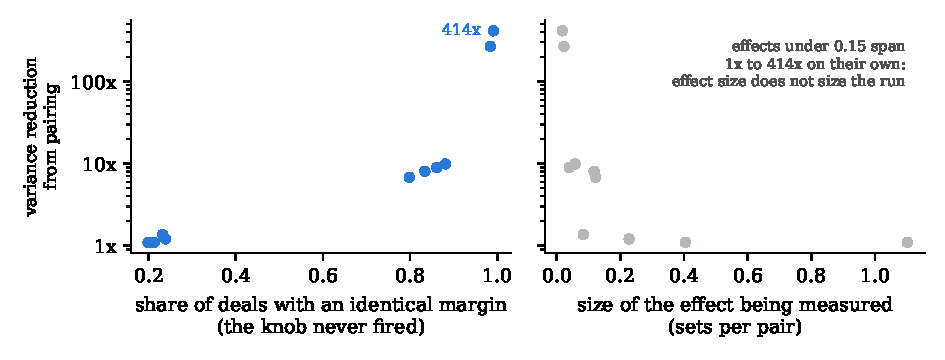
\includegraphics[width=\linewidth]{figs/pairing.pdf}
\caption{What actually sizes a duplicate-deal run. \emph{Left:} the
variance-reduction factor from pairing against the share of deals on which both
arms produced an identical margin --- that is, on which the knob under test
never changed a decision. The relationship is tight over more than two orders
of magnitude. \emph{Right:} the same factor against the size of the effect
being measured, which is the quantity everyone reaches for when planning a run
and which does not determine the answer: effects below $0.15$ sets per pair
span the entire range on their own. Same runs as Table~\ref{tab:pairing}.}
\label{fig:pairing}
\end{figure}

\begin{table}[t]
\centering
\begin{tabular}{llrrr}
\toprule
run & arm & identical games & $\rho$ & efficiency \\
\midrule
$\gamma$ policy specificity (G1) & \texttt{B\_none} & $19.9\%$ & $0.089$ & $1.1\times$ \\
$\gamma$ policy specificity (G1) & \texttt{C\_measured} & $21.2\%$ & $0.088$ & $1.1\times$ \\
signalling gate & \texttt{C\_measured} & $79.8\%$ & $0.853$ & $6.8\times$ \\
signalling gate & \texttt{B\_incumbent} & $83.4\%$ & $0.877$ & $8.1\times$ \\
doomed-ask gate & \texttt{B2\_mid} & $86.1\%$ & $0.889$ & $9.0\times$ \\
doomed-ask gate & \texttt{B\_defer} & $88.1\%$ & $0.899$ & $9.9\times$ \\
forced search, self-play & \texttt{B\_full} & $98.4\%$ & $0.996$ & $268\times$ \\
forced search, vs v0.7 & \texttt{B\_full} & $99.1\%$ & $0.998$ & $414\times$ \\
\bottomrule
\end{tabular}
\caption{How many times the games an unpaired design would need to match the
precision each paired run achieved. ``Identical games'' is the share of games
the two arms finished on the same margin, and it orders the table: a knob that
fires on a rare branch leaves nearly every game bit-identical and pairing
removes almost all the variance, while $\gamma$ re-weights every posterior
sample on every decision, the games diverge immediately, and pairing removes
nothing.}
\label{tab:pairing}
\end{table}

The planning consequence is worth stating plainly, because this project has
sized runs by effect size alone and that is the wrong variable. \textbf{The
sample size a screen needs is governed by how often its knob changes a
decision, not by how large the effect is.} The forced-search secondary
resolved a $+0.0180$ effect to $\pm 0.012$ on $1{,}000$ games; G1, at $1{,}600$
games and the same design, could resolve nothing finer than $\pm 0.19$. That is
a sixteen-fold difference in precision from the same number of deals, and it
is entirely attributable to one knob firing on $0.9\%$ of games and the other
on $80\%$.

\subsection{How much can an experiment of size \texorpdfstring{$n$}{n} resolve?}

The per-pair standard deviation of the set differential between two policies of
the strength we compare (v0.3's champion against its own baseline) is
\textbf{3.869 sets}, measured over 300 pairs. The distribution is wide: the
theoretical bound is $\pm 18$ and observed pairs stayed within $\pm 11$, but a
single pair says almost nothing. The consequences are stark:

\begin{center}
\small
\begin{tabular}{lrrr}
\toprule
effect (sets/pair) & pairs @ 80\% power & pairs @ 90\% & hours @ 80\% \\
\midrule
0.10 & 11\,751 & 15\,731 & 3.9 \\
0.20 & 2\,938 & 3\,933 & 0.98 \\
0.30 & 1\,306 & 1\,748 & 0.44 \\
0.50 & 471 & 630 & 0.16 \\
1.00 & 118 & 158 & 0.04 \\
\bottomrule
\end{tabular}
\end{center}

Read the other way: the 600-pair cells of the v0.3 champion search could resolve
effects down to about $0.44$ sets per pair, so every ``no significant
difference'' it reported below that size was \emph{uninformative rather than
negative}. We therefore report, alongside every interval, the smallest effect
the run could have detected.

\paragraph{That standard deviation is not a property of the game.} The table
above, and every power calculation in this paper up to this point, treats
$3.8$ sets per pair as a constant of the deal population. It is not. It is a
property of a \emph{pair of policies} that disagree constantly, and the
experiments most in need of careful sizing are the ones whose arms barely
disagree at all. We noticed this only when a screening cell measured a per-pair
standard deviation of $2.328$ --- seven standard errors from the figure it had
been sized against.

The mechanism is immediate once stated. Under common random numbers, a deal-pair
on which the two arms play \emph{identically} contributes a difference of
exactly zero. Writing $s$ for the share of pairs on which they diverge at all,
\[
  \operatorname{Var}(D) \;\approx\; s \cdot \operatorname{Var}(D \mid \text{diverge}),
  \qquad\text{so}\qquad
  \mathrm{sd} \;\approx\; \sqrt{s}\;\cdot\;\mathrm{sd}(D \mid \text{diverge}).
\]
That much is arithmetic and follows from the design. The empirical content is
what the second factor does. Across the $46$ cells of this study that store
their per-pair differentials it moves little in absolute terms --- $3.86 \pm
0.29$, a relative spread of $7.6\%$ against $15.5\%$ for the raw standard
deviation --- and our first draft stopped there and called that the finding. It
does not survive being looked at properly.

Three things weaken it, and the third matters for use. \emph{Most of the
residual spread is not structure}: the sampling noise of an $\mathrm{sd}$
estimate at these sample sizes is alone $2.8\%$. \emph{The comparison is carried
by a handful of cells}: restricted to the $26$ cells with divergence share above
$0.83$ --- where most of this study lives --- the raw spread is $3.38\%$ and the
conditional spread is $3.45\%$, the same number to within noise, and the
correlation between share and $\mathrm{sd}$ collapses from $+0.95$ to $-0.03$.
Where share barely varies the decomposition has nothing to explain, and it
explains nothing. And \emph{the conditional term is not constant}: it drifts
with share, $\mathrm{corr} = +0.79$, fitted as $2.53 + 1.66\,s$.

That drift matters precisely where the rule gets used, because the rule is only
useful when extrapolated to a low-divergence contrast. At $s = 0.31$ the flat
model predicts $\mathrm{sd} = 2.18$ and the fitted line predicts $1.68$ --- a
$30\%$ over-estimate. The direction is the saving grace: over-predicting noise
asks for more pairs than are needed, never fewer, so a run sized this way is
over-powered rather than under-powered. But a rule invoked to justify a
\emph{smaller} experiment than the A/A figure implies should not be quoted as
though it were calibrated at the point where it is used, and it is not.

One further caveat on what $s$ means. It is measured as $\Prob(D \neq 0)$, and
$D$ is zero on many pairs where the two arms genuinely diverged and the deal
still ended level --- zero is not an isolated atom in these histograms. So the
cheap substitute the rule advertises, counting disagreements at the level of
decisions rather than of finished pairs, is a strictly larger quantity than the
one the constant was calibrated against, and using it directly would inflate the
predicted noise further.

What survives is narrower than we first wrote and still worth having: the
per-pair standard deviation is a property of the comparison rather than of the
game, the $\sqrt{s}$ scaling is exact by construction, and sizing every
experiment against a figure measured between two maximally-different policies is
systematically conservative for the near-identical comparisons that most need
care.

\label{sec:eval-sd}
\paragraph{The extrapolation was untestable, and then it was tested.} When the
above was written this study had no cells below $s = 0.44$, so the calibration
of the constant at low share --- the only place the rule is ever \emph{used} ---
was not established, and the paragraph said so. The gated re-take run has since
landed two blocks at $s = 0.233$ and $s = 0.236$, and the prediction that the
flat model over-states low-share noise by roughly $30\%$ was recorded in
\path{jobs/PREREGISTRATION_retake_gate.md} \emph{before any pair of that run
was played}. Scoring it out of sample, over the three cells now below $s = 0.5$:
\begin{center}
\begin{tabular}{lrrrr}
\toprule
cell & $s$ & measured sd & flat & drift-corrected \\
\midrule
re-take gate, block 0 & $0.233$ & $1.443$ & $1.863$ & $1.409$ \\
re-take gate, block 1 & $0.236$ & $1.440$ & $1.875$ & $1.420$ \\
ungated re-take penalty & $0.440$ & $2.328$ & $2.560$ & $2.163$ \\
\midrule
\multicolumn{2}{l}{\textbf{mean relative error}} & &
  $\mathbf{+23.1\%}$ & $\mathbf{-3.6\%}$ \\
\bottomrule
\end{tabular}
\end{center}
The flat constant over-predicts by $23\%$ where it is used; the drift-corrected
line lands within $4\%$. This is the only out-of-sample prediction in the paper
that was written down before the data existed and then checked against it, and
it is worth more than the several in-sample fits around it. Sizing at low $s$
should use $\mathrm{sd} = (2.53 + 1.66\,s)\sqrt{s}$, and the flat form remains
the conservative choice --- it asks for more pairs than are needed, never
fewer.

The correlation between $s$ and the raw standard deviation is $+0.952$, and we
report it only to say that it is \emph{not} evidence. If $\mathrm{sd}$ really is
$c\sqrt{s}$ for roughly constant $c$, that correlation is the correlation of $s$
with $\sqrt{s}$, which is near $1$ over any range --- it is implied by the
identity rather than a test of it. A reader will compute it anyway, so it is
better stated and defused than omitted.

Sizing therefore reduces to predicting one quantity, $s$, which can be counted
from \emph{decisions} rather than from finished pairs and is correspondingly
cheap. The consequence is not cosmetic. A candidate that perturbs $10\%$ of pairs
has $\mathrm{sd} \approx 1.23$, not $3.80$: sized on the constant it would need
$9.5\times$ the pairs, which is the difference between an experiment that looks
impossible and one that is routine. We used exactly this to decline a run --- a
sixth cell in a family of five failures, whose largest possible effect we could
show in advance was inside what the cell would resolve, so that it would have
returned a null whatever the truth was --- and to size its honest replacement at
$2000$ pairs rather than the $6200$ the constant demanded.

The direction of the error is worth naming: sizing on the A/A figure is
\emph{conservative}, so nothing already published here is too narrow. What it
cost was experiments never run, and nulls recorded from cells that could not
have found anything. Those are the expensive kind of mistake precisely because
they leave no trace in any interval.

\subsection{Anytime-valid stopping}

Screening many candidate terms invites peeking. A fixed-$n$ 95\% $t$-interval,
monitored after every deal, rejects a \emph{true null} 68.8\% of the time on an
empirical null and 92.1\% on a skewed one, with a median false stop after 11 and
3 deals respectively. We therefore use anytime-valid procedures: an
empirical-Bernstein confidence sequence and a betting test supermartingale
\citep{waudbysmith2024estimating}. Measured type-I error under continuous
monitoring over $4000$ null experiments each monitored at every one of $4000$
deals: 2.1--2.4\% for the betting test and 0.3--0.5\% for the confidence
sequence, against a nominal 5\%.

\subsection{Two corrections to the previous harness}

\paragraph{Timed-out games must be scored, not dropped.} Nothing in Literature
forces progress, so a harness needs an action cap. v0.3 dropped any deal-pair
containing a capped game. Dropping conditions on the outcome, which is precisely
what a paired design exists to avoid, and an audit conducted for this paper
found it biases rather than merely blunts: replaying the same 60 deals at
reduced caps, the dropped pairs had a true mean differential of $-7.14$ against
$-10.13$ for the kept ones, and at one cap the reported 95\% interval
\emph{excluded} the true value. v0.4 scores a capped game on the half-suits
actually resolved, with the unresolved ones counting for nobody --- the same
semantics the exact solver gives an unbroken cycle.

\paragraph{An ablation must reduce to its baseline.} v0.3's most instructive
methodological failure was a confounded ablation: the ablated agent silently
normalised a second term differently, so every cell compared two changes at once
and produced tight, confident, and completely wrong intervals. The confound was
caught only by noticing an implausible monotonic pattern in the magnitudes. We
therefore enforce by test that a zero weight reproduces the baseline
\emph{decision for decision} over real positions, and separately that a non-zero
weight demonstrably changes some decision. Every term in
Table~\ref{tab:terms} passes both.

% =====================================================================
\section{Results: what the inference is worth}
\label{sec:results}

Figure~\ref{fig:effects} is this section on one axis: every in-play effect the
paper settles, each measured by the paired duplicate-deal design of
\S\ref{sec:eval}, sorted by size. The subsections that follow take the rows in
turn; the orange row is measured in \S\ref{sec:critic}.

\begin{figure}[t]
\centering
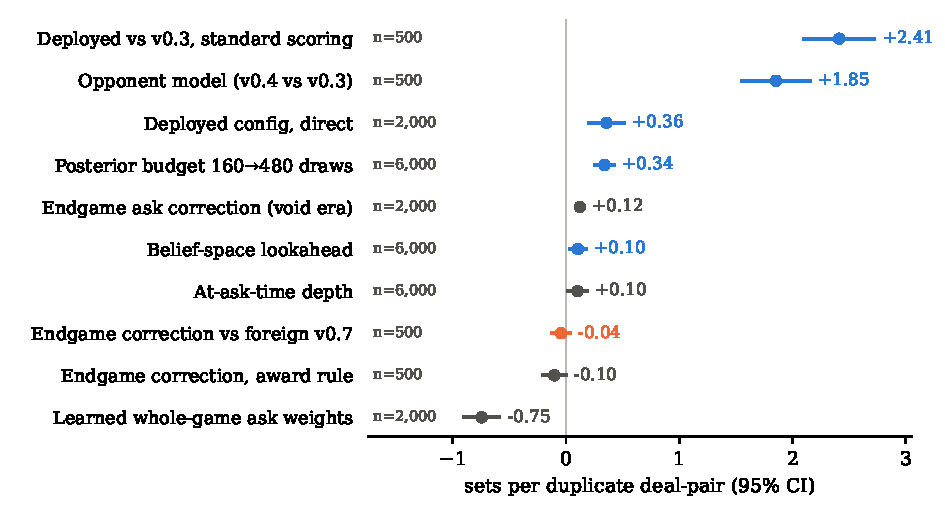
\includegraphics[width=\linewidth]{figs/effects.pdf}
\caption{Every settled in-play effect, on one axis. Blue rows ship in the
deployed configuration; gray rows were evaluated and not shipped ---
at-ask-time depth a null at $n = 6000$, the learned whole-game weights
significantly worse, and the endgame ask correction shipped in the void era
and \emph{withdrawn} when the award baseline re-priced it below zero
(\S\ref{sec:critic}). The orange row is that correction against a foreign
engine, Dylan's FishBot v0.7, under the matched award rule: a tie whose
interval excludes the sibling-measured void-era $+0.12$ --- the paper's
recurring finding that gains measured inside an engine family shrink outside
it. Intervals are 95\% confidence intervals over paired deals; $n$ counts
pairs.}
\label{fig:effects}
\end{figure}

\subsection{Exact inference alone changes nothing}
\label{sec:res-exact}

The first experiment is the one the research programme predicted would pay.
Holding the ask objective at v0.3's champion weights and changing \emph{only}
the inference --- exact counting where the clause set is empty, unbiased
importance sampling where it is not, in place of a sampler documented as
non-uniform --- gives a set differential of $-0.22$ per deal-pair,
95\% CI $[-0.96, +0.52]$, over 100 duplicate deals. Statistically
indistinguishable, and the interval is wide enough that only effects above
about $1.1$ sets per pair could have been detected.

This is a genuine negative result about a change that is provably correct. The
explanation is in the next subsection.

\subsection{Posterior quality against ground truth}
\label{sec:res-posterior}

Scoring posteriors against the true hidden hands over 517 decisions and 13{,}640
uncertain-card predictions (Table~\ref{tab:posterior}) shows what happened.

\begin{table}[t]
\centering
\small
\begin{tabular}{lrrrr}
\toprule
inference & NLL $\downarrow$ & Brier $\downarrow$ & top-1 $\uparrow$ & ms/decision \\
\midrule
exact DP, clauses ignored          & 1.4776 & 0.7568 & 0.287 & 50.4 \\
v0.3 sampler, 32 draws             & 1.4399 & 0.7065 & 0.386 & 5.9 \\
v0.4 importance sampler, 160       & 1.3731 & 0.7006 & 0.396 & 29.5 \\
v0.4 importance sampler, 512       & 1.3618 & 0.6955 & 0.403 & 92.3 \\
v0.3 sampler, 96 draws             & 1.3552 & 0.6891 & 0.406 & 16.6 \\
\textbf{v0.3 sampler, 512 draws}   & \textbf{1.3408} & 0.6833 & 0.416 & 87.8 \\
v0.4 + opponent model, 160, $\gamma{=}0.45$ & 1.3476 & 0.6856 & 0.401 & 31.9 \\
v0.4 + opponent model, 512, $\gamma{=}0.30$ & 1.3332 & 0.6791 & 0.415 & 99.8 \\
\textbf{v0.4 + opponent model, 512, $\gamma{=}0.45$} & \textbf{1.3251} & \textbf{0.6747} & 0.413 & 98.6 \\
v0.4 + opponent model, 512, $\gamma{=}0.60$ & 1.3248 & 0.6744 & 0.411 & 100.8 \\
\bottomrule
\end{tabular}
\caption{How much probability each inference configuration places on where the
cards actually are. Lower NLL and Brier are better. The row that matters is the
comparison between the two bold entries: the \emph{exactly correct} uniform
posterior at 512 draws (1.3618) is worse than v0.3's \emph{biased} sampler at
the same budget (1.3408).}
\label{tab:posterior}
\end{table}

Two things stand out.

First, the exactly-uniform posterior is \emph{worse} at predicting reality than
the heuristic sampler it replaced: $1.3618$ against $1.3408$ at a matched draw
budget. That is not a contradiction. Proposition~\ref{prop:uniform} is a correct
theorem about a false hypothesis. v0.3's sampler seeded the OR-clauses by
picking a live card of the asked half-suit for the asker, which systematically
over-weights worlds in which askers are deep in the suits they asked in --- an
accidental opponent model. Removing the bias removed the model with it.

Second, making the model explicit and tunable recovers the loss and passes both:
$1.3251$ at $\gamma = 0.45$. And the improvement is not a large-budget artefact.
At 160 draws the opponent model takes the sampler from $1.3731$ to $1.3476$,
which is better than v0.3's deployed 32-draw configuration ($1.4399$) by a wide
margin.

Third, and separately: ignoring the OR-clauses is by far the worst option
tested, confirming the design decision of Section~\ref{sec:clauses} from the
other direction.

\subsection{How much of the sampling budget survives reweighting}
\label{sec:res-ess}

Table~\ref{tab:posterior} scores the posterior. This asks what it costs to get
there, and finds a diagnostic that has been computed on every decision this
engine has ever made and reported on none of them.

The posterior is drawn by importance sampling and self-normalised.
Self-normalisation is consistent, not free: if the proposal is a poor match for
the target, a few draws carry most of the weight and the batch behaves like far
fewer than $n$ independent worlds. Kish's effective sample size measures that,
and the sampler already computes it.

At the champion configuration, 160 draws are worth $83.7$ effective --- $52\%$
efficiency --- with a p10 of $64.8$, a median of $87.0$ and a p90 of $100.0$
over $641$ decisions across $36$ seat-deals. The exact DP is almost never the
path taken: $9$ decisions in $641$. So the precision of every
$\Prob(\text{success})$ in this engine is the precision of that one sampled
batch.

\paragraph{A control this paragraph used to claim, and did not have.} Earlier
drafts read ``$83.7$ effective \dots\ against $99.9$ with the opponent model
disabled'', and reported $14$ exact decisions in $646$ for that arm. No such arm
was ever run. \path{results/ess_probe.json} holds four rows, all at
$\gamma = 0.35$, differing only in the proposal tilt; the $99.9$ is the
\emph{p90 of the champion row itself} ($99.986$), and the $14$ in $646$ has no
source at all. A percentile of one arm had been written up as the mean of
another, and the paragraph that followed then explained a gap between them.

That is worth more than a correction, because the argument it supported was
sound and the number under it was not. The efficiency loss from steering the
proposal is real and is measured --- $52\%$ --- and the remedy discussed below
was tested and did make the marginals worse. What was never measured is how
much of the loss the opponent model accounts for, and with $\gamma > 0$ changing
the target the exact DP is built to count, the comparison is not a
straightforward one to run. It is left open rather than asserted.

The gap has an obvious explanation and an obvious remedy, and the remedy is a
trap. The proposal is quota-proportional and knows nothing about the choice
model, so the whole tilt of the target lands in the weights; folding one step of
the likelihood into the proposal is textbook, and it does exactly what the
textbook says --- effective sample size rises to $105.8$, past even the untilted
$\gamma = 0$ figure. Partial strengths are worse than either end, the signature
of a proposal distorted but not matched.

Measured against a high-precision reference, the twist makes the marginals
$3.4\times$ worse.

Effective sample size measures how \emph{flat} the weights are, and a proposal
that covers one corner of the target well and the rest not at all has beautifully
flat weights over the corner it covers. The one-step twist overshoots because the
likelihood's depth-zero term is a numerical floor of $\log 10^{-9}$: the
astronomical $0 \to 1$ ratio makes the proposal read ``this slot is empty now''
as ``this slot ends empty'' and drives nearly every draw into one configuration.
The parameter ships at zero, verified bit-identical to the untwisted sampler, and
the tests pin both halves of the result so that the next person to notice the
efficiency gap does not have to rediscover why closing it fails.

\paragraph{Is precision still worth buying?} v0.3 found belief precision
unsaturated, but with a biased sampler and a different estimator, so it does not
transfer. Measured here against a 16{,}000-draw reference, L1 error per card falls
as $n^{-0.475}$ from 40 draws to 1280 with no bias floor anywhere:

\begin{center}
\small
\begin{tabular}{lrrrrrr}
\toprule
draws & 40 & 80 & 160 & 320 & 640 & 1280 \\
\midrule
L1 per card & 0.248 & 0.174 & 0.128 & 0.091 & 0.066 & 0.048 \\
\bottomrule
\end{tabular}
\end{center}

Two things follow. The exponent is the pure Monte Carlo law, which independently
confirms the sampler is unbiased --- a bias floor would show as the curve
flattening, and it does not. And precision at the operating point of 160 draws is
nowhere near saturated: the prize is real and can be bought directly with draws
rather than with a cleverer proposal.

\paragraph{The policy can feel it, and it is the largest single change here apart from the opponent model.}
\label{sec:res-precision}
The duel that paragraph declined to claim was pre-registered before its
screening cell finished --- deliberately, because the belief-space search had
already cost four rounds partly by being sized against a number a screen had
inflated, and the only reliable defence is to fix the design before the number
exists. It was sized against a \emph{minimum interesting effect} of $+0.15$ sets
per deal-pair rather than against any estimate, on the ground that an effect
smaller than the already-shipped search delivers, for triple the sampling
budget, is not one this engine should adopt.

Six blocks of $1000$ duplicate deal-pairs, $\texttt{n\_draws} = 480$ against
$160$, everything else identical:
\[
  +0.340 \text{ sets per deal-pair}, \quad 95\%\ [+0.243,\, +0.436].
\]
All six blocks are positive, Cochran's $Q = 2.92$ on $5$ degrees of freedom
($p = 0.71$), $I^2 = 0\%$, $\hat\tau = 0$. The entire interval clears the
threshold fixed in advance. For scale, this is more than three times the
belief-space search, which took four rounds and $6000$ pre-registered pairs to
establish at $+0.104$.

The $400$-pair screen of this same cell had read $+0.160$. The confirmatory run
reads $+0.340$ --- \emph{higher}. That is what an unselected screen looks like,
and it is worth stating only because every screen this project \emph{selected}
on inflated instead.

\paragraph{What it costs, and why that is a separate decision.} The
pre-registration committed in advance that a demonstrated effect would not
automatically move the default, because $\texttt{n\_draws}$ trades strength
against latency and the public table has a request budget. Measured on $90$
positions, a decision costs
\[
  3.57\,\mathrm{ms} \;+\; 6.34\,\mu\mathrm{s} \text{ per draw},
\]
a fit whose residuals reach $0.21$\,ms across $40$ to $1920$ draws, and are
worst at the low end --- $-0.21$ at $40$ draws and $+0.20$ at $160$, against
$+0.03$ and $-0.02$ at $480$ and $1920$. So the straight line is a good
description of the expensive end and a rough one exactly where the shipped
budget sits, which is worth knowing before using it to price a change at $160$.
The ratio quoted next does not depend on it: it is measured per decision, not
read off the fit. At the
shipped $160$ the sampler is only a fifth of a decision, so tripling it costs
$+1.9$\,ms --- $1.38\times$, not $3\times$. That headroom is finite and the same
fit says so: by $1920$ draws a decision is already $3.3\times$ the shipped one.
With the effect and the price both measured, the default moved to $480$.

That fit is not an explanation, and the difference matters: if the fixed term
were setup, it could be hoisted and draws would become nearly free. Timing the
sampler alone, on one already-built sampler across $1$ to $1440$ draws, gives
$2.50\,\mathrm{ms} + 8.0\,\mu\mathrm{s}$ per draw --- about $60\,\mu$s of fixed
cost for each of the $42$ free cards it must place. That is per-card numpy
dispatch. Sequential importance sampling walks the free cards one at a time, so
batching makes each \emph{step} wider without making the number of steps
smaller, and the per-card constants are already cached. There is nothing there to
hoist.

The consequence is a design rule with a number attached: going from $160$ to
$480$ draws costs $2.2$\,ms inside the sampler, while going from one decision to
two costs $2.5$\,ms before a single draw is taken. Draws are cheap and decisions
are expensive, so under a latency budget a better posterior at one decision beats
more decisions with worse ones. The belief-space search of
Section~\ref{sec:lookahead} already obeys this without having been designed to: it
never samples, and operates on the single posterior marginal matrix it is handed.

One caution on those two fits. The per-draw slope of the sampler alone
($8.0\,\mu$s) exceeds that of the whole decision containing it ($6.34\,\mu$s),
which is impossible until the position mix is accounted for: per-draw work scales
with the number of free cards, and the two runs drew positions averaging $42$ and
$28$ of them. Scaling by that ratio predicts $5.4\,\mu$s against the $6.34$
measured, which restores the ordering and accounts for most of the gap but not
all of it --- the remainder is the rest of a decision that also grows with the
draw count. We report it as a partial reconciliation rather than a clean one.

Two of this paper's four documented winner's curses were paid for by sizing an
experiment against an inflated screen. This is the case where pre-registering
against a threshold instead cost nothing and returned the study's largest
result.

\subsection{The opponent model in play}
\label{sec:res-oppmodel}

Posterior accuracy is not strength. Table~\ref{tab:gamma} measures the model by
duplicate-deal play against the otherwise-identical $\gamma = 0$ policy.

\begin{table}[t]
\centering
\small
\begin{tabular}{lrrl}
\toprule
$\gamma$ & pair score & set diff / pair & 95\% CI \\
\midrule
0.10 & 0.613 & $+0.993$ & $[+0.470, +1.517]$ \\
0.30 & 0.667 & $+1.847$ & $[+1.230, +2.463]$ \\
0.45 & 0.700 & $+1.860$ & $[+1.336, +2.384]$ \\
0.60 & 0.657 & $+1.300$ & $[+0.795, +1.805]$ \\
0.90 & 0.723 & $+1.827$ & $[+1.199, +2.455]$ \\
\bottomrule
\end{tabular}
\caption{Opponent model against the identical policy with the model disabled,
150 duplicate deal-pairs per cell. Every cell excludes zero. The dose-response
rises to a plateau by $\gamma = 0.30$ and stays there over a threefold range,
which is what one wants from a model with a single free parameter --- and unlike
the ask-objective terms of v0.3, which showed a sharp inverted-U, there is no
weight at which this becomes destructive within the range tested.}
\label{tab:gamma}
\end{table}

\paragraph{The cleanest attribution.} Tables~\ref{tab:gamma} measures the model
against copies of itself. The sharper experiment holds the \emph{opponent} fixed
at the v0.3 champion and varies only whether the model is on, at identical deal
seeds and identical agent seeds, 250 duplicate deal-pairs each:

\begin{center}
\small
\begin{tabular}{lrrl}
\toprule
v0.4 configuration & pair score & set diff / pair & 95\% CI \\
\midrule
exact inference, $\gamma = 0$ & 0.502 & $-0.008$ & $[-0.482, +0.466]$ \\
exact inference, $\gamma = 0.30$ & 0.684 & $\mathbf{+1.920}$ & $[+1.479, +2.361]$ \\
\bottomrule
\end{tabular}
\end{center}

The first row is as close to exactly zero as a 250-pair experiment can report.
Provably correct inference, replacing a sampler its own authors documented as
biased, moved the result by eight thousandths of a set per deal-pair. The second
row differs from the first in one parameter.

\subsection{The choice model, measured rather than assumed}
\label{sec:res-choicecurve}

Section~\ref{sec:res-oppmodel} establishes that the model is worth $+1.9$ sets
per deal-pair, which is the largest single effect in this engine. It rests on
one sentence: \emph{a player asks in a half-suit in proportion to how many cards
of it they hold}. Proportional means an exponent of one, and that exponent was
never measured. It was chosen because it is the one value whose denominator is
public --- the depths of a hand sum to its size --- which is an excellent reason
to try it and no reason whatever to believe it.

There is a specific reason to doubt it. Under an objective dominated by
$\Prob(\text{success})$, what makes a half-suit worth asking in is how many cards
it still offers: holding five of six offers exactly one card to ask for, holding
one of six offers five. Depth and opportunity pull in opposite directions, so
linear-in-depth is not obviously right even in sign.

\paragraph{The design.} The policy is available, so the propensity can be
measured instead of argued. Over 200 self-play games we record, at every ask,
which half-suits were legal, the asker's depth in each \emph{on the initial
deal}, and which was chosen. That is a conditional-logit design in which the
alternatives are known from the rules rather than inferred, and it yields 17{,}005
asks where at least two half-suits were legal --- 72{,}091 alternatives in all.
Fitting $\Prob(\text{ask in }H) \propto \operatorname{depth}_H^{\alpha}$ by exact
conditional likelihood gives $\alpha$ directly, with $\alpha = 1$ the shipped
model and $\alpha = 0$ legality carrying all the signal and depth none.

Standard errors are block-bootstrapped over games. This is not a refinement: the
likelihood's own curvature treats every decision as an independent draw, and
17{,}005 decisions come from 200 deals whose members share a layout, six hands and
one set of policies. The correction doubles every interval, and the symptom was
visible beforehand --- a smooth curve through the per-band estimates returned a
$\chi^2$ several times its degrees of freedom.

\begin{table}[t]
\centering
\small
\begin{tabular}{lrrrrrrr}
\toprule
half-suits resolved & 0 & 1 & 2 & 3 & 4 & 5 & 6--8 \\
\midrule
$\alpha$          & $2.00$ & $1.28$ & $1.20$ & $0.68$ & $0.30$ & $0.41$ & $-0.02$ \\
clustered SE      & $0.08$ & $0.08$ & $0.12$ & $0.12$ & $0.13$ & $0.18$ & $0.16$ \\
decisions         & 4410 & 2881 & 2527 & 2437 & 1958 & 1541 & 1251 \\
\bottomrule
\end{tabular}
\caption{The fitted exponent of the choice model against how far the deal has
run. The shipped model is a constant $1$. It is wrong at both ends, in opposite
directions: at the opening the true exponent is about $2$ and the model
understates its own strongest signal, and by the endgame it is $0$ and the model
applies a tilt that is not there.}
\label{tab:choicecurve}
\end{table}

\paragraph{What it says.} Pooled over the whole game the best constant is
$\alpha = 1.207 \pm 0.046$ --- close enough to $1$ that a constant never looked
broken, and far enough from either end of Table~\ref{tab:choicecurve} that it
could not be right. Split at the halfway point, $\alpha = 1.331 \pm 0.049$ early
against $0.232 \pm 0.118$ late. The likelihood prefers the fitted constant to
$\alpha = 0$ by 1402 nats and to $\alpha = 1$ by 40.

\paragraph{And most of the decay is the covariate, not the player.} The obvious
reading of Table~\ref{tab:choicecurve} is behavioural: a player asks where they
are deep only if they had a choice, and late, holding two cards with most of the
deck resolved, legality binds. That reading is largely wrong, and the same
17{,}005 decisions say so.

The fit conditions on depth \emph{on the initial deal}, because that is what the
sampler assigns. Cards move, so as a game runs on that covariate drifts from the
hand the asker actually held --- mean absolute disagreement rises from $0.16$
cards at the opening to $0.66$ by the endgame, with correlation falling from
$0.77$ to $0.44$. Noise in a covariate attenuates its coefficient, and noise that
grows with the game manufactures precisely this decay. Refitting on depth at the
moment of the ask:

\begin{center}
\small
\begin{tabular}{lrrrrr}
\toprule
covariate & opening & 1--2 & 3--4 & 5--8 & pooled \\
\midrule
initial-deal depth & $2.00$ & $1.25$ & $0.52$ & $0.23$ & $1.207$ \\
depth at the ask   & $2.90$ & $2.32$ & $1.72$ & $1.34$ & $2.195$ \\
\bottomrule
\end{tabular}
\end{center}

The decay survives and shrinks, and never approaches zero. Late asks do carry
depth signal; what decays is how well the initial deal still describes the hand
it is about.

\paragraph{The better covariate is free.} Depth at the moment of the ask looked
expensive --- it appeared to need the public history replayed against every
candidate world --- and it is not, because of a fact about the rules. Cards move
only when an ask succeeds, and a successful ask is entirely public: the card, the
asker and the target are all in the log. So
$\text{depth}_{\text{at ask}}(p,H) = \text{depth}_{\text{initial}}(p,H) +
\delta(p,H,t)$ with $\delta$ \emph{identical in every hypothesised world}. The
sampler goes on assigning initial deals and the likelihood adds a constant known
before any drawing. Verified against the engine on 23{,}268
(player, half-suit, time) triples across six games, with no mismatches.

Measured as a description, the difference is not marginal: at-ask-time depth
fits the same choices $4{,}654$ nats better, reaching $6{,}057$ nats above
uniform where the initial deal reaches $1{,}403$. The shipped covariate captures
under a quarter of what its own one-parameter family can.

This is not the \texttt{attime} mode of Section~\ref{sec:res-null}, which
computes belief-\emph{located} depth and adds a present-tense count to free cards
drawn over the initial deal; that mode measured $-1.544$ sets per deal-pair over
250 pairs. Whether the exact version plays better is a duel, and is not claimed
here.

\paragraph{Is the power law the right shape?} Fitting one functional form well
is not evidence that it is the right one. The saturated alternative gives every
depth value a free coefficient; it nests the power law, so it can never fit
worse, and it is the best that anything conditioning on depth alone can do. On
the same decisions the power law gives up $110$ nats to it on initial-deal depth
and $269$ on depth at the ask.

Set against the $4{,}654$ nats that changing the covariate is worth, the shape is
not what limits this model --- the covariate matters roughly seventeen times
more. That is the useful bound: further gains in the choice model need a
different conditioning variable or the normaliser below, not a better curve.
(The initial-deal figure is a lower bound; that fit had not converged, and its
depth-5 coefficient rests on five alternatives in the whole corpus.)

\paragraph{What the engine drops, and where it sits.} The likelihood is written
as proportional to a product of depths, and the proportionality hides a
denominator: a proper choice model divides by the sum of $\text{depth}^\alpha$
over the half-suits the player could legally ask in. At $\alpha = 1$ that sum is
the player's hand count --- public, identical in every world, and it cancels.
That is the original argument for an exponent near $1$, and it holds for every
covariate here: the depths over live half-suits sum to the hand count whether
depth is read at the deal, now, or at the ask.

The cost of being elsewhere had never been measured. Across worlds drawn from
the posterior at 30 real positions, the coefficient of variation of the dropped
denominator is

\begin{center}
\small
\begin{tabular}{lrrrrrrr}
\toprule
$\alpha$ & $0.35$ & $0.60$ & $0.80$ & $1.00$ & $1.207$ & $1.60$ & $2.195$ \\
\midrule
mean CV & $0.100$ & $0.063$ & $0.032$ & $\mathbf{0.000}$ & $0.035$ & $0.107$ & $0.226$ \\
\bottomrule
\end{tabular}
\end{center}

a V centred exactly on $1$, with the $\alpha = 1$ column serving as the control
that the measurement is reading the right quantity. Two readings follow. The
shipped $\gamma = 0.35$ pays more for the omission ($0.100$) than the fitted
exponent on its own covariate would ($0.035$ at $1.207$) --- the approximation
that motivated an exponent near $1$ is being violated more at the setting in use
than at the one the data prefer. And $\gamma = 1.0$ is not just another point on
the sweep of Table~\ref{tab:gamma}: it is the unique exponent at which this
likelihood is correctly specified. That sweep never tested it; $0.90$ and $1.50$
bracket it at 150 pairs each, an MDE of $0.87$, which separates nothing.

\paragraph{Every number above was measured on one population, and against a
foreign policy the exponent changes sign.} The corpus behind
Table~\ref{tab:choicecurve} is this engine playing a copy of itself. That is
the population the opponent model is used in \emph{when the table is all one
engine}, and it is also the one population in which the assumption cannot
fail: a policy that asks where it is deep, modelled by a policy that assumes
opponents ask where they are deep, will confirm itself.

The obvious control had never been run. Repeating the identical design ---
same alternatives, same covariate, same conditional likelihood, same block
bootstrap over deals, with only \emph{whose asks are recorded} changed ---
against v0.7 over $6{,}090$ of its asks in $150$ cross-engine games gives

\begin{center}
\small
\begin{tabular}{lrrrr}
\toprule
depth on the initial deal & $1$ & $2$ & $3$ & $4$ \\
\midrule
observed / expected & $1.258$ & $0.762$ & $0.548$ & $0.656$ \\
\bottomrule
\end{tabular}
\end{center}

\noindent and a fitted $\alpha = \mathbf{-1.0041}$, 95\%
$[-1.1434, -0.8648]$, against this engine's own $+1.2071$ on the same
estimator. The signs are opposite and the exponents lie $2.21$ apart. A
sampler applying $\gamma = +0.35$ to that seat is not merely mis-scaled; it
re-weights the world set in the wrong direction on every one of that seat's
asks, and every marginal the ask objective and the declaration gate read is
drawn from the result.

The mechanism was written down in this project before it was checked, and then
not checked. Section~\ref{sec:res-choicecurve}'s own premise notes that depth
and opportunity pull opposite ways --- holding five of six leaves one card to
ask for, holding one of six leaves five --- so linear-in-depth was never
obviously right \emph{in sign}. v0.7's objective is dominated by a single
coefficient on $\Prob(\text{success})$ roughly three times its next largest,
which is precisely the objective that prefers the shallower half-suit because
it offers more cards to name. What the self-play corpus measured was not a law
of the game but a fixed point of one policy against itself.

Two conclusions, and the second is the load-bearing one. The narrow one is
that the limit on this model is not the curve's shape (worth $110$ nats) or
even the covariate (worth $4{,}654$): it is that a single global exponent
cannot describe a mixed table, and both of those bounds were computed inside
the population where the exponent happens to be constant. The broad one is a
warning this paper is in a position to give and few others are: \emph{an
opponent model validated only in self-play has been validated against the
assumption it encodes}. Nothing in the fit diagnostics of
\S\ref{sec:res-choicecurve} --- not the $1402$-nat margin over $\alpha = 0$,
not the saturated-alternative comparison, not the phase split --- could have
detected this, because all of them are computed on the same self-consistent
corpus. It took a second engine.

We are deliberately not shipping a per-seat exponent on the strength of this.
The measurement identifies where our inference is wrong about \emph{one}
opponent, and \S\ref{sec:critic} records what happened the last time this
project turned an opponent-model discrepancy into a knob: the gains grew with
the dose and evaporated against a third engine, because what was being
measured was deception of a sibling's inference rather than strength. A
per-seat exponent fitted on v0.7 and validated on v0.7 would reproduce that
error exactly. It needs its own pre-registration and a foreign opponent that
is not the one it was fitted on.

\paragraph{It got one, and the answer is that describing his asks well and
beating him are different problems.} The pre-registration is
\texttt{prereg/gamma\_policy\_specific.md}, written before a game was played,
and it fixed two things in advance: that nothing would ship on a run whose
treatment arm was both fitted on v0.7 and measured against v0.7, and that the
smallest effect worth adopting was $+0.15$. Three arms, identical in every
respect but one scalar, played on $1{,}600$ games ($800$ deals in both seat
parities), each arm seeing the identical deal from the identical seat:

\begin{center}
\small
\begin{tabular}{llrr}
\toprule
arm & $\gamma$ & sets/game & paired difference vs shipped \\
\midrule
A, shipped        & $+0.35$ & $+2.3613$ & --- \\
B, no model       & $\phantom{+}0.00$ & $+1.9563$ & $-0.4050$ $[-0.5911, -0.2189]$ \\
C, his exponent   & $-1.00$ & $+1.2588$ & $-1.1025$ $[-1.2897, -0.9153]$ \\
\bottomrule
\end{tabular}
\end{center}

\noindent Both directions lose, and the fitted one loses by more than twice as
much as switching the model off. The exponent that maximises the likelihood of
v0.7's asks is, in play against v0.7, worse than an exponent with the wrong
sign and worse than no opponent model at all.

That is not a paradox once the two objects are named apart. The fit is a
\emph{marginal} description of which half-suit a policy names, estimated on
depth in the initial deal. The sampler uses it as a \emph{conditional}
likelihood, applied to a world set that has already been cut down by the
no-bluff certifications, the failed asks and the resolved sets --- and it is
scored not by how well it predicts the next ask but by where it puts posterior
mass over card locations. A re-weighting can be better calibrated about his
choices and worse about his cards. Nothing in the estimator we used, which is
the standard one, has any purchase on that distinction: it was never asked to.

So the honest position is narrower than either the worry or the reassurance.
The self-play validation of \S\ref{sec:res-choicecurve} really was circular,
and finding that out took a second engine. But the repair the circularity
seemed to imply --- adopt the exponent the foreign data want --- is measurably
worse than the error, and the pre-registration is what stops that from being
discovered after the fact. Arm C does not clear $+0.15$; G2, against the v0.3
champion, therefore does not run, and nothing ships.

\paragraph{And in play, it is real and not worth buying.}
\label{sec:res-atask} Everything above is an
argument from likelihood and from a normaliser, not from a duel, so the
configuration it points at --- at-ask-time depth at $\gamma = 1.0$, the better
covariate at the exponent where the model is correctly specified --- was
pre-registered and run. Six blocks of 1000 duplicate deal-pairs against the
champion, sized against a minimum interesting effect of $+0.15$ fixed in
advance, with the run committed to proceed whatever its five screening cells
said. They said $-0.05$, $+0.08$, $+0.32$, $-0.13$ and $+0.01$, every one of
them uninformative at $\pm 0.53$, which is why they were never load-bearing.

\[
  +0.1015, \quad 95\%\ [+0.0063,\, +0.1967].
\]

The interval excludes zero, so by the test fixed in advance the effect is
demonstrated. Three things belong next to that, and all three were decided
before the data:

It is \emph{below the bar it set itself}. The pre-registration named $+0.15$ as
the smallest effect worth adopting --- roughly what the belief-space search
delivers --- and this is $+0.10$, with the interval's upper end barely reaching
it. Real, and not worth buying. The threshold was chosen before the number, so
that judgement is not a reaction to it.

The blocks \emph{disagree}. Cochran's $Q = 12.9$ on 5 dof ($p = 0.024$),
$I^2 = 61.4\%$, $\hat\tau = 0.150$ --- the same size as the pooled effect. Two
explanations fit that on its own: the harness understates its uncertainty, or
this particular effect varies with the deal population. They are distinguishable,
because the identical six-block design has now been run three times and the A/A
null twenty-four times:

\begin{center}
\small
\begin{tabular}{lrrrr}
\toprule
run & pooled & $Q$ & $p$ & $\hat\tau$ \\
\midrule
lookahead settling & $+0.104$ & $4.08$ & $0.538$ & $0.000$ \\
precision, 480 vs 160 & $+0.340$ & $2.92$ & $0.713$ & $0.000$ \\
at-ask depth, $\gamma = 1.0$ & $+0.102$ & $12.94$ & $\mathbf{0.024}$ & $\mathbf{0.150}$ \\
A/A null, 24 blocks & $0.000$ & $18.41$ & $0.735$ & $0.000$ \\
\bottomrule
\end{tabular}
\end{center}

Every other run gives $\hat\tau$ \emph{exactly} zero, including two real effects
of comparable and larger size, and so does the null. So the harness is not
understating its uncertainty by default, and a deal-population-dependent effect
is the better explanation here. We state the multiplicity rather than leave it
implicit: four homogeneity tests at the $5\%$ level give roughly a one-in-five
chance of at least one significant result under a complete null, so one
significant $Q$ out of four points at where to look and does not settle it.

The verdict rests on \emph{two of the six blocks}. Leaving out block 0 gives
$[-0.041, +0.168]$ and leaving out block 4 gives $[-0.060, +0.148]$; dropping
either one alone puts zero back inside. No block may be dropped for its result
and none is --- the pre-registered pool is the pool --- but under $I^2 = 61\%$,
with the interval clearing zero by $6.7\%$ of its own half-width, saying so costs
nothing and omitting it would be a choice.

The random-effects interval is $[-0.052, +0.255]$ and \emph{includes zero}. We
report it and it decides nothing. The fixed-effect pool was fixed as primary
before any of this was known, and adopting a wider estimator once the narrow one
is inconvenient is the failure this whole protocol exists to prevent --- it is
the winner's curse run backwards, choosing the analysis that gives the answer
one now prefers. Both numbers are printed; the pre-registered one governs.

So the normaliser argument survives contact with play, and the engine keeps
$\gamma = 0.35$ and initial-deal depth anyway. The two parameters were argued
for jointly and the screens cannot separate them, so the pre-registration binds
them to move together or not at all; they do not move.

\paragraph{The competing story is refuted by the same data.} If asks went where
the opportunity was rather than where the depth was, propensity would fall as
cards held rises. Observed over expected runs $0.46$, $1.05$, $2.26$, $2.64$,
$2.90$ for one through five cards held --- monotonically the other way. Whatever
else is wrong with the model, its sign is right.

\paragraph{A rule, not a regularity.} In 72{,}091 legal alternatives, not one had
an initial-deal depth of zero. That is a theorem rather than a coincidence:
asking in a half-suit requires holding a card of it, and cards move only to
askers who already hold one, so a player's first card of any half-suit cannot
have arrived by play. The consequence matters for the implementation, because
the likelihood floors a zero depth at $\log 10^{-9}$ and that floor is therefore
excluding worlds the \emph{rules} forbid rather than softening an awkward case.
The engine's \texttt{allow\_bluff\_asks} variant does not undo it; that flag
widens which cards of a half-suit may be asked for and leaves the half-suit
guard alone.

\paragraph{What was changed, and what was not.} \texttt{gamma\_schedule}
interpolates between the constant and a weighted quadratic through
Table~\ref{tab:choicecurve} ($\chi^2 = 8.3$ on 4 dof), clamped flat past its
vertex because past there the parabola turns up and the measurements do not.
Given the paragraph above it is best read as a \emph{dilution correction}: the
engine conditions on initial-deal depth, that covariate degrades as the game
runs on, and a degrading covariate should be believed less. That is a more modest
claim than the behavioural one this was first written up as, and a better
supported one --- and it predicts the term should become unnecessary under the
at-ask-time covariate, where nothing drifts. It
is normalised by the profile's mean over the observed distribution of asks, so
full strength redistributes the model's belief across the game without changing
how much of it there is in total. That separation is deliberate: $\gamma$ was
already tuned by duels to the broad plateau of Table~\ref{tab:gamma}, and a term
that moved shape and strength together would leave any positive result
unattributable. Zero remains the incumbent, decision for decision.

Whether the reshaped model plays better is a duel, and is not claimed here.

\paragraph{Limitation.} This measures the champion against copies of itself,
which is exactly the situation the opponent model is used in throughout this
paper, and exactly not the situation of a human table. The profile is a fact
about this policy's behaviour, not about Fish.

% =====================================================================
\section{Strength, absolute and relative}
\label{sec:strength}

\subsection{The strength ladder}
\label{sec:res-ladder}

\begin{table}[t]
\centering
\small
\begin{tabular}{lrrll}
\toprule
v0.4 champion versus & pairs & pair score & set diff / pair & 95\% CI \\
\midrule
\textbf{v0.3 champion (\texttt{tuned})} & \textbf{500} & \textbf{0.705} & $\mathbf{+1.854}$ & $\mathbf{[+1.542, +2.166]}$ \\
\quad --- replication & 300 & 0.758 & $+2.440$ & $[+2.052, +2.828]$ \\
\quad --- replication, $\gamma = 0.30$ & 250 & 0.684 & $+1.920$ & $[+1.479, +2.361]$ \\
v0.3 \texttt{probabilistic}    & 200 & 0.792 & $+2.785$ & $[+2.274, +3.296]$ \\
\bottomrule
\end{tabular}
\caption{The v0.4 champion is
\texttt{fishbot4($\gamma$=0.35)}: exact/unbiased inference, the opponent choice
model, and v0.3's own ask weights. No new objective term is enabled. Every
row was played under the void-era misdeclaration rule; the standard-scoring
restatement of this ladder's headline --- the full deployed configuration
against the v0.3 champion, both sides pricing misdeclarations correctly ---
is $+2.412$ $[+2.088, +2.736]$ over $500$ fresh pairs
(design R1 of \texttt{prereg/rules\_award\_baseline.md},
\texttt{results/award\_headline.json}; wholly-held half-suits declared with
the wrong split, and so awarded to the opponents: $125$ against the deployed
side, $146$ against v0.3. That counter is the allocation class alone --- a
declaration naming a card the opponents actually held is a gift rather than a
misdeclaration and is counted separately, \texttt{fish4/match.py}).}
\label{tab:ladder}
\end{table}

Against the two weakest rungs the champion wins every pair: $120/120$ against
the public-information heuristic ($+14.09$ sets per pair) and $80/80$ against
random ($+16.30$). Those are reported for completeness rather than as evidence;
a shutout means the rating gap is a bound, not a measurement.

The headline comparison was run three times at different seeds, and the three
estimates span $+1.85$ to $+2.44$ --- wider than their individual intervals
suggest, which is a useful reminder that a 95\% interval covers the mean of the
deals actually played, and that three such intervals will occasionally fail to
overlap. We take the largest experiment as the headline and report the others
rather than the most flattering one.

\paragraph{What the strongest configuration is worth, and what nobody has
played.} Two changes in this version clear a pre-registered bar against the
champion: the tripled posterior sampling budget at $+0.340$ and the
belief-space search at $+0.104$. Each was measured against the champion
\emph{alone}, so neither says what their combination is worth --- and the
combination is not obviously additive, since the search's whole mechanism is to
search a belief the sampler draws.

The stacking run lets the two be chained, because it measured the search
\emph{on top of} $480$ draws. The two runs use disjoint deal seeds, so they are
independent and their standard errors add in quadrature:
\begin{center}
\begin{tabular}{lrr}
\toprule
link & estimate & pairs \\
\midrule
$480$ draws vs.\ champion & $+0.340 \pm 0.049$ & 6000 \\
search on top of $480$ draws & $+0.072 \pm 0.042$ & 6000 \\
\midrule
\textbf{chained: search $+$ $480$ draws vs.\ champion}
  & $\mathbf{+0.411 \pm 0.064}$ & 12000 \\
\bottomrule
\end{tabular}
\end{center}
$95\%$ CI $[+0.285, +0.538]$ --- larger than either change alone and, apart
from the opponent model itself, the largest figure in this paper. It is not the
largest \emph{single} change: that is the sampler's $+0.340$, and this number is
two changes at once.

\paragraph{And it has now been played directly, which is the only reason the
number above can stand unqualified.} A chained estimate inherits both links'
assumptions --- in particular that each change's effect does not depend on the
deal population the other was measured over. That was plausible, since both
pools were drawn the same way, and it was \emph{unmeasured}; this paper's
recurring failure is exactly a plausible unmeasured step carrying a published
number. There was also a cheaper reason to run it: \textbf{nobody had ever
played the shipped configuration against the reference in a single duel}, so
every ``vs.\ champion'' figure in this document was for a spec that is not the
one on the website.

\path{jobs/PREREGISTRATION_combined.md} fixes, before any pair: two blocks
of $1000$ fresh pairs; the A/A $3.796$ as the per-pair standard deviation
rather than the divergence model, deliberately conservative because this arm
differs from the champion by \emph{two} knobs and the model was fitted on arms
differing by one; a fixed-effect pool as the only thing that decides; and three
outcomes named in advance --- agrees, lower, higher --- so none could be chosen
afterwards. It also states, in advance, that at $2000$ pairs against the
chain's $12000$ this run \emph{cannot} make the estimate more precise. Its job
is to make it honest, and a wider interval is the design working rather than a
disappointment.

\begin{center}
\small
\begin{tabular}{lll}
\toprule
& estimate & \\
\midrule
chained, 12000 pairs & $+0.411$ $[+0.285, +0.538]$ & indirect \\
\textbf{direct}, 2000 pairs & $\mathbf{+0.357}$ $[+0.191, +0.524]$ & \textbf{excludes zero} \\
\midrule
difference & $-0.054 \pm 0.107$ & does not resolve \\
\bottomrule
\end{tabular}
\end{center}

\textbf{The chain agrees.} The intervals overlap and the difference is half a
standard error, so the assumption the chain rests on is now measured and holds,
and the indirect caveat can leave this section. Worth noting separately: the
design's sizing assumption held almost exactly --- a planned per-pair standard
deviation of $3.796$ against a realised $3.801$ --- which is unusual enough in
this study to be worth one clause, given that the claim-threshold run's
equivalent came in $21\%$ low.

What is \emph{not} settled by this is whether the combination beats the sampler
\emph{alone}: that is the stacking run's own estimate, whose interval contains
zero at $68\%$ power. So the defensible ordering remains
\[
  \text{search}+\text{sampler} \;\ge\; \text{sampler} \;>\; \text{champion},
\]
with the first inequality undemonstrated --- and the leftmost quantity now
measured directly rather than assembled. The engine names this configuration
\texttt{V04\_COMBINED} and the public table has been playing it all along;
until this run reported, no figure in this paper described what the website was
actually running.

\paragraph{And it stops paying: precision's returns diminish.} If tripling the
sampling budget is worth $+0.340$, the obvious question is whether tripling it
again is worth as much. Pre-registered in
\path{jobs/PREREGISTRATION_precision2.md} with a \emph{minimum interesting
effect} of $0.150$ fixed before any pair was played --- so that a small positive
would be reported as a small positive rather than promoted:
\begin{center}
\begin{tabular}{lrl}
\toprule
rung & set diff & 95\% CI \\
\midrule
$160 \to 480$ draws, 6000 pairs & $\mathbf{+0.340}$ & $[+0.244, +0.436]$ \\
$480 \to 1440$ draws, 6000 pairs & $+0.094$ & $[-0.002, +0.191]$ \\
\midrule
\textbf{difference} & $\mathbf{-0.245 \pm 0.069}$ & $\mathbf{-3.5}$ SE \\
\bottomrule
\end{tabular}
\end{center}
Cochran's $Q = 4.01$ on $5$ df ($p = 0.55$), $I^2 = 0\%$, $\tau = 0$: the six
blocks of rung 2 agree with each other completely, and with zero.

Rung 2 on its own is \textbf{not demonstrated} --- its interval includes zero
and its point estimate sits below the $0.150$ threshold fixed in advance. But
the \emph{contrast} is demonstrated, and it is the more interesting quantity.
Both rungs multiply the budget by exactly three, so under a log-linear response
they would buy the same amount. They do not: the difference between the rungs
is $-0.245 \pm 0.069$, which excludes zero at $3.5$ standard errors.
Precision's returns diminish, and they do so somewhere between $480$ and $1440$
draws.

That is worth putting beside the earlier claim it repairs. The failed-experiment
section reported ``precision has saturated'' on the strength of $200$-pair
screens around $160$ draws, and Section~\ref{sec:res-precision} refutes that:
saturation had not begun at $160$. It has begun by $480$. The screens reached
the right word for the wrong rung, and getting from one to the other took
$12{,}000$ pre-registered pairs across two runs.

The default stays at $480$. Rung 1 is demonstrated and bought; rung 2 is not
demonstrated, costs a further $1.4\times$ on the sampler, and its own
pre-registration says a point estimate below $0.150$ does not move a default
whatever its sign.

\paragraph{A demonstrated effect that is deliberately not shipped.} At-ask-time
depth at $\gamma = 1.0$ measures $+0.102$ over $6000$ pre-registered pairs and
its interval excludes zero, so the effect is real. It is also below the $0.15$
that \path{jobs/PREREGISTRATION_at_ask.md} fixed \emph{in advance} as the
smallest effect worth adopting, and the upper end of its interval, $+0.197$,
barely reaches that. It therefore does not ship, and \texttt{depth\_mode} stays
\texttt{"initial"} in every named configuration. A real effect below a threshold
chosen before the data is not a reason to move a default; deciding otherwise
after seeing $+0.102$ is exactly what fixing the threshold in advance prevents.
A test asserts the default, so the decision cannot quietly reverse itself.

\paragraph{Do v0.3's objective terms survive better inference?} A reasonable
worry about the whole result is that v0.3's hand-tuned tie-breakers were
compensating for a poor posterior and would become redundant once it improved.
They do not become redundant, but they do become \emph{worth less}. Removing
both --- setting $w_{\mathrm{turn}}$ and $w_{\mathrm{scarce}}$ to zero and
changing nothing else --- costs, over 250 duplicate deals each:

\begin{center}
\small
\begin{tabular}{lrl}
\toprule
inference & cost of removing both terms & 95\% CI \\
\midrule
without the opponent model & $1.660$ sets/pair & $[+1.240, +2.080]$ \\
with the opponent model    & $1.084$ sets/pair & $[+0.611, +1.557]$ \\
\bottomrule
\end{tabular}
\end{center}

v0.3 measured the same pair at $+1.41$ against its own inference, which sits
between the two. So the terms and the opponent model are partially substitutable:
about a third of what the tie-breakers were contributing is absorbed once the
posterior knows more about opponents' holdings, and the remaining two-thirds is
positional judgement that no amount of card-reading supplies. That is the
expected shape if the tie-breakers were doing two jobs --- compensating for a
blurry posterior, and encoding something genuinely strategic --- and it is worth
noting that the gains do \emph{not} simply add: $1.85$ (the headline) is less
than $1.92$ (the model alone against the v0.3 champion) plus anything.

\subsection{Absolute strength: agreement with provably optimal play}
\label{sec:res-absolute}

Every number above is relative. Table~\ref{tab:exact} is not. It reports, over
988 exactly solved positions harvested from 260 real games by four different
generator policies, how often each agent chooses a \emph{progress-optimal}
action --- the stricter criterion of Section~\ref{sec:exact}, which excludes
value-preserving moves that make no progress.

\begin{table}[t]
\centering
\small
\begin{tabular}{lrrrr}
\toprule
agent & resolved & uncertain & $m{=}1$ & $m{=}2$ \\
\midrule
random             & 60.8\% & 32.7\% & 28.3\% & 43.9\% \\
heuristic          & 71.6\% & 46.8\% & 34.4\% & 59.0\% \\
memory             & \textbf{100.0\%} & 61.7\% & 81.1\% & 70.1\% \\
probabilistic      & \textbf{100.0\%} & 66.9\% & 86.8\% & 73.3\% \\
v0.3 champion      & \textbf{100.0\%} & 67.6\% & 86.8\% & 74.0\% \\
v0.4, no opponent model & \textbf{100.0\%} & 67.5\% & 85.4\% & 74.2\% \\
\textbf{v0.4 champion}  & \textbf{100.0\%} & \textbf{72.5\%} & 85.8\% & \textbf{78.7\%} \\
v0.4 champion, tablebase disabled & \textbf{100.0\%} & 72.5\% & 85.8\% & 78.7\% \\
\bottomrule
\end{tabular}
\caption{Agreement with progress-optimal play over 988 solved positions, 278 of
them information-resolved and 776 with two live half-suits. ``resolved'' and
``uncertain'' mean what they did in v0.3; $m$ is the number of live half-suits.}
\label{tab:exact}
\end{table}

Four things are worth drawing out.

\textbf{Every belief-tracking agent is progress-optimal in every
information-resolved position}, on a corpus four times the size of v0.3's and
79\% of it two-half-suit, and against the stricter criterion. This reproduces
v0.3's strongest correctness claim on harder ground --- while
Section~\ref{sec:exact} explains why the one-half-suit version of that claim was
shallower than it read.

\textbf{The absolute metric confirms the relative one, independently.} Exact
inference without the opponent model scores $67.5\%$ under uncertainty against
the v0.3 champion's $67.6\%$: no change, exactly as the duplicate-deal
experiment found and exactly as the ground-truth posterior scores predicted.
Adding the opponent model moves it to $72.5\%$. Three different instruments ---
paired play, posterior likelihood against the true hands, and agreement with an
exact solver --- agree on which component does the work.

\textbf{The tablebase contributes nothing here}, and we report that rather than
claiming the speedup as strength. Disabling it reproduces the champion's
counts in all six columns of Table~\ref{tab:exact} exactly --- $278$
resolved-optimal, $585$ uncertain-optimal, $515$ uncertain-progress, $182$ at
$m{=}1$, $611$ at $m{=}2$. That is consistent with changing no decision and is
not a proof of it: the comparison is of aggregates, and two different decision
sets can produce the same totals. The per-decision check would be stronger and
was not run. In an information-resolved position the marginals are one-hot and the
ordinary policy already plays it correctly; in an uncertain position the
tablebase refuses by construction. Its value is a $10{,}900\times$ reduction in
the median cost of the endgame path and insurance against a class of error v0.3
demonstrably suffered, not extra strength.

\textbf{Where the remaining gap is.} At $m{=}2$ under uncertainty the champion
agrees with optimal play $78.7\%$ of the time. The missing fifth is not in the
endgame in the sense v0.3 meant --- these positions \emph{are} the endgame --- it
is in choosing correctly when the hidden information genuinely has not resolved.

% =====================================================================
\section{Where the strength is missing}
\label{sec:missing}

\subsection{How much the ask objective leaves on the table}
\label{sec:res-regret}

Table~\ref{tab:exact} is absolute but narrow: it needs a position the exact
solver can reach, and it scores agreement with a \emph{perfect-information}
optimum rather than value. This measures the objective where it actually
operates --- positions with hidden information and no solvable endgame --- by
running one step of policy iteration and reporting the gap.

At a decision with belief $b$ and policy $\pi$, the value of ask $a$ is
$Q(a) = \mathbb{E}_{w \sim b}[V^{\pi}(w, a)]$: draw worlds from the posterior,
take $a$, and play the deal to the end with $\pi$ in all six seats. The one-step
regret is $\max_a Q(a) - Q(\pi(\text{root}))$, and it is zero exactly when the
objective already picks the best ask available \emph{with respect to its own
continuation}. It bounds what any better tie-break could buy.

This is not strategy fusion. Every seat inside a rollout sees only the public
history plus the hand the sampled world gives it; nothing consults the world it
is being played in. Determinization becomes strategy fusion when the searcher
conditions its plan on the sampled world, and here the world only generates
observations.

We harvest 40 on-policy positions with at least five half-suits resolved, where
the action set is small enough to evaluate \emph{exhaustively} --- 18.4 legal
asks on average, all of them, rather than a shortlist the objective proposed.
Thirty-seven yielded an ask decision rather than a claim.

\paragraph{The estimator cannot be the obvious one.} $\max_a \widehat{Q}(a)$ over
eighteen noisy estimates is biased upward by about two standard errors, so a
policy that already played perfectly would measure a regret near $+1.8$. On
synthetic rollouts with twenty-five \emph{truly equal} actions the naive
estimator reports $+1.83$ sets of regret that does not exist. This is the same
selection bias Section~\ref{sec:res-lookahead} is about, arriving at a fourth
level: inside the tool built to measure the objective.

Cross-fitting removes it. Choose the challenger on half the sampled worlds,
score it on the other half, both ways round; the half that scores it played no
part in choosing it, so the estimate is unbiased for the value of the action
actually selected --- which is at most the best available, making the result a
lower bound and never an inflated one. On the same synthetic null it returns
$-0.004 \pm 0.012$ over five runs of 4000 trials, and given one action truly
worth $+2.0$ it recovers $+0.88$.

\paragraph{The result.}

\begin{center}
\small
\begin{tabular}{lr}
\toprule
cross-fitted one-step regret & $-0.097 \pm 0.105$, 95\% $[-0.302, +0.109]$ \\
naive maximum over actions   & $+0.579$ \\
\textbf{selection bias, measured} & $\mathbf{+0.676}$ sets \\
\bottomrule
\end{tabular}
\end{center}

The selection bias is the solid finding. Two thirds of a set per decision is the
entire difference between reporting that the objective throws away most of a set
and reporting that it throws away nothing detectable.

\paragraph{What the interval can and cannot say.} Its resolution is set by the
noise, and getting that right changed the reading. A first calibration modelled
each action's rollout noise as independent, which is not the design: every
action runs through the same worlds with the same seat seeds. Measured properly
the paired spread across actions is $1.253$ sets against a raw per-world spread
of $1.437$, so common random numbers barely help --- changing the root ask sends
the deal down a genuinely different path, and there is little shared variation
left to cancel. At that noise the estimator recovers $21\%$ of a true half-set
edge and $57\%$ of a full one.

So the honest reading is not that the objective is optimal. It is that its
one-step regret is under roughly half a set per decision and this design cannot
resolve anything smaller. The same procedure applied to a \emph{random} legal ask
returns $+0.128 \pm 0.130$, indistinguishable from zero, which confirms the limit
is the design and not the policy: at this budget one-step lookahead cannot
reliably beat a coin flip either.

\paragraph{Ranking.} Over the same rollouts, the objective's ordering of asks
correlates $+0.164 \pm 0.072$ with what those asks turn out to be worth, against
$+0.133 \pm 0.072$ for $\Prob(\text{success})$ alone. The full objective ranks
slightly better than its dominant term, by an amount well inside noise --- which
is what Section~\ref{sec:res-ladder}'s tie-break story predicts, and is not on
this evidence more than that.

\paragraph{What this says about where to spend effort.} Three measurements point
the same way, and they are worth stating together because the conclusion is not
visible in any of them alone. The objective ranks barely better than
$\Prob(\text{success})$ by itself. Almost every term added \emph{beside}
$\Prob(\text{success})$ --- Table~\ref{tab:nulls} --- is a null. And the largest
single effect in this study, $+0.340$ sets per deal-pair, comes from tripling the
sampling budget, which does not touch the objective at all: it makes the
$\Prob(\text{success})$ the objective is already dominated by more accurate.

The reading we take is that in this game the leverage is in the belief rather
than in what is computed from it. That is a claim about where the remaining
strength is, and it is the reason the next experiments in this line buy
posterior quality rather than richer ask features.

We are explicit that the regret bound above contributes \emph{nothing} to this
argument. It is per decision, while the play results are per deal-pair, and the
two are not commensurable by any factor we can defend --- a deal contains dozens
of decisions, and one-step improvements do not add. A regret under half a set per
decision is compatible with enormous headroom. The argument rests only on the
three measurements that are in the same units as each other.

\subsection{Where the declarations actually go wrong}
\label{sec:res-pathledger}

Section~\ref{sec:claiming} predicted where the leverage in declaring would be:
not the threshold, but getting the distribution right and playing the forced
declarations well. It never checked. A paired margin cannot check it, because a
paired margin is blind by construction to anything both arms do equally badly
--- the difference cancels it. So we built a different instrument.

\paragraph{The path ledger.} Every declaration reaches the board through one
of four branches of \texttt{fish4/agent4.py}, and the ledger
(\path{scripts4/path_ledger.py}) attributes each one to its branch and scores
that branch alone. Because every set is declared, sets are conserved and an
unattributed declaration is a visible hole rather than a silent omission. Over
$1{,}000$ games against v0.7, our seats only:

\begin{center}
\small
\begin{tabular}{lrrrr}
\toprule
path & $n$ & per game & wrong & error rate \\
\midrule
exact (tablebase) & $778$ & $0.778$ & $0$ & $0.000$ \\
voluntary (bar $0.97$) & $3704$ & $3.704$ & $1$ & $0.000$ \\
the doomed-ask gate & $317$ & $0.317$ & $89$ & $\mathbf{0.281}$ \\
forced (no legal ask) & $178$ & $0.178$ & $103$ & $\mathbf{0.579}$ \\
\bottomrule
\end{tabular}
\end{center}

\noindent The two paths that carry $90\%$ of all declarations have \emph{one}
error between them in $4{,}482$ attempts. Every other error --- $192$ of them
--- lives in $495$ declarations, $9.9\%$ of the total. The prediction was
right, and the threshold really is not where the money is.

\paragraph{The engine had a second claim policy, and it did not ask the
question.} The third row is not a tuned decision. \texttt{agent4.py}'s
doomed-ask branch fires when the ask it was about to make cannot land, and
declares if $\Prob(\text{exact}) \geq 0.5$ --- bypassing the $0.97$ bar
entirely. \texttt{best\_candidate} is an argmax over $\Prob(\text{exact})$ that
never reads the second element of the tuple it returns, and that element is
$\Prob(\text{our team holds all six})$ --- the number \texttt{forced\_claim}
prices its own version of the same decision with, seventy lines below in the
same module. The bar had been $0.5$ since v0.3, appeared in no results file, no
pre-registration and nowhere in this paper, and the comment above it conceded
that ``whether a higher bar plays better is an open empirical question,
deliberately not settled here by fiat''.

A screen said the gate is \emph{least} accurate exactly where
$\Prob(\text{team}) = 1$ --- which is precisely where
Section~\ref{sec:claiming} argues waiting is nearly free. So we
pre-registered deferring it there (\texttt{prereg/stuck\_claim\_gate.md}),
fixed the ship bar at $+0.15$ and the withdrawal conditions in advance, and
ran $1{,}000$ games per arm on identical deals.

The mechanism moved decisively and the margin did not:

\begin{center}
\small
\begin{tabular}{lrr}
\toprule
per game, paired & defer at $0.97$ & middle rung at $0.70$ \\
\midrule
gate declarations & $-0.2240$ $[-0.2558, -0.1922]$ & $-0.2730$ $[-0.3075, -0.2385]$ \\
forced declarations & $+0.0840$ $[+0.0599, +0.1081]$ & $+0.1000$ $[+0.0728, +0.1272]$ \\
\textbf{wrong declarations} & $\mathbf{-0.0640}$ $[-0.0847, -0.0433]$ & $\mathbf{-0.0660}$ $[-0.0878, -0.0442]$ \\
\midrule
set margin & $+0.0580$ $[-0.0177, +0.1337]$ & $+0.0400$ $[-0.0396, +0.1196]$ \\
\bottomrule
\end{tabular}
\end{center}

\noindent The gate's own error rate falls from $0.281$ to $0.086$; the
voluntary path absorbs the deferrals and stays at one error in $3{,}795$; gate
claims fall by $0.224$ against a rise of $0.084$ in forced, so the deferral is
not being paid for at the deadline. A third of our remaining wrong
declarations disappear, with an interval nowhere near zero --- and neither
margin interval clears zero, so under the pre-registration \textbf{nothing
ships} and the knob stays at its inert default.

At two sets of differential per avoided error the ledger predicts $+0.128$ and
the duel measures $+0.058$. The prediction sits inside the interval, so this
run neither confirms nor refutes the conversion; what it establishes is that
whatever the conversion is, it does not clear a bar fixed in advance at
$+0.15$ on a thousand games. The pre-registration's expected-outcome
paragraph, written before the run, predicted exactly this and added that a
result above $+0.15$ should have prompted suspicion rather than pleasure.

\paragraph{Two experiments have now produced that shape, and the arithmetic of
it is measurable.} The gate is the second. The first was the signalling
protocol of \S\ref{sec:perpetual}, which cut nulls by $20\%$ and returned
$+0.002$ $[-0.086, +0.090]$ sets per pair. Both were filed as ``a real
reduction that buys no sets'', which is honest and is not an explanation.

A paired margin is a \emph{net}. An arm that defers declarations avoids some
errors, worth $+v$ sets each, and leaves half-suits live, which costs
something per deferral; the duel reports the sum. Regressing the paired margin
difference on the paired \emph{error} difference separates them, and both
halves are quantities this paper has assumed rather than measured --- the
two-sets arithmetic of \S\ref{sec:res-headline} is exactly the assumption $v =
2$. It costs no games: the journal is already on disk
(\path{scripts4/error_value.py}).

\begin{center}
\small
\begin{tabular}{lrr}
\toprule
& defer at $0.97$ & middle rung at $0.70$ \\
\midrule
value of one avoided error & $+1.7898$ $[+1.5927, +1.9870]$ & $+1.8388$ $[+1.6433, +2.0344]$ \\
cost when it avoids nothing & $-0.0565$ $[-0.1237, +0.0106]$ & $-0.0814$ $[-0.1513, -0.0114]$ \\
\bottomrule
\end{tabular}
\end{center}

\noindent And without a model, since the regressor takes four values and a
line through four levels is close to a two-point comparison anyway --- the
paired margin by how many errors the arm avoided \emph{on that deal}:

\begin{center}
\small
\begin{tabular}{lrr}
\toprule
on deals where the arm & $n$ & paired margin \\
\midrule
added an error & $10$ & $\mathbf{-2.0000}$ $[-3.2396, -0.7604]$ \\
avoided none & $930$ & $-0.0473$ $[-0.1019, +0.0072]$ \\
avoided one & $48$ & $+1.5000$ $[+0.8216, +2.1784]$ \\
avoided two or more & $12$ & $+4.1667$ $[+2.1819, +6.1515]$ \\
\bottomrule
\end{tabular}
\end{center}

Three things follow. The two-sets arithmetic is right, and now measured
rather than assumed: an \emph{added} misdeclaration costs exactly $-2.0000$
sets, which is the award rule's own arithmetic recovered from play rather than
asserted from the rulebook. Deferring a declaration costs about $0.36$ to
$0.43$ sets each, and for the heavier arm that cost excludes zero --- a price
this project did not have, and precisely the quantity the pre-registration
called out as unattributable from the margin alone. It is attributable, just
not from the margin alone: $0.0640$ errors avoided at $1.79$ is $0.1146$,
less $0.0565$ of tempo, is the $+0.0580$ the duel reported.

The third is the weakest and is stated as a direction rather than a figure.
Avoiding an error returns less than adding one costs, $+1.50$ against $-2.00$,
which would follow if a misdeclaration you decline to make does not hand you
the set --- the half-suit stays live and can still be lost. At $n = 48$ and
$n = 10$ the two intervals overlap comfortably and this is a hypothesis the
design was not built to settle.

What the intercept is, precisely, because the first draft of this paragraph
overclaimed it. Both arms play every deal, so the error difference is a
deterministic function of the deal and conditioning on it selects \emph{deals}
rather than assignments --- which does make the estimate causal on that
subpopulation. It is not the cost of deferring in general: the subpopulation is
selected by an outcome, and deals where no error was avoided defer about
$30\%$ less often than average ($0.156$ against $0.224$ per game). The
per-declaration figures above therefore divide by that subpopulation's own
deferral rate. Dividing by the overall rate, which is what a first pass did,
understates the price of a deferral by exactly that $30\%$.

\paragraph{The fourth row is a search problem, and it is the one thing this
section produced that shipped.} A forced declaration --- cards in hand, no legal
ask anywhere --- is wrong $57.9\%$ of the time. The engine reaches its split
there the same way it reaches every other one: \texttt{best\_for\_half\_suit}
shortlists two candidate holders per card and scores three combinations. At the
last live half-suit that is a shortlist over a space small enough to enumerate
completely, and enumerating it is not a change of policy but a better search of
the same objective.

\texttt{claim\_forced\_exhaustive} does exactly that: at or below one live
half-suit it enumerates the whole team assignment space under the joint, fixes
any card the propagator has already pinned, and --- the property that makes it a
search fix rather than a new policy --- never returns a split the joint scores
below the incumbent's. Registered at \path{prereg/forced_exhaustive.md} with
the ship bar and the guards fixed first, it cleared in both populations:

\begin{center}
\small
\begin{tabular}{lrl}
\toprule
population & effect & interval \\
\midrule
self-play, $2{,}400$ games & $+0.0233$ & $[+0.0133, +0.0334]$ sets/game \\
vs.\ v0.7, last declaration correct & $28/87 \to 37/87$ & paired $+0.0090$ $[+0.0031, +0.0149]$ \\
vs.\ v0.7, set margin & $+0.0180$ & $[+0.0063, +0.0297]$ \\
\bottomrule
\end{tabular}
\end{center}

\noindent with accuracy in every other live-half-suit bucket unmoved, which was
guard 2 and which it passed exactly. It is in \texttt{V06\_DEPLOYED}.

Two things about those intervals are worth noticing, because they look too
tight for $1{,}000$ games and they are not. The knob fires only on forced
declarations at the last half-suit, so $99.1\%$ of games finish bit-identical
in both arms and pairing removes almost all the variance --- $414\times$, the
top row of Table~\ref{tab:pairing}. And the effect is correspondingly small:
a rare branch played better is a rare improvement, however cleanly measured.
Both facts are the same fact, and \S\ref{sec:dealluck} is where it is priced in
general.

\begin{figure}[t]
\centering
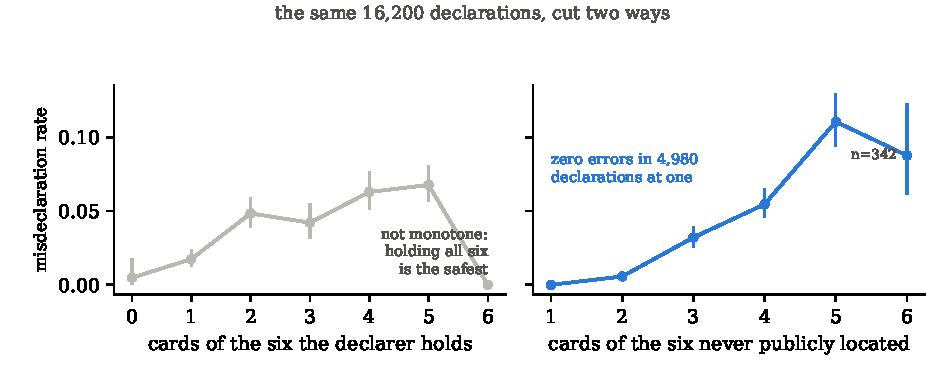
\includegraphics[width=\linewidth]{figs/mediator.pdf}
\caption{The lever everyone reaches for, and the one that carries the risk.
\emph{Left:} misdeclaration rate against how many of the six the declarer
holds. It is not even monotone --- holding all six is the safest state there
is, so the curve turns over at the right-hand end, and any policy tuned on this
covariate is tuned on a confound. \emph{Right:} the same declarations against
how many of the six have \emph{never been publicly located}. That one runs from
zero errors in $4{,}980$ declarations up to eleven percent. The dip at six is
$30$ errors in $342$ declarations and its interval covers the point before it.
Bars are $95\%$ Wilson intervals, which is why the zero cell has a visible
upper limit rather than a degenerate one.}
\label{fig:mediator}
\end{figure}

\begin{figure}[t]
\centering
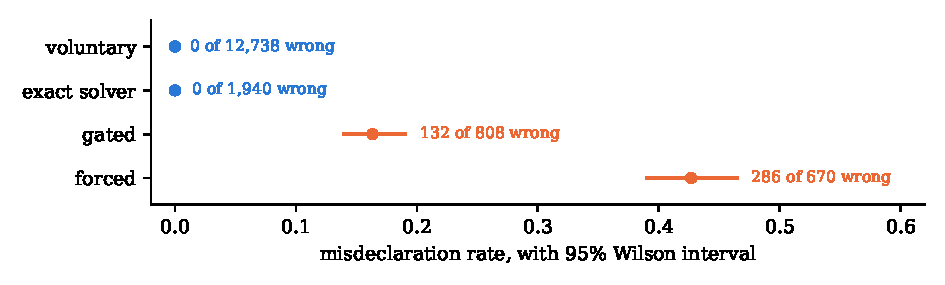
\includegraphics[width=\linewidth]{figs/paths.pdf}
\caption{Every misdeclaration this engine makes is compelled. Split by the path
the declaration arrived on: the two paths it takes because it \emph{wants} to
are exactly perfect over $14{,}678$ declarations between them, and both paths
where it declares because it \emph{must} --- the endgame gate, and a forced
declaration with no cards left to ask with --- carry the whole error rate.
This is why the headroom in \S\ref{sec:missing} is not a calibration problem.
The policy already declines every declaration it is entitled to decline.}
\label{fig:paths}
\end{figure}

\paragraph{What the declaration is actually risking, and a lever that looked
free and was not.} Of our $0.1759$ wrong declarations a game, $0.1676$ are
allocation class --- our own team held all six and we named the wrong split ---
against $0.0083$ ownership errors. That is $95.3\%$, and it is a different
problem from reading the opposition: every card is held by someone who knows
they hold it, so the team has the answer and no member of it does.

The obvious lever is that a declaration may be made by any member of the team,
on their own turn. Someone holding four of the six guesses two; someone holding
one guesses five. Over $1{,}800$ self-play games and $16{,}156$ wholly-held
declarations, $30.4\%$ were made by a player a teammate could have
out-informed, so the opportunity is real. The lever is not:

\begin{table}[t]
\centering
\small
\begin{tabular}{lrrlrr}
\toprule
declarer's own cards & $n$ & error & & $n$ & error \\
\midrule
1 & $2{,}640$ & $0.017$ & \emph{cards never located}: 1 & $4{,}980$ & $0.000$ \\
2 & $2{,}024$ & $0.048$ & \hspace{1em} 2 & $4{,}234$ & $0.006$ \\
3 & $1{,}282$ & $0.042$ & \hspace{1em} 3 & $2{,}990$ & $0.032$ \\
4 & $1{,}494$ & $0.063$ & \hspace{1em} 4 & $2{,}344$ & $0.055$ \\
5 & $1{,}830$ & $\mathbf{0.068}$ & \hspace{1em} 5 & $1{,}266$ & $\mathbf{0.111}$ \\
6 & $6{,}468$ & $0.000$ & \hspace{1em} 6 & $342$ & $0.088$ \\
\bottomrule
\end{tabular}
\caption{The declarer-holding lever against the mediator, on the same $16{,}156$ wholly-held declarations. \emph{Left:} error rate by how many of the six the declarer holds --- the lever, which is not monotone and peaks at five. \emph{Right:} by how many have never been publicly located, which is what the risk actually tracks. Figure~\ref{fig:mediator} plots both with intervals.}
\label{tab:mediator}
\end{table}

The error rate \emph{rises} with the declarer's own holding, so deferring to
the better-placed teammate would move declarations up that curve. Six is
trivially perfect --- hold every card and there is nothing to name.

The right variable is on the right, and it is selection that connects them. A
player holding one card of a half-suit only declares it when the other five are
already pinned; holding five leaves exactly one card unaccounted for, and if
that card was dealt and never asked for it is a coin flip between two teammates
on a set that feels certain. Held at fixed ``never publicly located'' the
$k$-effect flattens: in the best-populated stratum ($4$ unlocated, $n=2{,}344$)
the error rate across $k = 0 \ldots 5$ runs $0.050$, $0.068$, $0.057$, $0.057$,
$0.042$, $0.077$, with no trend. \textbf{What a declaration risks is not how
many cards you are missing but how many of them have never moved.}

\paragraph{And the split is not frozen, which we asserted before checking.}
It is natural to say that once a team holds all six no opponent may legally ask
in the half-suit, so nothing further can inform the split. The first clause is
right and the conclusion does not follow. Hand counts are public and
\texttt{fish/beliefs.py::\_propagate} uses them: a player whose quota reaches
zero is excluded from every unresolved card, and a player whose quota equals
what they could still be holding has those cards pinned. So the split keeps
resolving after it freezes --- not through anything happening in that half-suit,
but through the rest of the game draining hands.

Measured, over the same corpus, as cards pinned to a specific player beyond the
declarer's own hand and beyond anything a successful ask publicly located:
$46.6\%$ of wholly-held declarations derive nothing, $33.2\%$ derive one card,
$15.1\%$ two, $5.1\%$ three or more. $8{,}626$ of $16{,}156$ wholly-held declarations --- $53.4\%$ --- carry at
least one derived card, and the error rate falls from $0.046$ with none to
$0.011$ with one and $0.000$ with three. \textbf{Deriving cards after the
freeze is the common case, not the exception.} It is what makes a declaration safe.
The doomed-ask gate had already implied as much and we read it the other way:
it deferred $0.224$ declarations a game while adding only $0.084$ forced ones,
so about $0.14$ moved into a \emph{confident} declaration, which is only
possible if waiting supplied something.

\paragraph{Is that where the headroom is, though?} The paragraphs above say
where our \emph{errors} are. Those are not the same question, and the
difference is settleable by handing a seat information it should not have and
seeing what it does with it.

\begin{figure}[t]
\centering
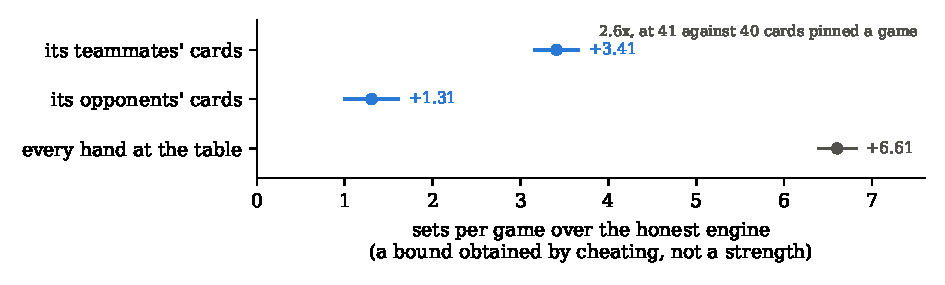
\includegraphics[width=\linewidth]{figs/ceiling.pdf}
\caption{What perfect card-reading is worth, one side of the table at a time.
\textbf{Every value here is obtained by cheating}: the arm is handed the true
deal and the opposition never is, so these bound what information could buy and
are not strength measurements. They never appear in a ladder. The two partial
arms are told almost exactly the same \emph{number} of cards --- $40.7$ against
$40.4$ a game --- and the teammate side is worth $2.6\times$ the opponent side
anyway. We predicted the reverse. The two do not sum to the whole
($4.72$ against $6.61$), so the sides are complements rather than separable
contributions.}
\label{fig:ceiling}
\end{figure}

\textbf{Every figure in this paragraph is a bound obtained by cheating.} The
arms are \path{fish4/oracle.py} handed the true deal; the opposition never
cheats. They are not strength measurements, they do not belong in a ladder, and
they must not be read beside an honest margin. Over $600$ games per arm on
identical deals (\path{prereg/information_ceiling_split.md} $\rightarrow$
\path{results/ceiling_split.json}):

\begin{center}
\small
\begin{tabular}{lrrr}
\toprule
told the true location of & cards pinned/game & ceiling over honest & \\
\midrule
its \textbf{teammates'} cards & $40.7$ & $+3.4100$ & $[+3.1625, +3.6575]$ \\
its \textbf{opponents'} cards & $40.4$ & $+1.3067$ & $[+1.0070, +1.6063]$ \\
everything & $59.8$ & $+6.6067$ & $[+6.4004, +6.8129]$ \\
\bottomrule
\end{tabular}
\end{center}

The middle column is the point. The two partial arms are told \emph{almost exactly
the same number of cards} and one is worth $2.6$ times the other, so this
controls for how much a seat knows and isolates what it knows about. The
allocation/ownership split in the error ledger does translate into a split in
information value, and the answer to the question in this paragraph's title is
yes.

Two cautions, both of which the pre-registration owes the reader. The teammate
arm's zero allocation errors are \emph{definitional} --- a seat that knows every
teammate's cards and its own reads the split off rather than inferring it, so
that cell could not have come out any other way and confirms nothing. And the
arms are sub-additive, $+4.7167$ against $+6.6067$ for omniscience, where the
registration braced for the opposite: knowing where a card is \emph{not} pays
only if you can also act on it.

% =====================================================================
\section{What did not work}
\label{sec:negative}

\subsection{Everything else we tried}
\label{sec:res-null}

Table~\ref{tab:nulls} is the rest of the study. It is mostly nulls, and it is
reported in full because a table of only the things that worked would
misrepresent how much was tried. Each cell is a duplicate-deal duel against the
champion with exactly one thing changed, and the last column is the smallest
effect that cell could have resolved at 80\% power given a per-pair standard
deviation of 3.869 sets.

That column uses one standard deviation for every row, and we now know it is a
property of the comparison rather than of the game. Since the correction is
conservative --- the constant is the noisiest case --- it can only have made
these cells look \emph{less} informative than they were, which raises the
question of whether any of them was in fact resolvable. Rescoring each cell that
stored its per-pair differentials against its own measured noise moves the
resolvable effect by a median factor of $0.92$, and by $0.60$ in the quietest,
and changes no verdict at all.

That last clause was where we stopped, and it was the wrong check. ``$|{\rm
est}| > {\rm MDE}$'' is a test at $\alpha \approx 0.005$, because the MDE is
$(z_{0.975} + z_{0.80})\,\mathrm{se} = 2.80\,\mathrm{se}$; everywhere else in
this paper a cell is said to have resolved something when its \emph{95\%
interval excludes zero}, which is $1.96\,\mathrm{se}$. We had been auditing the
table against a bar $43\%$ higher than our own definition, and since the gap
between the two MDEs is a median $5\%$ of the MDE, finding no change was close
to arithmetically guaranteed.

Under the definition the rest of the paper uses, \textbf{five cells change}: the
retake penalty at $-0.340\ [-0.663, -0.017]$, a decisive lookahead cell at
$+0.307$, and three blocks of pre-registered runs. All five sit below the MDE
their row quotes and have intervals excluding zero. The MDE column says what a
cell could \emph{detect} at $80\%$ power, which is a stricter and different thing
from what it did \emph{resolve}, and reading the column as ``this cell found
nothing'' understates them. The retake cell is the sharpest case: another
pre-registration in this study treats that $-0.340$ as an established effect and
designs a follow-up against it, while this table files it as a null. Both
readings cannot be right, and the interval is the one that governs.

None of this widens a published interval --- each cell's interval was always
computed from its own sample variance, and the constant only ever fed the MDE
column. What it corrects is how that column should be read. The cells that
recorded only a mean and an interval cannot be re-examined at all, which is
itself the argument for storing per-pair data, and why v0.4 does.

\begin{table}[t]
\centering
\small
\begin{tabular}{llrrl}
\toprule
what changed & setting & pairs & set diff & 95\% CI \\
\midrule
\multicolumn{5}{l}{\emph{inference precision}}\\
draws per decision & 96 (from 160) & 160 & $-0.300$ & $[-0.852, +0.252]$ \\
draws per decision & 320 (from 160) & 200 & $-0.035$ & $[-0.578, +0.508]$ \\
count mode & $\sqrt{\cdot}$, $\gamma{=}0.70$, 160 & 200 & $+0.480$ & $[-0.042, +1.002]$ \\
count mode & $\sqrt{\cdot}$, $\gamma{=}0.70$, 320 & 200 & $-0.165$ & $[-0.701, +0.371]$ \\
no-declaration signal$^\dagger$ & $\lambda = 0.9$ & 200 & $+0.205$ & $[-0.301, +0.711]$ \\
no-declaration signal$^\dagger$ & $\lambda = 1.8$ & 200 & $+0.190$ & $[-0.313, +0.693]$ \\
\midrule
\multicolumn{5}{l}{\emph{new ask-objective terms}}\\
exposure & $0.40$ & 160 & $-0.113$ & $[-0.660, +0.435]$ \\
claim progress & $0.30$ & 160 & $-0.206$ & $[-0.807, +0.395]$ \\
signalling & $+0.25$ & 160 & $-0.300$ & $[-0.890, +0.290]$ \\
signalling & $-0.25$ (conceal) & 160 & $+0.056$ & $[-0.530, +0.642]$ \\
information gain & $0.10$ & 160 & $-0.394$ & $[-0.932, +0.144]$ \\
concentration$^\ddagger$ & $0.15$ & 160 & $-0.037$ & $[-0.653, +0.578]$ \\
turn-risk retune & $0.35$ (from $0.60$) & 160 & $-0.075$ & $[-0.670, +0.520]$ \\
scarcity retune & $0.35$ (from $0.20$) & 160 & $+0.125$ & $[-0.381, +0.631]$ \\
\midrule
\multicolumn{5}{l}{\emph{claiming and the endgame}}\\
claim threshold & $0.99$ (from $0.97$) & 200 & $+0.010$ & $[-0.010, +0.030]$ \\
informed pass choice & on & 160 & $+0.013$ & $[-0.012, +0.037]$ \\
tablebase & one half-suit only & 200 & $+0.005$ & $[-0.005, +0.015]$ \\
tablebase & disabled entirely & 200 & $+0.005$ & $[-0.005, +0.015]$ \\
\midrule
\multicolumn{5}{l}{\emph{the learned half-suit value objective}}\\
blended & $w_{\mathrm{value}} = 0.5$ & 200 & $+0.410$ & $[-0.086, +0.906]$ \\
blended & $w_{\mathrm{value}} = 1.5$ & 200 & $+0.040$ & $[-0.502, +0.582]$ \\
\textbf{replacing the objective} & pure $\Delta V$ & 200 & $\mathbf{-7.355}$ & $[-7.875, -6.835]$ \\
\bottomrule
\end{tabular}
\caption{Everything else. Only the last row resolves, and it resolves against
us. Every other interval contains zero at a minimum detectable effect of
roughly $0.8$ sets per pair, so these are ``not shown to matter at this budget'',
not ``shown not to matter''.}
\label{tab:nulls}
\end{table}

Four of these deserve comment.

$^\ddagger$\,\textbf{This row is retained as history and does not describe the
code.} Both halves of it were incapable of finding an effect, and the reason is
worth more than the row.

The \emph{formula} could not express the preference it was written for.
\texttt{concent} at v1 was \texttt{ctx.team\_concentration[hs]}: one number per
half-suit, identical for every candidate ask in it and independent of the
target and of who would end up holding the card. A term taking the same value
on every ask in a half-suit can tilt the choice of half-suit and nothing else.
Worse, its sign is backwards in the case it exists for --- when the
concentration sits with a \emph{teammate}, taking a card breaks it up, and v1
scored that ask highest precisely because the half-suit was concentrated. This
is the defect \texttt{claim} carried at v1, and it takes the same remedy:
corrected in place to the expected \emph{change} the ask would cause, with
\texttt{TERM\_VERSIONS["concent"]} bumped to $2$ so that
\texttt{stale\_terms()} flags every stored harvest fitted against the old
column.

And the \emph{weight} was inert. Measured over $596$ decisions with a real
choice and $30{,}065$ candidate asks
(\path{scripts4/concent_scale.py} $\rightarrow$
\path{results/concent_scale.json}), the corrected feature has median magnitude
$0.0299$ and a median within-decision spread of $0.0677$. At the screened
weight of $0.15$ it changes which ask is taken on $1.7\%$ of decisions; it
takes a weight near $1.0$ to reach $8\%$. A $160$-pair run of a knob acting on
one decision in sixty, reporting an interval four times the ship bar in each
direction, is a statement about the harness rather than about the idea.

The retest mattered because this is the only term in the basis that points at
the error we actually make. Of our $0.1759$ wrong declarations a game, $0.1676$
are allocation class --- our own team held all six and we named the wrong split
--- against $0.0083$ ownership errors, and a half-suit held entirely in one
hand has no split to name. It was registered at
\path{prereg/concentration_v2.md} at $4{,}000$ games, with arms at $0.60$ and
$1.50$ and with the mechanism as a \emph{withdrawal condition} rather than a
secondary: allocation errors had to fall and concentration at declaration time
had to rise.

\textbf{It ran and it is withdrawn, on condition 1.} At $w = 0.60$ the effect is
$-0.0430$ $[-0.1369, +0.0509]$ and at $1.50$ it is $-0.1445$ $[-0.2490,
-0.0400]$, worse than shipped. Allocation errors were required to fall and rose
monotonically instead: $0.1557$, $0.1772$, $0.1827$. Condition 2 passed ---
concentration really did rise, $0.8106 \to 0.8168$ --- so the corrected feature
computes what it claims and the \emph{strategy} is what is wrong, which is a
more useful outcome than a null.

The reason is the resource the argument for the term ignored.
\texttt{GameState.legal\_asks} requires the asker to hold a card of the
half-suit, so concentrating a team's holding into one hand narrows the set of
half-suits that hand can ask in --- and being unable to ask is the definition of
being forced. Forced declarations rise monotonically with the weight, $0.167 \to
0.197 \to 0.218$ a game, and the forced path is $47$--$49\%$ wrong. The term
buys a marginally better split and pays for it in the one currency that keeps a
seat able to act. (Stated as consistent-with rather than proven: the run does
not instrument askable half-suits per seat, and the monotone dose response in
the harm is the strongest evidence here.)

$^\dagger$\,\textbf{These two rows measured nothing, and we found out
afterwards.} The no-declaration term was assembled into the importance weights
and then overwritten: the batch sampler built it first and the opponent-model
branch that follows did \texttt{logl = } rather than \texttt{logl += }, so
whenever any non-self player had already asked --- $632$ of $641$ decisions in
\path{results/ess_probe.json} --- the term was discarded before use. In the
handful of decisions where it survived, it addressed the half-suit by column
indices built against the caller's free-card order and applied to a matrix whose
columns are in the sampler's own sort; six of eight columns differ on a typical
position, so the ``did the opponents take this whole half-suit'' test read a
mixture of cards from other half-suits. And the scalar reference sampler stored
the term and never applied it at all, so the batch/scalar agreement test could
not see any of this.

Both cells are therefore reported as \emph{invalid rather than null}: they are
what a disabled feature scores, which is the champion plus sampling noise, and
the intervals above are consistent with exactly that. All three bugs are fixed
and pinned by tests that fail against the previous code; the feature has not
been re-measured, and until it is there is no result here in either direction.
Nothing else in this paper is affected, because \texttt{opp\_lambda} defaults to
zero and no other cell sets it.

\textbf{Precision appeared to have saturated, and it had not.} v0.3 found that
raising the sampled-world count from 32 to 96 was worth $+0.54$ sets per pair
and concluded that belief precision had not saturated. Under v0.4's inference
these screens said it plainly had: halving or doubling the draw budget around
$160$ changed nothing measurable, and the natural reading was that v0.3 had been
buying accuracy rather than precision --- more draws partially averaging out a
\emph{bias} --- so that once the bias was gone, sampling noise was no longer
binding.

\textbf{That reading is refuted}, by a pre-registered $6000$-pair run reported
in Section~\ref{sec:res-precision}: going from $160$ draws to $480$ is worth
$\mathbf{+0.340}$ sets per deal-pair, $95\%$ CI $[+0.243, +0.436]$, all six
blocks positive, $I^2 = 0\%$. Precision had not saturated; the screens that said
so were $200$-pair cells resolving about $\pm 0.53$, which cannot distinguish
$+0.340$ from zero and returned exactly the null they were bound to return.
Their agreement with each other was not corroboration --- underpowered cells
agree on nothing in particular, and four of them agreeing on a null is what four
underpowered cells do. The paragraph is kept in its original form above because
the inference it drew was reasonable on the evidence available and wrong anyway,
which is this paper's most frequently repeated lesson and is more useful stated
against a concrete case than in the abstract.

The word was right and the rung was wrong, which is the more interesting
correction. A second pre-registered run at $480 \to 1440$ draws returns
$+0.094$ $[-0.002, +0.191]$, and the contrast against rung 1's $+0.340$ is
$-0.245 \pm 0.069$ --- so precision's returns \emph{do} diminish, just not
where the screens said. Saturation has not begun at $160$ and has begun by
$480$. See Section~\ref{sec:res-precision}.

\textbf{One cell technically resolves, and should still be ignored.} Lowering
the claim bar from $0.97$ to $0.90$ gives $+0.035$ $[+0.007, +0.063]$: an
interval excluding zero, and an effect of one fortieth of a set per deal-pair.
After forty-odd cells at a nominal 95\% level, an interval that narrowly
excludes zero at a magnitude this small is not evidence of anything, and we
report it rather than promoting it --- particularly having already watched a
larger apparent effect fail to replicate twice
(Section~\ref{sec:res-replication}). The neighbouring cell in the other
direction ($0.99$) gives $+0.010$ $[-0.010, +0.030]$, which is the shape of a
policy that barely changes its decisions at all. This one has since been run
properly, and Section~\ref{sec:res-claimthreshold} reports what an unselected
2000 pairs did to it.

\textbf{The claim threshold and the tablebase are exact no-ops.} The intervals
$[-0.010, +0.030]$ and $[-0.005, +0.015]$ are not small effects; they are almost
no divergence at all. Raising the claim bar from $0.97$ to $0.99$ changes
essentially no decisions, reproducing v0.3's bimodality finding on a much better
posterior. Disabling the exact endgame solver entirely changes essentially
nothing, which agrees exactly with the absolute benchmark
(Section~\ref{sec:res-absolute}), where it changed not one of 988 decisions.

\textbf{Replacing the objective with the learned value is catastrophic.} The
half-suit value model is good --- held-out log-loss $0.727$ against $0.821$ for
the class prior and $0.743$ for the best single feature, and a mean calibration
bias of $-0.006$. That last figure flatters it, and the flattery is worth one
sentence because ``well-calibrated'' is doing work in the argument below. Five
of its ten deciles are miscalibrated at the $95\%$ level: it is over-confident
at both ends (decile 0 says $7.6\%$ and delivers $0.5\%$; decile 9 says $92.7\%$
and delivers $90.0\%$) and under-confident in the middle (deciles 4 and 5 both
run about $3$ points high). The mean bias is near zero because those errors
cancel, not because each decile is right. Scoring asks by the expected change in
it, in units of sets, loses $7.4$ sets per deal-pair. Blending it in at low
weight is harmless and does nothing. This is the sharpest confirmation of v0.3's
central claim about this game that we have: the probability that an ask lands is
not one term among several, it is the objective, and a decently-calibrated model of
what a half-suit is worth is no substitute for it.

\textbf{The eleven-term basis bought nothing.} Neither the two terms motivated
by the literature survey (exposure, signalling) nor the four motivated by
inspection improved on v0.3's three. The signalling term is worth singling out
because its sign was the interesting question: $+0.25$ (advertise a holding in a
half-suit our team is winning) scored $-0.300$ and $-0.25$ (conceal it) scored
$+0.056$, so if anything the concealment direction is favoured, but neither
interval comes close to excluding zero.

\subsection{The near-misses, and the one that resolved}
\label{sec:res-replication}

Two cells in Table~\ref{tab:nulls} had positive point estimates whose intervals
only just included zero, which is exactly the situation in which a screening
study manufactures a false positive if the best cell is promoted without
re-measurement. We reran both at 500 pairs on fresh seeds --- minimum detectable
effect $0.48$ rather than $0.77$ --- together with their combination:

\begin{center}
\small
\begin{tabular}{lrrl}
\toprule
candidate & screen (200 pairs) & retest (500 pairs) & retest 95\% CI \\
\midrule
blended value objective, $0.5$ & $+0.410$ & $-0.208$ & $[-0.534, +0.118]$ \\
$\sqrt{\cdot}$ counting, $\gamma = 0.70$ & $+0.480$ & $+0.212$ & $[-0.092, +0.516]$ \\
\textbf{both together} & --- & $\mathbf{+0.490}$ & $\mathbf{[+0.184, +0.796]}$ \\
\quad replication, fresh seeds & --- & $+0.068$ & $[-0.254, +0.390]$ \\
\quad replication again & --- & $-0.066$ & $[-0.395, +0.263]$ \\
\bottomrule
\end{tabular}
\end{center}

When this was written the combination was the only cell in the study --- out of
more than twenty-five --- whose interval excluded zero in the improvement
direction, which is exactly why it looked like something. On a fresh set of 500
deals it returned $+0.068$, and on a second fresh set $-0.066$. It was noise.

That framing no longer holds, and the reason it stopped holding is the point.
Three cells in this paper now exclude zero upward --- the pre-registered
lookahead at $+0.104$, posterior precision at $+0.340$ and at-ask depth at
$+0.102$ --- and every one of them was \emph{designed} to be able to, at thirty
times this cell's sample size with the analysis fixed in advance. The
distinction that matters is not how many intervals clear zero, it is whether
clearing zero was a possible outcome of a design or the best of twenty-five
looks.

An earlier draft of that sentence said \emph{four}, and counted the claim
threshold's $+0.035$ among them. That was the error the sentence is about,
committed inside the sentence about it: the claim-threshold figure is a
screening cell selected out of $103$ for excluding zero, which is the
\emph{other} category entirely. It is the eighth appearance of the pattern
this paper keeps documenting, the fourth of them one level above where the
error was last caught, and the only one caught by a \emph{run} rather than by
rereading --- the confirmatory 2000 pairs of
Section~\ref{sec:res-claimthreshold} put the effect at $+0.002$.

We report this at length because it is the single most useful methodological
observation the study produced. Twenty-five screening cells at a nominal 95\%
level will produce roughly one apparent winner under a complete null, and this
one arrived with a respectable-looking interval, a plausible story (two
independently-motivated changes that stack, exactly as v0.3's two winning terms
had) and a point estimate twice the sum of its parts --- which should have been
the tell. Promoting it would have shipped a change worth nothing and, worse,
would have anchored the next version's baseline on it.

% =====================================================================
\section{Search over the belief, measured}
\label{sec:searchres}

\subsection{Belief-space search: four rounds to one answer}
\label{sec:res-lookahead}

Section~\ref{sec:lookahead} describes the one search design the variance
diagnosis does not rule out, and predicts, in Proposition~\ref{prop:greedy},
that a version of it without the quota coupling would collapse to greedy. Both
halves were measured. Table~\ref{tab:lookahead} is the whole record, and it took
9{,}700 deal-pairs across four rounds --- 800 in screens, 1500 in replications,
1400 decisive, 6000 in the pre-registered settling run --- to answer a question
a 200-pair cell appeared to answer at the start.

The answer is that the search helps, by about a tenth of a set per deal-pair.
The section is long because the route to that number is the more useful part:
the first cell overstated it by a factor of five, the next three rounds
disagreed with each other, and the disagreement turned out to be a fact about
selection rather than about the harness or the game.

% BEGIN lookahead-table (generated by scripts4/lookahead_table.py --write)
\begin{table}[t]
\centering
\small
\begin{tabular}{lrrlr}
\toprule
cell & pairs & set diff & 95\% CI & MDE \\
\midrule
depth 3, $w=0.25$ & 200 & $\mathbf{+0.570}$ & $[+0.125, +1.015]$ & 0.75 \\
depth 2, $w=0.25$ & 200 & $+0.345$ & $[-0.083, +0.773]$ & 0.75 \\
depth 3, $w=0.60$ & 200 & $-0.080$ & $[-0.583, +0.423]$ & 0.75 \\
depth 3, \emph{no quota coupling} & 200 & $+0.070$ & $[-0.369, +0.509]$ & 0.75 \\
\midrule
depth 3, $w=0.25$ --- retest & 500 & $-0.044$ & $[-0.321, +0.233]$ & 0.48 \\
\midrule
\quad --- retest again & 500 & $\mathbf{+0.386}$ & $[+0.086, +0.686]$ & 0.48 \\
\midrule
\emph{no coupling} --- retest & 500 & $+0.112$ & $[-0.164, +0.388]$ & 0.48 \\
\midrule
depth 3, $w=0.25$ --- decisive A & 700 & $\mathbf{+0.307}$ & $[+0.063, +0.551]$ & 0.40 \\
\midrule
\quad --- decisive B & 700 & $+0.001$ & $[-0.240, +0.243]$ & 0.40 \\
depth 3, $w=0.25$ --- settle, block 1 & 1000 & $+0.179$ & $[-0.034, +0.392]$ & 0.34 \\
\quad --- block 2 & 1000 & $-0.009$ & $[-0.217, +0.199]$ & 0.34 \\
\quad --- block 3 & 1000 & $+0.118$ & $[-0.089, +0.325]$ & 0.34 \\
\quad --- block 4 & 1000 & $\mathbf{+0.241}$ & $[+0.040, +0.442]$ & 0.34 \\
\quad --- block 5 & 1000 & $+0.064$ & $[-0.147, +0.275]$ & 0.34 \\
\quad --- block 6 & 1000 & $+0.028$ & $[-0.175, +0.231]$ & 0.34 \\
\bottomrule
\end{tabular}
\caption{Belief-space lookahead against the v0.4 champion, which is the identical policy with the bonus disabled. MDE is the smallest effect that cell could have resolved at 80\% power, so a null row says the run did not detect an effect of that size, not that there is none. This table uses the per-pair standard deviation of $3.796$ measured over the 4800 A/A pairs reported later in this section, rather than the $3.869$ used elsewhere in this paper: the settling run was powered against $3.796$, and a table reporting a run against a different resolution from the one it was designed for would misstate what it could see. The two differ by under $2\%$.}
\label{tab:lookahead}
\end{table}
% END lookahead-table

\paragraph{Three runs of one configuration disagree.} The screening cell, at 200
pairs, returned $+0.570$ and excluded zero. Following the replication policy of
Section~\ref{sec:res-replication} we reran the identical configuration twice
more at 500 pairs, changing nothing but the seed streams. The two retests
returned $-0.044$, 95\% CI $[-0.321, +0.233]$, and $+0.386$, 95\% CI
$[+0.086, +0.686]$. The second of those excludes zero. The first does not, and
its interval excludes the value the second reports.

That is not a result about the lookahead. It is a result about the experiment.
Three estimates of one quantity, differing only in seeds, are mutually
inconsistent: Cochran's $Q = 7.03$ on 2 degrees of freedom, $p = 0.030$, with
$I^2 = 71.5\%$ --- so roughly seven-tenths of the spread between these runs is
\emph{not} the sampling variation their own intervals model.

\paragraph{The within-run intervals are not the problem.} The per-pair standard
deviation recovered from each cell separately is $3.21$, $3.17$ and $3.42$ sets.
Those agree with each other and with the $3.869$ figure used throughout this
paper, so each interval correctly describes the deals that run actually played.
The natural inference is that the variance the intervals miss sits \emph{between}
runs; the DerSimonian--Laird estimate of such a component from these three cells
is $\tau = 0.268$ sets per deal-pair. \emph{We measured that inference directly
and it is wrong} --- see below --- but it is worth following through first,
because the two pooled answers it produces are the reason the question mattered
enough to measure.

Pooling all 1200 pairs on that assumption gives two answers, and only one of
them is usable:
\begin{center}
\begin{tabular}{lll}
\toprule
pooling & estimate & \\
\midrule
fixed effect   & $+0.226$ $[+0.041, +0.411]$ & excludes zero \\
random effects & $+0.278$ $[-0.083, +0.638]$ & includes zero \\
\bottomrule
\end{tabular}
\end{center}
A fixed-effect pool assumes the runs are three samples of one true value, which
is precisely what $Q$ appears to reject; the random-effects interval, which adds
$\tau^2$ to every cell, would then be the one reflecting where a fourth run might
land, and it includes zero. Read that way the effect is unresolved and could be
reported neither as working nor as a null --- which is where we left it, and
which is what made the size of $\tau$ worth establishing rather than assuming.

\paragraph{The three cells prompted a question about the harness, and the
answer is that the harness is fine.} The reading above --- that a duplicate-deal
cell has a variance component its own interval does not model --- would, if true,
make the minimum-detectable-effect table of Section~\ref{sec:eval} optimistic for
every single-cell result in this paper. That is too consequential to leave
inferred from three points, so we measured it.

The instrument is an \textbf{A/A}: one policy against a copy of itself, where the
true differential is exactly $0$. That required a change to the harness, and the
reason is worth recording, because it means this question could not previously
have been asked. Under the default seat-based seeding an A/A plays a
bit-identical game in both halves of a duplicate pair, so its differential is
$(a-b) + (b-a) = 0$ for every deal --- a point mass, not a small effect correctly
measured as zero. The harness could not observe its own null. Giving each side an
independent randomness stream (\texttt{independent\_seeds}, off by default so the
archive stays comparable) makes the null a real random variable.

Twenty-four blocks of 200 pairs, each with its own deal seeds and its own agent
seeds --- differing in exactly the way two separate runs differ:

\begin{center}
\begin{tabular}{lr}
\toprule
nominal 95\% intervals covering the truth & $23/24 = 95.8\%$ \ \ $[79.8, 99.3]$ \\
Cochran's $Q$ & $18.41$ on 23 df, $p = 0.735$ \\
$I^2$ & $0.0\%$ \\
$\tau$, between-run standard deviation & $\mathbf{0.0000}$ \\
grand mean of the 24 estimates & $-0.0215$ \ (truth: $0$) \\
per-pair standard deviation, 4800 pairs & $3.796$ \ (this paper uses $3.869$) \\
\bottomrule
\end{tabular}
\end{center}

Coverage is nominal. The observed spread of the block estimates, $0.2454$, is
\emph{smaller} than their own standard errors predict, $0.2701$; there is no
excess variance to attribute. A duplicate-deal interval means what it says.

\paragraph{So we retract the between-run variance.} An earlier version of this
section reported $\tau = 0.268$ sets per pair from the three cells above and
argued that it made every small result in this paper more fragile than it looks.
That was a Type I error. The $Q = 7.03$, $p = 0.030$ which produced it is exactly
the one-in-thirty event, and we promoted it to a structural claim about the
harness on the strength of three points --- which is the error this paper devotes
Section~\ref{sec:res-replication} and two of its four lessons to warning against,
committed inside the section doing the warning. The minimum-detectable-effect
table stands as written.

\paragraph{Which leaves the lookahead genuinely open, on better terms.} If the
cells are homogeneous --- and a harness that produces no excess heterogeneity
under the null is strong evidence that they are --- then fixed-effect pooling is
the valid analysis, and over all 1200 pairs the estimate is $+0.226$, 95\% CI
$[+0.041, +0.411]$.

We did not report that as a result. It excludes zero by $0.04$; this
configuration had already produced one screening cell that failed to replicate;
and reaching for the pooling that happens to resolve, immediately after the
pooling that happened not to, is the same error in the opposite direction. So we
fixed a size in advance and ran it: two further cells of 700 pairs each, on fresh
seeds, pre-registered as decisive.

They returned $+0.307$, 95\% CI $[+0.063, +0.551]$, and $+0.001$, 95\% CI
$[-0.240, +0.243]$.

\paragraph{The verdict, on the test we committed to.} Pooled, those two cells
give $+0.153$, 95\% CI $[-0.019, +0.324]$ --- which \emph{includes zero}. The
experiment designed in advance to settle this does not settle it, and we report
that rather than the alternative below, because a post-hoc pool does not get to
overrule a pre-registered one.

\paragraph{What the fuller picture says, and why we still do not claim it.}
Dropping the original screening cell --- it was \emph{selected} for resolving, so
including it in any pooled estimate is winner's curse --- and pooling the four
unselected cells over 2400 pairs gives $+0.153$, 95\% CI $[+0.022, +0.285]$. The
point estimate is identical to three decimal places across both analyses, which
is fairly strong evidence that a small real effect exists, of order a seventh of
a set per deal-pair. It is not evidence that we have demonstrated one.

Dropping that cell also disposes of the heterogeneity this section opened with:
$Q$ falls to $p = 0.063$ over the four unselected cells and $p = 0.081$ over the
two decisive ones, neither significant. Combined with the A/A measurement above,
the story is simply that one cell was selected for being large and the rest is
sampling noise --- no between-run variance, and nothing wrong with the harness.

\paragraph{And the sizing was wrong, by the error this section is about.} We
chose $n = 2600$ on the grounds that its minimum detectable effect of $0.21$
would separate $+0.23$ from zero. But $+0.23$ was the pool \emph{including} the
selected cell --- the inflated estimate. Against the unbiased $+0.153$, a
correctly powered test needs roughly $5000$ pairs. We committed the winner's
curse in the power calculation for the experiment whose purpose was to correct
for the winner's curse, which is the third time in this study the same error has
appeared one level up from where it was last caught. It appears a fourth time in
Section~\ref{sec:res-regret}, inside the estimator built to measure the ask
objective, where taking a maximum over eighteen noisy action values would have
reported two thirds of a set of regret that does not exist. The pattern is worth
naming: each occurrence is not a repetition of the last but a level above it,
and none was caught by being more careful --- each was caught by measuring the
thing that had been reasoned about.

\paragraph{The pre-registered run, and the answer.} So we wrote the analysis
down before running it. \path{jobs/PREREGISTRATION_lookahead.md} fixes, in
advance: six blocks of 1000 fresh pairs; sizing against the \emph{unbiased}
$+0.153$ rather than any figure containing the selected cell; a per-pair
standard deviation of $3.796$ from the A/A rather than the older $3.869$; a
fixed-effect pool of the six new blocks as the only thing that decides; no cell
droppable for its result; and no further run added to chase significance. The
last six rows of Table~\ref{tab:lookahead} are that run.

\begin{center}
\small
\begin{tabular}{lll}
\toprule
& estimate & \\
\midrule
\textbf{primary} --- the six new blocks, 6000 pairs
  & $\mathbf{+0.104}$ $[+0.020, +0.189]$ & \textbf{excludes zero} \\
secondary --- all ten unselected cells, 8400 pairs
  & $+0.119$ $[+0.048, +0.190]$ & excludes zero \\
\bottomrule
\end{tabular}
\end{center}

The effect is demonstrated. Three things belong beside that sentence.

The estimate has fallen at every stage --- $+0.570$ at the screening cell,
$+0.153$ pooled over the unselected cells, $+0.104$ now. That is the
winner's-curse decay in its textbook shape, and the pre-registered figure is the
one with no selection in it.

The run was sized against $+0.153$, whose 80\% power at 6000 pairs needs a true
effect of $0.137$. Against a true $+0.104$ it was under-powered, and the lower
bound of $+0.020$ says how narrowly it cleared. A replication would be worth
more here than another decimal place.

And the heterogeneity that opened this section is gone: $Q = 4.08$ on 5 degrees
of freedom, $p = 0.54$, $I^2 = 0\%$, $\tau = 0$. Six blocks of one configuration
agree within their own intervals, which is what the A/A predicted and what the
original three cells did not. The disagreement really was one selected outlier
and sampling noise.

The implementation shipped disabled while the effect was undemonstrated. On the
strength of the primary test that default can now change --- for a gain of about
a tenth of a set per deal-pair, against the cost measured in
Section~\ref{sec:lookahead-cost}, which is a trade rather than a free win.

\paragraph{What survives regardless.} Proposition~\ref{prop:greedy} does not
depend on any of this. A possession-chain search over a belief whose transition
edits only the asked card's row is exactly greedy at every depth, so the obvious
version of this idea is a no-op by construction rather than by measurement. That
is a structural statement about why search keeps failing in this game, it
removes a whole branch of the design space rather than a point in it, and it is
the part of Section~\ref{sec:lookahead} we would keep. Its empirical shadow is the
no-coupling cell, and the shadow is worth stating carefully, because the
proposition entails greedy equivalence \emph{at a node} and the step from there
to a null set differential is a modelling inference rather than a theorem.
Setting \texttt{couple=False} also does not restore the proposition's hypotheses
outright --- the transition still zeroes the asked row and decrements the
target's count. What is demonstrated is narrower and still to the point. Instrumenting the
search itself over $60{,}277$ multi-branch nodes on champion trajectories
(\path{scripts4/greedy_shadow.py}), the coupled arm departs from the
highest-probability branch at $452$ of them, $0.750\%$; the uncoupled arm
departs at $\mathbf{1}$, $0.0017\%$ --- a factor of $452$. Its set differential
is a null at both 200 and 500 pairs ($+0.070$ and $+0.112$, both intervals
comfortably containing zero), which is consistent with that.

The single uncoupled departure is worth a sentence, because it is real ---
relative gap in $q$ of $1.9\times 10^{-3}$, three orders of magnitude above
floating point --- and Proposition~\ref{prop:greedy} predicts exactly zero. It
is not a contradiction. \texttt{couple=False} does not restore the
proposition's hypotheses, as the module says: the transition still decrements
the target's count, so a player reduced to zero cards drops out of
\texttt{legal\_asks} and the available branch \emph{set} changes downstream.
That is a channel the exchange argument does not cover. The empirical shadow is
therefore a near-null with a mechanism rather than a null, and an earlier draft
reporting it as ``$53{,}273$ of $53{,}273$'' overstated it --- those counts were
in the paper and in no results file, which is how a number stays unchallenged. We would also withdraw a remark from an earlier draft that the
coupling ``changed no decision at all'': over $1{,}110$ champion-trajectory
positions the coupled and uncoupled arms disagree on $0.54\%$ of decisions, so
observing no disagreement in a sample of $59$ is the modal outcome rather than
evidence of equality.

\paragraph{Does it still pay once precision is bought?} The two demonstrated
features of this version --- the belief-space search and the larger posterior
sampling budget --- were each measured against the champion \emph{alone}, so
neither says anything about the other. They could add, or the sharper belief
could already be earning what the search was earning. Pre-registered in
\path{jobs/PREREGISTRATION_stack.md} and written at one of six blocks, which
is the only moment at which writing such a thing proves anything:
\begin{center}
\begin{tabular}{lrl}
\toprule
& set diff & 95\% CI \\
\midrule
lookahead on top of $480$ draws, $6000$ pairs & $+0.072$ & $[-0.010, +0.154]$ \\
\bottomrule
\end{tabular}
\end{center}
Cochran's $Q = 1.94$ on $5$ df ($p = 0.86$), $I^2 = 0\%$, $\tau = 0$ --- the six
blocks agree completely.

The interval contains zero, and the pre-registration fixed in advance how that
must be read. At $6000$ pairs this run has $68\%$ power against the $+0.104$ it
was sized against, so failing to exclude zero is a \emph{failure to resolve an
effect of the size assumed} and is not evidence that the search stops paying.
The script that prints this verdict refuses to print the second sentence. It is
a genuine limit of the design rather than a finding, and the honest summary is
that we do not know.

What the run does bear on is additivity, and only weakly. The search on its own
measured $+0.104$; on top of the sampler it measures $+0.072$, a difference of
$-0.032$ with the two intervals overlapping. As far as this study can tell the
two features add rather than overlap --- with one point on each side of the
comparison, which is exactly as weak a statement as it sounds. Neither
\texttt{WEB\_DRAWS} nor \texttt{V04\_STRONGEST} moves on this result in either
direction: both features are independently demonstrated, and this run is about
what may be \emph{claimed}, not about what ships.

\texttt{w\_lookahead} still defaults to $0$, and that is now a choice about cost
rather than about evidence. The effect is demonstrated; it is worth about a tenth
of a set per deal-pair for roughly $6.7$~ms per decision
(Section~\ref{sec:lookahead-cost}), so a caller under a latency budget should
decide deliberately instead of inheriting. The engine exposes the enabled
configuration under its own name rather than by moving the default, because every
``vs champion'' cell in this paper names the default spec and moving it would
redefine what those runs measured.

% =====================================================================
\subsection{Is the opponent model just fitting its own kind?}
\label{sec:res-robust}

The model is a hypothesis about how opponents choose, and the opponents it was
measured against in Table~\ref{tab:gamma} are copies of the same policy. Two
tests separate a real effect from self-play overfitting.

\begin{table}[t]
\centering
\small
\begin{tabular}{llrrl}
\toprule
opponent & agent & pairs & set diff / pair & 95\% CI \\
\midrule
\multirow{2}{*}{\texttt{memory} (off-distribution)}
  & $\gamma = 0.30$ & 150 & $+4.727$ & $[+4.119, +5.335]$ \\
  & $\gamma = 0$    & 150 & $+3.793$ & $[+3.247, +4.340]$ \\
\midrule
\multirow{2}{*}{anti-model exploiter}
  & $\gamma = 0.30$ & 200 & $+6.570$ & $[+6.113, +7.027]$ \\
  & $\gamma = 0$    & 200 & $+5.735$ & $[+5.237, +6.233]$ \\
\bottomrule
\end{tabular}
\caption{The opponent model against opponents it was not shaped by.
\texttt{memory} acts only on facts it can prove and has no probabilistic
component at all. The anti-model exploiter is the v0.4 policy with the depth
term \emph{inverted} ($w_{\mathrm{suit}} = -0.35$), so it deliberately asks in
half-suits it is shallow in --- the exact behaviour the model assumes does not
happen.}
\label{tab:robust}
\end{table}

Against \texttt{memory}, a policy with no probabilistic component whatsoever,
the model is still worth about $+0.93$ sets per pair. Against an opponent built
specifically to violate its assumption it is still worth about $+0.84$. The
second number deserves care: the exploiter is a weak policy in absolute terms
(inverting the depth term costs it a great deal), so what the comparison shows
is that the model is not \emph{harmed} by an opponent designed to mislead it,
not that it cannot be exploited by a stronger adversary. A genuinely coordinated
best-responder is future work.

\subsection{Does it survive the rule variants?}
\label{sec:res-rules}

The engine supports several rule options, and a result that only holds under one
configuration is a weaker result. Table~\ref{tab:rules} repeats the headline
comparison under three of them. One row has since changed status: the games
of this section were played under the void-era misdeclaration default, so
``wrong split $\to$ opponents'' was a variant when it was measured --- it is
now the baseline (\S\ref{sec:game}), and the row is the measurement the rule
correction's continuity expectation was registered against. Its $+1.690$
carries one caveat worth stating: both agents' declaration policies at the
time still priced misses with void-era expected values, so the row shows the
margin survives the rule, not that either side played it optimally --- the
restated headline under the award baseline, with both sides pricing it
correctly, is design R1 of \path{prereg/rules_award_baseline.md}.

\begin{table}[t]
\centering
\small
\begin{tabular}{llrrl}
\toprule
rule & comparison & pairs & set diff & 95\% CI \\
\midrule
declare at any time & v0.4 vs v0.3 champion & 200 & $+2.175$ & $[+1.647, +2.703]$ \\
declare at any time & $\gamma$ vs no $\gamma$ & 200 & $+1.935$ & $[+1.450, +2.420]$ \\
48-card deck & v0.4 vs v0.3 champion & 200 & $+1.080$ & $[+0.557, +1.603]$ \\
wrong split $\to$ opponents & v0.4 vs v0.3 champion & 200 & $+1.690$ & $[+1.191, +2.189]$ \\
\bottomrule
\end{tabular}
\caption{The result holds under every rule variant tested, including the
declare-at-any-time rule as the game is usually written down. Note the 48-card
row: with eight half-suits instead of nine, the margin roughly halves, which is
what one would expect if the advantage is inferential --- a smaller deck leaves
less to infer.}
\label{tab:rules}
\end{table}

The declare-at-any-time rows required an engine change. v0.3's game loop only
ever asked the player on move, so although the rule was accepted by the
configuration it could not be exercised by any policy --- and it matters most
precisely where it is unreachable, for a seat that has run out of cards and
therefore never gets a turn of its own while a teammate still has some. v0.4
polls off-turn seats for a claim they can make \emph{by deduction alone}, which
costs a belief update rather than a posterior per seat, and offers it identically
to both generations so that the comparison stays a comparison of one thing.

% =====================================================================
\section{Learning the objective from data}
\label{sec:learnres}

\subsection{Learning the ask objective}
\label{sec:res-learn}

v0.3's stated top priority for this version was to learn the ask objective
rather than hand-weight it. We did, by common-random-numbers paired rollout
regression: 874 positions, 83{,}168 games played to the end, all pairs of
candidate asks within a position regressed on the difference of their feature
vectors, with standard errors clustered by position (the naive standard errors
are on average $2.00\times$ too small, since pairs from one position share
candidates, worlds and rollout seeds).

The machinery works: common random numbers cut the variance of a pairwise
comparison to $0.64$ of independent worlds, bringing the noise-to-signal ratio
from v0.3's $2.4$ to $1.19$; a permutation test over position-level sign flips
gives $p = 0.003$ against a null $R^2$ of $0.005$; and a torch MLP on the same
paired target improves validation $R^2$ from $0.234$ to $0.249$, so the
objective's \emph{shape} is not the limitation either.

The learned weights lose. Played against the incumbent over 120 duplicate
deal-pairs, the best of three variants scored $-2.183$ sets per pair
$[-2.746, -1.621]$.

The diagnosis is specific, and it is a calibration failure of the target rather
than of the fit. Three of the eleven coefficients have answers already
established by \emph{play}: v0.3's 600-pair sweeps put \texttt{turn} at $0.60$
and \texttt{scarce} at $0.20$ and measured the pair as worth $+1.41$ sets per
deal-pair. The regression returns \texttt{turn} $= 0.157$ with a clustered
standard error of $0.058$ --- so an effect the size play has already measured
would sit ten standard errors from zero, and the dataset does not see it. More
starkly, position-centred rollout value rises by only $+0.101$ sets across the
entire range of $\Prob(\text{success})$, and an unpinned fit puts that
coefficient at $0.063$.

The likeliest mechanism is the continuation policy. A rollout has to be finished
by a policy that can attach to a determinized mid-game position, and the
belief tracker cannot: it is anchored on the initial deal and refuses. That
leaves a public-information heuristic, which throws away most of the value of a
marginal card, so a card won by a good ask is largely squandered before the game
ends and the ask stops mattering to the final differential. The binding
constraint is not precision --- pairing already fixed that --- it is that the
continuation is too weak for the difference between two asks to survive to the
end of the game.

This is the same shape as v0.3's search failure, one level up. There, the
problem was that the evaluation target could not rank asks; here, a much more
careful attempt to build a better target hits the same wall, and locates it in
the rollout policy rather than in the statistics.

\paragraph{The mechanism was right and the wall was not there.} Everything above
stands except one clause, and that clause carried the whole line. ``The belief
tracker cannot'' is false. \texttt{BeliefState} is anchored on the initial deal,
but it does not have to be \emph{handed} one: given the current hand and the
real public history, \texttt{initial\_hand()} back-computes a deal consistent
with both, and the tracker attaches to that. The stored positions did not carry
the public history --- they recorded its \emph{length} --- so the strong policy
had nothing to attach to, and a property of the dataset was read as a property
of the engine.

Repeating the paper's own measurement with the full v0.4 policy finishing every
rollout, over $110$ positions and $3056$ scored candidate asks: position-centred
rollout value rises by $+0.681 \pm 0.142$ across the range of
$\Prob(\text{success})$, against the $+0.101$ above.

Those two numbers must not be quoted against each other, and we nearly did. The
$+0.101$ was measured over the LEARNING harvest, whose positions span the whole
deal --- median two half-suits resolved, only $29\%$ with four or more --- while
this measurement harvests late positions, four or more by construction.
Attributing the gap to the continuation, when the position distribution also
differs, is a two-factor change read as one: the error this section is about,
committed inside the correction to it.

The control is cheap and settles it. Running the public-information heuristic on
the SAME $110$ positions, the same determinized worlds, the same seeds and the
same $3056$ root asks gives a slope of $\mathbf{+0.040 \pm 0.045}$ --- consistent
with the published $+0.101$ and indistinguishable from zero. Because the two arms
score identical asks at identical positions, $\Prob(\text{success})$ is
bit-identical between them, and the difference of the two within-slopes is
exactly the within-slope of the differenced outcome. That paired contrast is
\[
  +0.641 \pm 0.145 \quad (4.4\text{ standard errors, clustered by position}).
\]
So the continuation is the cause, and the earlier comparison was right for a
reason rather than by a coincidence of position mix.

One thing that contrast changes twice, and it had to be checked rather than
argued. The engine arm finishes the game \emph{and} is handed the real public
log; the heuristic arm finishes the game \emph{and} starts blind to every card
the table has already watched change hands, because an empty log is the
knowledge set \texttt{PublicInfoHeuristic} was defined and audited against and
is what the original learning rollouts gave it. So the two arms differ in
information as well as in policy, and reading the whole $+0.641$ as ``the
continuation policy'' would be this section's own two-factor error committed one
level further in --- inside the correction to the correction.

A third arm settles it: the same weak heuristic, on the same $110$ positions and
$3056$ root asks, with the public log seeded. It scores
$\mathbf{+0.084 \pm 0.071}$, beside the unseeded heuristic's $+0.040$ and
nowhere near the engine's $+0.681$. Because all three arms score identical asks
at identical positions, the contrasts are exact within-slopes of differences on
the same $x$ and therefore add:
\[
  \underbrace{+0.597 \pm 0.145}_{\text{policy alone}}
  \;+\;
  \underbrace{+0.044 \pm 0.069}_{\text{the log alone}}
  \;=\; +0.641 .
\]
Handing the weak policy the whole public history moves the target by an amount
this design cannot distinguish from zero. The asymmetry was real; it is not what
the contrast measures.

This arm exists because of an audit note about something else entirely --- that
seeding the history also shortens the stall rule's effective window, since
\texttt{stalled} scans the last $80$ actions and the seeded prefix eats a mean
of $10.2$ of them. That particular asymmetry turns out to be inert: over $13{,}290$
engine-continuation decisions the rule fired \emph{zero} times, because the
prefix eats ten actions and the engine finishes in twenty-six more, so nothing
approaches eighty without a claim. It fires at $1.02\%$ of the heuristic arm's
decisions instead, which is the same fact as the $181$ plies --- but chasing it
is what surfaced the information asymmetry, which was the one that mattered.

One caution on that pairing, because it briefly said the opposite. Averaging the
per-position slope \emph{differences} without weights gives
$+0.020 \pm 0.246$, apparently a null. That is a different estimand, not a more
careful version of the same one: an unweighted average is dominated by positions
carrying almost no contrast in $\Prob(\text{success})$, whereas the reported
slopes weight each position by its own sum of squared centred
$\Prob(\text{success})$. One position with four scored asks contributes a slope
difference of $-21.7$, because a slope fitted to four points is not an estimate
of anything. The robust summaries agree with the weighted one: the \emph{median}
per-position difference is $+0.299$ and the engine's slope is the larger at
$63\%$ of positions. A pairing that changes the weighting is not a pairing.

We first computed that unweighted figure as $+0.194 \pm 0.160$, which is what a
silent bug produced. Positions were being kept only when their clustered
standard error came out positive --- ordinary-looking defensive code, and wrong,
because within a single cluster the CR0 numerator is $(x'e)^2$ and $x'e$ is the
OLS normal equation, hence exactly zero in exact arithmetic. The filter kept the
$97$ of $110$ positions where floating-point roundoff happened to leave a
nonzero residual dot product, and among the $13$ it discarded was the $-21.7$
outlier. A defensive filter on a quantity that is analytically zero selects on
roundoff, and it flattered the comparison it was printed to stress-test. No single position carries it (the largest leave-one-out move
is $0.06$), and the run's first $40$ positions, which had been measured on their
own first, agree with the remaining $80$ within $1.7$ standard errors, so it is
one slope rather than an average of two regimes. Per-position slopes nonetheless
run from $-6.4$ to $+3.7$: it is that between-position spread, and not the
number of asks scored, that sets the interval, which is why tripling the run
barely narrowed it.

The mechanism is measurable too, and turns out to be almost embarrassingly
concrete. Handed the same position, the same world and the same root ask, the
heuristic needs $181$ plies on average to reach a terminal state where the
engine needs $26$ --- a factor of seven. The extra plies are exchanges that undo
each other: nothing stops the heuristic trading a card back and forth until its
stall rule fires, and every one of those plies is a chance for the root ask to
stop mattering to the final differential. Neither policy comes near the
$400$-action cap ($324$ and $56$ at worst), so no part of this is capped games
being scored on partial boards.

So the diagnosis was correct about the mechanism --- a weak continuation does
flatten the target --- and wrong about it being a wall. The target the
regression could not learn from was flat because of what finished the game, and
finishing the game properly un-flattens it by a factor of nearly seven. The
learning line is re-opened rather than abandoned, at a cost: with six belief
trackers in the loop a rollout takes $240$--$500$\,ms against $17$--$23$\,ms for
the heuristic, roughly $20\times$.

Two further things had to be true and only one of them was obvious. The stored
worlds must satisfy everything the public log implies --- not merely preserve
hand counts, which is all the public heuristic ever needed. A successful ask
locates a card; a \emph{failed} ask asserts, under the no-bluff rule, that the
asker holds at least one card of that half-suit, and a count-preserving shuffle
violates that constraint routinely. Worlds must therefore come from the belief
sampler. And the failure had to stay loud: seeding a rollout with an empty
history does not error, it anchors six trackers on a determinized mid-game hand
as though it were the deal and returns a number computed from a game that could
not have happened. That configuration is refused rather than run.

\paragraph{A second obstacle, which the continuation fix does not touch.} With
the target no longer flat, the obvious next step is to ask which of the eleven
objective terms it responds to, and the answer is that this design cannot say.
Fitted one at a time over the $3076$ rows of that run --- twenty more than the
$3056$ the slope above uses, because a slope needs two scored asks at a position
and twenty rows sit alone at theirs --- several features look
more informative than $\Prob(\text{success})$ itself: \texttt{expose}
$+1.807 \pm 0.359$, \texttt{deplete} $+1.387 \pm 0.224$, \texttt{certain}
$+0.919 \pm 0.169$, against $\Prob(\text{success})$'s $+0.681 \pm 0.142$. Fitted
together, $\Prob(\text{success})$ turns \emph{negative}, at
$-0.329 \pm 0.264$. Neither column should be read, and the diagnostic that says
so belongs beside them: $\Prob(\text{success})$ carries a variance inflation
factor of $\mathbf{13.5}$ here, meaning $92.6\%$ of its within-position variation
is reproduced by the other ten terms. It is not an independent regressor; it is
computed from the same posterior the features are, and correlates with
\texttt{deplete} at $0.854$ and \texttt{certain} at $0.738$. A coefficient that
is not identified does not become identified by being reported, and the negative
sign is an artefact of the basis rather than a finding about play.

This matters for what happens next. The diagnosis above was right --- a weak
continuation does flatten the target, and finishing rollouts properly un-flattens
it sevenfold --- but it was not the only thing standing in the way. Near
collinearity of the feature basis is a \emph{second} obstacle, independent of the
first, and fixing the continuation does nothing about it: the design matrix is
nearly singular whatever finishes the game, so the fitted weights are unstable
however much signal the target carries. The whole eleven-term fit explains
$11.7\%$ of within-position variance, so there is signal to work with; what
there is not is a way to attribute it to individual terms as they currently
stand.

\paragraph{The two most-quoted figures in this paper were the two nothing could
check.} \path{check_paper_numbers.py} watches over a hundred figures
against the results files that produce them. It could not watch the abstract's
headline --- the $+1.85$ margin over the previous champion --- because that
lives in the JSONL duel pool while every other watched figure lives in a JSON
file, and the loader only read JSON. It could not watch
Table~\ref{tab:exact} either, because that table's \emph{rates} were computed in
the \LaTeX{} from counts the pipeline stored, so the number the paper prints was
never a number the pipeline held. Both are correct; both sat outside every drift
check for reasons as dull as a file format and a division done in the wrong
place. This is the third time the same shape has appeared --- after
\path{settle_verdict.py} printing the lookahead headline and persisting
nothing, and the deadlock quartet existing in no file at all --- and each time
the unwatched figure was among the most load-bearing in the document, for the
same reason: the numbers a paper repeats most are the ones nobody re-derives.

The manifest cannot find its own gaps, so the check is now inverted as well.
\path{scripts4/unwatched_claims.py} extracts every number the paper asserts
in \textbf{bold} --- its strongest claims, the ones a reader takes as measured
--- and requires each to be either pinned by the manifest or exempted with a
\emph{stated reason}; an exemption with no reason is indistinguishable from an
oversight, which is the failure being guarded against. Running it the first
time returned nineteen unpinned figures. Six were version numbers, row labels
or a saturated column; five belonged to the two figures above; and the
remaining \emph{eight} were ordinary measurements nobody had thought to
watch --- among them the A/A per-pair standard deviation that every power
statement in this paper divides by, the stalling fraction that motivates the
progress-optimal criterion the absolute-strength table is scored against, and
the champion posterior's own NLL and Brier scores.

\paragraph{A supervisor a bystander could switch off.} The rollout pass is
restarted by a shell supervisor whose liveness check was
\path{pgrep -f "learn_ask_objective.py rollout --run v2"}. That matches the
\emph{full command line of every process}, so a one-line loop written to
\emph{watch} the pass --- one whose own command line contained that string ---
was itself a match. The supervisor concluded the job was alive and stopped
restarting it; the pass stayed dead for as long as the watcher ran, and was
found only because a separate progress check reported zero workers. The
widening script used the same pattern to choose a PID to \texttt{kill}.

This is the mirror image of a failure this paper already records, in which the
same function returning \texttt{False} on any exception made a guard fail
\emph{open}. Both come from reading ``this string appears somewhere in the
process table'' as ``this job is running''. The check now walks
\path{/proc} and counts a process only when it is a Python interpreter whose
own \texttt{argv} carries every token, excluding the caller and its ancestors;
its test asserts both directions, including that \texttt{pgrep} really does
match the bystander it is given.

\paragraph{One term of the eleven will not be fitted, and the reason is worth
one sentence.} The \texttt{claim} feature's formula was corrected after this
harvest was taken --- it multiplied by the product over all \emph{six} cards of
the half-suit including the one being asked for, so it scored exactly zero on
provably certain steals, the asks it exists to reward. Its stored column
therefore describes a feature the engine no longer computes. The loader refuses
such a column by default, and the fit stage names it, zeroes it, and records
that it was not fitted --- because a ridge coefficient of exactly $0.0$ for
\texttt{claim} reads identically to ``fitted and came out at zero'', and those
are different statements. The other ten terms are unaffected; re-harvesting to
recover the eleventh is a day of rollouts for a term the champion already
weights at zero, and the paragraph below is the reason that is not the
bottleneck.

\paragraph{``So use a different basis'' was reasoning, and the measurement says
no.} The natural conclusion from the paragraph above --- and the one we wrote
first --- is that the re-run needs a different basis, or a penalty, or terms
dropped, rather than more rollouts. It is cheap to check, because the completed
run already holds every scored ask, so we checked it before spending anything.
Eighteen candidate bases, each scored by \emph{leave-one-position-out}
cross-validated within-position $R^2$ (position-level folds, because asks inside
a position share worlds, seeds and a value level):
\begin{table}[t]
\centering
\begin{tabular}{lrr}
\toprule
basis & CV $R^2$ & vs.\ the full basis \\
\midrule
full, eleven terms and $\Prob(\text{success})$ & $0.0959$ & --- \\
strongest three, selected \emph{within} each fold & $\mathbf{0.1030}$ & $+0.0070 \pm 0.0038$ \\
drop terms until every VIF $< 5$ & $0.0964$ & $+0.0005 \pm 0.0017$ \\
ridge, $\lambda = 1$ & $0.0968$ & $+0.0009 \pm 0.0015$ \\
$\Prob(\text{success})$ alone & $0.0430$ & $-0.0530 \pm 0.0234$ \\
principal components, $k = 4$ & $0.0150$ & $-0.0809 \pm 0.0306$ \\
\bottomrule
\end{tabular}
\caption{Eighteen candidate bases for the ask objective, scored by leave-one-position-out cross-validated within-position $R^2$. Folds are at the position level because asks inside one position share worlds, seeds and a value level, so an ask-level fold would leak. Six representative rows; selecting the strongest three terms \emph{within} each fold is the only basis that beats the full one, and by less than twice its own standard error.}
\label{tab:basis}
\end{table}
The best of them beats the basis in use by $+0.0070 \pm 0.0038$, an interval
that \emph{contains zero}. Ranked by point estimate a three-term basis wins;
measured against the spread across positions, nothing here is distinguishable
from what the objective already uses, and picking one off this table would be
selecting on noise.

That is the textbook consequence of collinearity and it is worth stating
plainly, because it is easy to get backwards: near-collinearity makes individual
\emph{coefficients} unidentified without making \emph{predictions} worse. A
reduced basis is therefore not the fix, and neither is a penalty --- ridge does
nothing at any $\lambda$ that does not also destroy the fit. Two smaller things
fall out of the same table, and the first has to be stated carefully because it
reads, at a glance, like the opposite of this paper's central advice.

Dropping terms by variance inflation removes $\Prob(\text{success})$
\emph{first}, and costs nothing measurable ($+0.0005 \pm 0.0017$). That is
\textbf{redundancy, not unimportance}, and the two are easy to confuse. The
variance inflation factor of $13.5$ says precisely that $92.6\%$ of
$\Prob(\text{success})$'s within-position variation is already reproduced by the
other ten terms --- which is unsurprising, since all eleven are computed from the
same posterior over the same worlds. A regression cannot miss a quantity its
other regressors have already encoded, and it does not follow that the quantity
does not matter. Section~\ref{sec:strategy}'s finding that the probability the ask
lands \emph{is} the objective rests on \emph{play} --- scoring asks by anything
else loses by $-7.4$ sets per deal-pair --- and nothing in this table bears on
it. What the table says is narrower: given ten features already carrying that
information, an eleventh copy of it adds nothing.

And every principal-component basis is far worse, so the predictive directions in
this design are not its high-variance directions --- rotating to the biggest
components discards exactly the signal.

We record this as the seventh appearance of the pattern, and the shortest-lived:
the sentence it refutes was written earlier the same day, in the paragraph
immediately above, by the same argument the paper keeps warning about. A
plausible mechanism that generates no experiment is not a finding, even when the
mechanism is real --- and here the mechanism \emph{is} real. The variance
inflation factor of $13.5$ stands. What does not stand is the inference we drew
from it about what to do next.

The first version of this comparison also got its own selection wrong, which is
worth one sentence because it is the same error at a third level. It ranked
terms by $|\beta \cdot \mathrm{sd}|$ on a fit to \emph{all} the data and then
cross-validated the winner, so the selection had already seen every held-out
position. Selecting inside each fold instead is what the table above reports.

Collinearity is not a licence to explain away every disagreement, and it does not
cover the one that started this section. \texttt{turn} is the term play has
measured most directly, and it is precisely the term collinearity cannot be
blamed for: its variance inflation factor is $1.4$, and it varies between
candidate asks at $111$ of the $113$ positions the feature fit retains (the
slope's $110$, plus three the within-position fit keeps and the slope does not). It comes back at
$+0.010 \pm 0.154$ all the same, where duplicate-deal play puts it at $0.60$.
That gap is real but not yet a finding in either direction: these positions are
late by construction (four or more half-suits resolved), and holding the turn may
simply be worth less when most of the board is already decided, so a coefficient
near zero here is not in itself evidence against a weight of $0.60$ across a whole
game. What can be said is that the explanation is not the one immediately to
hand. Reaching for the nearest available mechanism is how this paper's recurring
error starts, and it would have started again here.

We record this as the fifth appearance of the pattern this paper keeps
documenting, and the first in which reasoning about a quantity did not merely
inflate it but retired an entire research direction. The diagnosis was
well-argued, specific, mechanistic, and supported by a number. It was also never
tested, because testing it required exactly the thing it asserted was
impossible.

\paragraph{And the weights were played, which settles the line.} Everything
above is estimation. \path{jobs/PREREGISTRATION_learned_weights.md} fixes,
before the fit was run and before any weight vector had been looked at, that
the \emph{validation duel is the test}: two blocks of $1000$ fresh pairs, the
pinned-$p$ vector only, the shipped champion as the baseline rather than the
weaker \texttt{fishbot4()} defaults v0.4 validated against, and a fixed-effect
pool as the only thing that decides.

\begin{center}
\small
\begin{tabular}{lll}
\toprule
& estimate & \\
\midrule
v0.4's attempt, 120 pairs \emph{(different design)} & $-2.183$ & best of three variants \\
\textbf{this run}, 2000 pairs & $\mathbf{-0.745}$ $[-0.914, -0.576]$ & \textbf{entirely below zero} \\
\bottomrule
\end{tabular}
\end{center}

\textbf{The learned weights lose, and this is the stronger negative.} The two
blocks agree exactly ($I^2 = 0\%$, $Q$ at $p = 0.33$), the realised per-pair
standard deviation of $3.857$ matches the $3.8$ the design assumed, and the arms
diverge on $87.6\%$ of pairs --- an ask-weight change alters decisions
constantly, which is why the A/A figure is the right one here and why this run
resolves what it was built to resolve.

Read against the diagnosis it was built to test, the result is unambiguous.
v0.4 blamed the weak rollout continuation; that diagnosis was measured, found
right about the mechanism, and the continuation was replaced --- the target's
slope on $\Prob(\text{success})$ went from $+0.101$ to $+0.681$ on late
positions and $+0.355$ across the whole harvest. \emph{And the weights still
lose.} So the continuation was a real obstacle and not the binding one. The
binding one is the basis, which this section measured before the duel was
played and which the table above says a smaller basis does not fix.

\textbf{What the vector is not.} The fit moves several terms with permutation
$p \le 0.023$ --- \texttt{expose} to $+0.825$ from an incumbent of zero,
\texttt{certain} to $-0.502$, \texttt{signal} to $-0.249$ --- and the
individual signs are not findings. \texttt{certain} correlates $0.738$ with
$\Prob(\text{success})$, which carries weight $1.0$ by convention, and the
within-position feature fit reported earlier in this section gives the same
term the \emph{opposite} sign on a different population
(\path{results/target_feature_fit.json}, $+0.649$ against this
$-0.502$). That is the collinearity this
section already documented for $\Prob(\text{success})$'s own coefficient,
arriving a second time.

The single most informative row is \texttt{turn}: incumbent $+0.600$, learned
$+0.108$. The regression cuts by more than $80\%$ the weight on the term
duplicate-deal play values most highly and the term collinearity cannot be
blamed for, and then loses by three quarters of a set per pair. Whatever the
regression is fitting, it is not what wins games.

One term of the eleven carries $0.0$ by construction rather than by
measurement: \texttt{claim}'s stored column predates the correction to its
formula, so it was named, zeroed and excluded from the fit at every stage. The
incumbent weights it at zero too, so the duel is unaffected --- but the fit is
a ten-term fit and is reported as one.

\paragraph{A cut-off resolved before it could be chosen.} The pre-registration
fixed the fit at ``every position the pass has completed at the moment the duel
queue drains''. The queue drained at $743$ of $1023$ and the pass did not stop
there, because the supervisor that widens it exists precisely to make draining
the queue speed the pass up. Worse, that timing had been moved earlier the same
session by a repair to the supervisor's liveness check --- so the trigger named
a number we had influenced. The amendment resolving it to the full $1023$ was
written at $919$, before any fit had been run, and committed to computing the
$743$ fit anyway as a robustness check. That check came back with \emph{no sign
flips}, a largest single move of $+0.135$ and total $L_1$ movement of $0.394$
across eleven terms: the vector is stable, and the ambiguity turned out not to
matter. Learning that afterwards is the only order in which it is worth
anything.

\subsection{The split posterior is badly under-confident}
\label{sec:res-splitcal}

Section~\ref{sec:claiming} sets the claim threshold at $0.97$ and argues for it
from a specific mechanism: while our team genuinely holds all six cards of a
half-suit an opponent cannot take it --- a claim by a team that does not hold
all six \emph{gives} the set away --- so the only cost of waiting is running out
of opportunity. Waiting is close to free. v0.3 measured the consequence and
could not explain it: thresholds from $0.85$ to $0.999$ play identically, and
over $150$ duplicate deals $0.97$ and $0.999$ never once diverged.

Scoring the posterior against ground truth explains it. Over $40$ games we
recorded, at every position where a half-suit was in fact entirely within one
team, the posterior probability the engine assigned to its own MAP split and
whether that split was the true one --- $2719$ decisions on $359$ distinct
half-suits, ground truth used for analysis only:
\begin{center}
\begin{tabular}{lrr}
\toprule
posterior says & decisions & actually the true split \\
\midrule
$[0.000, 0.500)$ & 2062 & $66.5\%$ \\
$[0.500, 0.700)$ & 203 & $93.6\%$ \\
$[0.700, 0.850)$ & 75 & $97.3\%$ \\
$[0.850, 0.970)$ & 24 & $100.0\%$ \\
$[0.970, 1.000]$ & 355 & $100.0\%$ \\
\bottomrule
\end{tabular}
\end{center}

The interior cut points used to be $0.700$/$0.825$/$0.970$, where $0.825$ was
$1$ minus the null rate on stuck half-suits --- a decision bar imported from
Section~\ref{sec:res-perpetual}. Re-measuring that null rate therefore moved
two rows of a table about the \emph{sampler}, for a reason having nothing to do
with the sampler. How well a stated probability is calibrated is a property of
the posterior alone, so the bins are now fixed, the bar is reported separately
where it belongs, and the whole table is stored in
\path{results/stuck_claim_value.json} rather than printed --- which is the
failure \path{scripts4/check_verdicts.py} exists to catch, found here in a
table rather than a verdict.

Two things follow. The distribution is \textbf{bimodal} --- $76\%$ of decisions
sit below $0.5$ and $13\%$ above $0.97$, with almost nothing between --- which is
why the threshold is insensitive across the whole range v0.3 swept. There is
nothing there to be sensitive to. That is the explanation the sweep lacked, and
it is a fact about the posterior rather than about the claim rule.

And the posterior is \textbf{badly under-confident}. It says ``below one half''
and is right two thirds of the time; it says ``between a half and $0.7$'' and is
right $93.6\%$ of the time. The claim threshold is the one place in this engine
where a split probability is consumed as a \emph{number} rather than as a
ranking, and a threshold set on a miscalibrated number does not mean what it
says. This is a finding about the sampler, not about the claim policy, and it is
where we would look next.

\paragraph{What we did not compute, and why.} The obvious next step is to price
the change: declaring on splits the engine currently waits on, against waiting
and accepting the measured $23.4\%$ misdeclaration rate on stuck half-suits,
would beat waiting wherever the MAP is right more than $76.6\%$ of the time
under the void-era rule this section's games were played with (a wrong
declaration cost $0$ there; under the award baseline it costs $-1$, the
eventual stuck declaration risks the same $-1$, and the break-even lands
elsewhere --- one more reason the refusal below stands) --- which the
table says it is, everywhere above $0.5$. Carried through, that arithmetic
returns a number of the size this paper calls demonstrated.

It is not reported, because the two numbers are measured over different
populations. The $23.4\%$ is the null rate for half-suits a team is
\emph{stuck} on in Section~\ref{sec:res-perpetual}'s sense: it can \emph{prove}
it holds all six and still cannot place the split. The population in the table
above is every half-suit that \emph{is} entirely within one team, provable or
not --- $8.97$ per game out of nine, so very nearly all of them. Subtracting one
from the other is a difference between two different things, and it produces a
publishable-looking number by doing so. This is the same error as quoting the
learning harvest's $+0.101$ against a late-position $+0.681$
(Section~\ref{sec:res-learn}), and it is recorded here because we made it, saw
the size of the answer, and went looking for why it was too good. Pricing this
properly needs the null rate re-measured over this population, and until then
there is no estimate and no queued run.

\subsection{The declaration threshold: the one screen that resolved, re-run}
\label{sec:res-claimthreshold}

Section~\ref{sec:res-null} reports a cell that lowers the claim bar from $0.97$
to $0.90$ and returns $+0.035$ $[+0.007, +0.063]$ over $400$ pairs. It is the
only small, cheap, unexplained positive in a table the paper describes as mostly
nulls, and it contradicts a documented conclusion: \path{fish4/claim4.py}
argues that waiting to claim is close to free, and reports that over $150$
duplicate deals the $0.97$ and $0.999$ policies never once diverged.

That cell was selected out of $103$ for excluding zero, so it is inadmissible as
evidence and \path{jobs/SCREENING_DISCIPLINE.md} forbids it from sizing its
own confirmation. \path{jobs/PREREGISTRATION_claim_threshold.md} fixes, in
advance: two blocks of $1000$ fresh pairs; a minimum interesting effect of
$+0.02$, deliberately an order of magnitude below the $+0.15$ used elsewhere,
because this change is one constant and costs nothing to run; a fixed-effect
pool of the two blocks as the only thing that decides; and no block droppable
for its result.

\begin{center}
\small
\begin{tabular}{lll}
\toprule
& estimate & \\
\midrule
screening cell, 400 pairs \emph{(selected)} & $+0.035$ $[+0.007, +0.063]$ & excludes zero \\
\textbf{primary} --- two new blocks, 2000 pairs & $\mathbf{+0.002}$ $[-0.013, +0.017]$ & \textbf{includes zero} \\
\bottomrule
\end{tabular}
\end{center}

The effect does not survive. The confirmatory estimate is a twentieth of the
screen's, and the decay of $-0.033 \pm 0.016$ is itself $2.1$ standard errors
--- selection inflation measured rather than inferred. The two blocks agree
($Q = 1.35$ on 1 df, $p = 0.25$).

\paragraph{This is a null with a mechanism.} A behavioural measurement taken
before the run, over $998$ decisions carrying a claim candidate, found that
raising the bar from $0.97$ to $0.90$ admits \emph{one extra claim in 998}. The
run then diverged on $2.6\%$ of pairs. Two arms that make one different decision
in a thousand and finish $97\%$ of deals identically are not a null from thin
data; they are the same policy, and \path{claim4.py}'s argument survives its
one piece of counter-evidence.

\paragraph{The design missed its own power target, and says so.} The
pre-registration derived a per-pair standard deviation of $0.286$ from the
screening cell's recorded interval, giving a minimum detectable effect of
$0.018$ --- just under the $+0.02$ it was built to detect. The run's realised
standard deviation is $0.346$, $21\%$ higher, so the realised MDE is $0.022$ and
sits \emph{above} the threshold. An effect of exactly $+0.02$ would have been
missed more often than the design intended, and the null is reported against
$0.022$ rather than against the number that was planned. The interval-derived
standard deviation, which reproduces a cell's measured value to within $1\%$
everywhere else in this study, is the one input that failed here, and it failed
in the direction that flatters the design.

\paragraph{A prediction recorded in advance, and scored.} The divergence model
of Section~\ref{sec:res-null} was deliberately \emph{not} used to size this run,
because every cell it was fitted on diverges on $23$--$88\%$ of pairs and a
rarely-binding threshold does not. The pre-registration records what the model
would have implied and predicts it will be wrong in a stated direction: at this
per-pair standard deviation the model implies a divergence share of $0.8\%$,
about sixteen pairs in $2000$, and the prediction is that the true share is
substantially higher \emph{because} a threshold change alters one decision
rather than the whole line of play, so its conditional differences must be
smaller than the model's constant $3.88$. Both halves hold: the measured share
is $2.6\%$, and the measured conditional standard deviation is $2.17$.

That divergence share is a ninth of the low end of the range the model was
fitted on, which makes this the most extreme out-of-sample point available for
the drift correction of Section~\ref{sec:res-null} --- and the correction was
fitted before this run existed. The flat conditional term of $3.859$ overstates
the measured $2.166$ by $78\%$. The drift-corrected form
$2.53 + 1.66\,s$ predicts $2.576$, an overstatement of $19\%$: still wrong, four
times less wrong, and wrong in the same direction the correction was built to
fix. A model extrapolated an order of magnitude past its data has no business
being right, and it is not; what is worth recording is that the term added to it
keeps earning its place where it cannot have been tuned.

% =====================================================================
\section{The shape of the game}
\label{sec:shape}

\subsection{Perpetual states, measured}
\label{sec:res-perpetual}

This is the measurement; \S\ref{sec:perpetual} is the question it answers,
in three layers of which only the third turns out to be interesting.

Two hundred games per column, with ground truth used for analysis only.

\begin{table}[t]
\centering
\small
\begin{tabular}{lrrr}
\toprule
& normal & no progress rule & signalling on \\
\midrule
actions per game & 104.4 & 104.4 & 104.8 \\
games hitting the 4{,}000-action cap & \textbf{0} & \textbf{0} & \textbf{0} \\
games in which a position repeated & \textbf{200} & \textbf{200} & \textbf{200} \\
most repeats of a single position & 8 & 8 & 8 \\
games reaching a \emph{dead} position & \textbf{200} & \textbf{200} & \textbf{200} \\
share of plies fully dead & 4.24\% & 4.24\% & 4.56\% \\
actions played after going dead & 4.4 & 4.4 & 4.8 \\
games where a team held an unplaceable set & 110 & 110 & 116 \\
dead half-suits at peak & 3.13 & 3.13 & 3.15 \\
nulls per game & 0.275 & 0.275 & \textbf{0.220} \\
\bottomrule
\end{tabular}
\caption{Repetition and dead positions in 200 games of champion self-play,
played under the void-era misdeclaration rule (the ``nulls per game'' row is
that rule's statistic; under the award baseline the same mistakes are gifts
and the row would read as misdeclarations per game).}
\label{tab:perpetual}
\end{table}

\paragraph{Repetition is universal, not exotic.} A position repeated in
\emph{every one} of 200 games, and some position recurred eight times in a
single game. v0.3 established cyclicity by search, as a possibility; it is in
fact a routine feature of ordinary play.

\paragraph{Every game dies before it ends.} All 200 games reached a position in
which no ask anywhere on the board could succeed. It happens late --- about 4.4
actions from the end, roughly 4.2\% of plies --- but it is universal. The last
phase of a game of Fish is not a contest at all; it is a bookkeeping exercise in
which the sets are already decided and only the declarations remain.

\paragraph{Termination is not the progress rule's doing.} With the agents'
stalling rule fully disabled, not one game in 200 hit the action cap, and the
mean game length was identical to four significant figures. So although the
rules genuinely permit non-termination, and although positions genuinely repeat,
in practice a strong policy walks out of every cycle on its own. The convention
is insurance, not the mechanism. Consistent with this, widening the stall window
from 80 to 200 actions produced 367 exact ties in 400 duplicate deals: the rule
almost never fires.

\paragraph{The deadlock is real, and it is expensive.} In 110 of 200 games
(55\%) a team reached a position where it could prove it held an entire
half-suit and still could not place the split. Over the $1800$ half-suits of
those 200 games, $171$ ($9.5\%$) reach that state, and they are nulled
\textbf{23.4\%} of the time ($\pm 3.2$) against \textbf{0.92\%} ($\pm 0.24$) for
half-suits that never get stuck --- a factor of $25$ --- so they account for
\textbf{73\% of all nulls} while being under a tenth of half-suits.

Four figures in this paragraph were wrong in every draft before this one, and
the way they were wrong is the reason the paragraph now names its denominators.
They read $17.5\%$, $2.8\%$, a factor of $6.3$, and $27\%$ of all nulls. Those
numbers appear in no results file: \path{perpetual_study.py} tracked which
\emph{teams} were stuck and recorded nothing per half-suit, so nothing in the
pipeline could have checked them and nothing did. They were carried from draft
to draft as though measured. The direction survives re-measurement --- it
survives it more strongly, since the true ratio is four times the one claimed
--- but $27\%$ against a measured $73\%$ is not a rounding difference, and one
of these numbers had already been used downstream as a threshold
(Section~\ref{sec:res-splitcal}). Every figure here now comes from
\path{results/perpetual_study.json} and is checked by
\path{scripts4/check_paper_numbers.py} against it.

\paragraph{The free-signalling escape works, and does not pay.} Turning on the
protocol of Section~\ref{sec:perpetual} cuts nulls from $0.275$ to $0.220$ per
game, a 20\% reduction, which confirms the mechanism does what the theory says.
It buys no wins: against the identical policy with signalling off, over 500
duplicate deals, $+0.002$ sets per pair $[-0.086, +0.090]$; restricted to
strictly dead positions, $+0.012$ $[-0.000, +0.024]$. Those intervals are far
tighter than the usual $\pm 0.48$ because the change is a near-no-op --- it alters
so few decisions that most pairs come out identical.

Two things are going on, and both are worth stating. The strictly-free version
of the protocol applies only when the \emph{whole board} is dead, which the seat
can prove on about 0.3\% of plies --- too rare to matter. The relaxed version
fires more often but is no longer free: it spends a turn to send one bit, and
the tempo it concedes cancels the sets it saves. So the escape is real theory
with a null in practice, and the honest summary is that Fish's stalemate is a
genuine structural feature of the game that a strong engine is already handling
adequately by other means. One post-script from the rule correction: this
ledger was priced in the void era, where each avoided misdeclaration was
worth one point of differential; under the award baseline it is worth two,
so the duel was re-run rather than re-asserted (design R5 of
\path{prereg/rules_award_baseline.md}, outcomes fixed before any pair).
Over $500$ fresh pairs of \texttt{V06\_DEPLOYED} with the protocol on
against itself with it off, the protocol again cuts misdeclarations ---
$109$ against $138$ --- and the effect moves to $+0.0680$
$[-0.0326, +0.1686]$: the sign the re-pricing predicts, at about the size
the arithmetic suggests, and an interval that still straddles zero. Per
the registered outcome it stays off; what changed is the honest summary,
from ``buys no wins'' to ``plausibly worth about a set every fifteen
games, not yet demonstrated at this power'' --- a properly sized
extension is registered future work rather than a post-hoc one.

\paragraph{And there is a specific reason to expect that extension to land
differently, which is not a reason we had at the time.} Both measurements of
this protocol fired it at the same threshold. The relaxed mode signals only
when the ask the seat would otherwise make has $p \leq 0.15$
(\texttt{signal\_max\_p}), a number chosen when there was no scale to choose it
against. \S\ref{sec:tempo} then supplied one, bucketed by exactly that
probability, and it says a turn is worth $-0.043 \pm 0.169$ below $p = 0.25$
and $+0.004 \pm 0.143$ in $[0.25, 0.50)$ --- free, twice over --- and about
$+0.45$ only above $0.50$. The gate sits at less than a third of the way to
where this paper's own measured price of a turn crosses zero, and the two
sections have never been read against each other. The sweep in
\path{jobs/j14_signalling.json} tried $0.35$ and stopped.

Two other things are now known that were not. What an avoided misdeclaration
is worth in play is $+1.7898$ $[+1.5927, +1.9870]$ sets
(\S\ref{sec:res-pathledger}), measured rather than taken from the rulebook, so
a signal pays whenever its chance of placing a split we would otherwise get
wrong exceeds the turn's price divided by $1.79$ --- and below $0.50$ that
numerator is indistinguishable from zero. And the population it would act on
is reachable: of the $130$ half-suits we declared wrongly over $800$
cross-engine games, the median number of \emph{our own} turns between
assembling the set and the deadline is $25.5$, with only $16$ having none
left.

\texttt{prereg/deadline\_signalling.md} registered exactly that, with the
incumbent $0.15$ carried as a replication arm --- if it did not reproduce the
$+0.068$ above, the new rung would mean nothing.

\paragraph{It ran, and the argument was right about the price of a turn and
wrong about what was limiting the mechanism.} $1{,}000$ games per arm against
v0.7 on identical deals, both parities, bridge revision 2, zero fallbacks
(\path{results/signal_gate_confirm.json}):

\begin{center}
\small
\begin{tabular}{lrl}
\toprule
arm & margin & vs.\ A \\
\midrule
A, signalling off & $+2.4760$ & --- \\
B, $\texttt{signal\_max\_p} = 0.15$ & $+2.5940$ & $+0.1180$ $[+0.0325, +0.2035]$ \\
C, $\texttt{signal\_max\_p} = 0.50$ & $+2.5980$ & $+0.1220$ $[+0.0291, +0.2149]$ \\
\bottomrule
\end{tabular}
\end{center}

B replicates: its interval contains the $+0.068$ it was carried to reproduce,
so C means something. Wrong declarations fell rather than rose, $0.170 \to
0.152$ a game. No withdrawal condition fired. And C did not ship: the bar was a
point estimate at or above $+0.15$ with the interval clear of zero, and
$+0.1220$ clears zero without reaching the bar.

The prediction was that C would beat B, because a threshold three times higher
should fire three times more often. It did not --- and the path ledger says
why. Signalling moves about $210$ declarations out of the gated path and into
the forced path, and \emph{B and C move almost the same ones}: $75$ gated
declarations against $78$, a difference of three in a thousand games. Widening
the gate by a factor of $3.3$ changed the engine's behaviour on three
declarations.

So the gate was never the binding constraint, and the reason is visible once
stated: the protocol fires when a seat is stuck, and a stuck seat is one whose
best ask is already bad, so $p_{\text{best}} \leq 0.15$ is very nearly
\emph{implied} by the situation it fires in. \S\ref{sec:tempo} was right about
the price of a turn and wrong about which quantity was limiting this mechanism.
That retires the hypothesis, which is worth more than the $+0.004$ it bought.

What the effect is made of, conditioned rather than fitted
(\path{scripts4/error_value.py} on this run's own journal, arm C):

\begin{center}
\small
\begin{tabular}{lr}
\toprule
games & paired margin \\
\midrule
avoided no error, $n = 876$ & $+0.0502$ $[-0.0248, +0.1253]$ \\
avoided one, $n = 66$ & $+1.6061$ $[+0.9819, +2.2302]$ \\
avoided two or more, $n = 6$ & $+3.6667$ $[+0.9861, +6.3472]$ \\
\textbf{added} an error, $n = 52$ & $-0.9615$ $[-1.6399, -0.2832]$ \\
\bottomrule
\end{tabular}
\end{center}

The whole effect is avoided errors: the $876$ games where nothing was avoided
contribute $+0.044$ with an interval containing zero, the $72$ where something
was contribute $+0.128$. And the ceiling on the mechanism is the last row ---
it \emph{adds} an error almost as often as it avoids one, $52$ games against
$72$. That, not the gate, is what a future attempt would have to attack.

One methodological note, recorded rather than buried. The regression form of
the same decomposition puts the cost-when-nothing-is-avoided at $+0.0990$
$[+0.0117, +0.1863]$, excluding zero, where the directly conditioned figure is
$+0.0502$ $[-0.0248, +0.1253]$, which contains it. The line is misspecified:
avoiding an error is worth $+1.61$ and adding one costs only $-0.96$, so the
errors this protocol adds are cheaper than the ones it avoids, and a straight
line through both cannot represent that. The conditional mean is the one to
believe.

\subsection{Game statistics, and a statistic that stops working}
\label{sec:res-analytics}

Homogeneous tables of each champion, 100 games each, on the measures v0.3 used
to characterise skill:

\begin{table}[t]
\centering
\small
\begin{tabular}{lrr}
\toprule
& v0.3 champion & v0.4 champion \\
\midrule
cards gained per possession & 1.419 & 1.295 \\
possessions gaining nothing & 44.5\% & 48.8\% \\
failed-ask share & 40.9\% & 43.2\% \\
asks per game & 100.3 & 96.5 \\
ask accuracy, thirds of the game & 54.1 / 59.7 / 64.2\% & 52.2 / 58.0 / 60.8\% \\
misdeclaration rate, natural half-suits (void era) & 4.4\% & 3.1\% \\
claim delay, median / p90 (actions) & 0 / 58 & 0 / 49 \\
first-move advantage & $+0.23$ $[-0.27, +0.73]$ & $+0.32$ $[-0.22, +0.86]$ \\
\bottomrule
\end{tabular}
\caption{Homogeneous tables of each champion, 100 games each, on the measures v0.3 used to characterise skill. The v0.4 champion is stronger and looks worse on almost every one of them: it gains fewer cards per possession and fails more asks. These statistics stop tracking strength once the engine is willing to spend a turn buying information.}
\label{tab:analytics}
\end{table}

Three of these reproduce v0.3 and one contradicts it.

Reproduced: there is still no measurable first-move or seat advantage, both
intervals comfortably containing zero with the starting seat rotated across
deals; the synthetic ``eights and jokers'' half-suit still behaves like any
other (mean resolution rank $4.08$ against $3.99$, null rate $3.0\%$ against
$3.1\%$); and ask accuracy still rises from the opening into the later game,
so the opening remains the least-informed phase.

Contradicted, and worth stating carefully: v0.3 named cards-per-possession
``the single best summary statistic of skill'', on the evidence that it doubled
from the \texttt{memory} tier to the \texttt{probabilistic} tier. The stronger
engine here scores \emph{lower} on it. The mechanism is visible in the other
rows: v0.4 misdeclares fewer sets ($3.1\%$ against $4.4\%$) and declares sooner (p90 $49$
against $58$), so half-suits resolve faster and the game contains fewer, harder
asks --- $96.5$ per game against $100.3$. Cards-per-possession compares two
tables on how easy their asks were, and how easy the asks are depends on how
quickly the claiming policy is removing the resolved material. Within a tier
that shares a claim policy it tracks skill; across engines whose claiming
differs, it does not. A statistic that inverts when the thing it is measuring
improves is not a measure of skill, and we would retract the v0.3 claim rather
than qualify it.

% =====================================================================
\section{The engine as an instrument}
\label{sec:engine}

A strong policy that can only be measured in aggregate is a weak research
instrument, and an unusable one. The three things a chess engine gives a user
all exist here; they just mean something different in a game whose hidden state
is the entire problem.

\paragraph{Evaluation, in sets.} The banked differential plus, for every
unresolved half-suit, the learned probability that our team scores it minus the
probability that theirs does \eqref{eq:hsvalue}. So $+1.4$ reads as ``expect to
finish 1.4 sets ahead of the current score''. Because the underlying model is
fitted to outcomes and checked for calibration --- held-out log-loss $0.727$
against $0.821$ for the class prior, mean bias $-0.006$, reliable in every
decile --- the number means what it says. This is the one component that is a
good \emph{predictor} and a disastrous \emph{objective}
(Section~\ref{sec:res-null}), which is itself worth knowing: an evaluation
function and an objective function are not the same object.

\paragraph{A ranked move list with attribution.} Every legal ask, with the
probability it lands, the evaluation on each branch, and a per-term breakdown of
the policy's score. The breakdown matters for a research instrument rather than
a toy: when a human disagrees with the engine, the disagreement can be
attributed to a named term instead of left as an oracle's verdict.

\paragraph{A principal variation.} In chess the PV is the expected line. The
Fish analogue is the \emph{possession}: the chain of asks the engine would make
if each landed, since a turn in Fish is a run of successful asks. It is computed
by pinning each card as it is won and re-ranking, so it is the engine's actual
plan rather than a static list.

Two things a chess engine never has to show, and this one must. The
\textbf{card table} is the posterior over who holds every unresolved card ---
where the strength of this version actually lives, so it is displayed rather
than hidden. The \textbf{declaration table} gives, per live half-suit, the
probability our team holds all six, the most likely split, and the exact
probability that split is right, which is the quantity the claim decision turns
on.

The information boundary survives the user interface. Every panel is built from
the seat's own \texttt{Observation}; the posterior shown is an inference from the
public record, not a look behind it. The only exception is the reveal after the
last card is public anyway.

\paragraph{Mixed tables.} The same server seats any mixture of people and
engines at one table, which is what makes the engine usable as an instrument on
human play rather than only on self-play. The design point worth recording is
that this is not a cosmetic choice: teams in Fish are the alternating seats
$\{0,2,4\}$ against $\{1,3,5\}$, so a request as ordinary as ``three of us
against three bots'' is a constraint on \emph{which} seats the people take, not
on how many. A table therefore takes a seat \emph{arrangement} rather than a bot
count --- one that fills a whole side before crossing, and one that interleaves
--- and the 3-versus-3 configuration that a group of friends actually wants is
the former at $n=3$. Engine seats move on a clock rather than instantly, because
a decision costs about $4$\,ms and an unpaced possession appears to a human as a
single discontinuous jump. Pacing alone is not enough: a longer gap is
only a longer gap unless there is something to read in it, so the table
states each move in words together with what it \emph{proved}. That
second part is free, and is the one place where the no-bluff rule pays
the observer directly: an ask is a truthful statement about the asker's
hand as well as a question about the target's, so a failed ask
establishes that the target does not hold the card, that the asker does
not either, and that the asker holds some other card of that half-suit.
The default gap is $12$\,s and is adjustable in play. Freezing the table
turns the same control into a step-through --- one engine move per
request, still frozen afterwards --- which is what makes an engine's
whole possession readable, since a possession is a run of successful
asks and it is the run, not any single ask, that carries the plan. Each seat is served only its own
\texttt{Observation}, so the information boundary of
Appendix~\ref{app:leak} is enforced by the transport, not merely respected by
the client.

Analysis costs 130--270\,ms, which is interactive, and the same objects drive
the terminal client, the browser client and the batch experiments, so what a
user sees is what the experiments measured.

% =====================================================================
\section{Perpetual states: does Fish have a stalemate?}
\label{sec:perpetual}

Chess has stalemate and threefold repetition. The natural question is whether
Literature has an analogue --- a position the game cannot get out of --- and the
answer comes in three layers, of which only the third is interesting.

\subsection{Layer 1: the state graph is cyclic}

Nothing in the rules forces progress. Two opponents can trade a card back and
forth and return to a bit-identical position, so positions can repeat. This is a
property of the rules, not of any implementation. It follows immediately that
\emph{termination is a property of the players}: any claim that ``every game of
Fish ends'' describes a convention rather than the game. Our policies carry an
explicit progress rule and our harness a cap, and Section~\ref{sec:res-perpetual}
measures how much of ``games end'' those conventions are actually doing.

\subsection{Layer 2: under perfect information it does not matter}

Cycles exist, but the exact solver of Section~\ref{sec:exact} shows that no
\emph{optimal} line needs one: with all cards visible, optimal play always
terminates. Cyclicity on its own is therefore not a strategic phenomenon. The
reason is the closed form \eqref{eq:closedform} --- footholds only shrink, so the
mover simply collects everything reachable and the position marches forward.

\subsection{Layer 3: dead positions}

This layer has no chess counterpart, and it is the one worth having.

\begin{proposition}[Dead half-suits]
\label{prop:dead}
Call a live half-suit \emph{dead} when all six of its cards sit with one team.
Then no ask in that half-suit can ever succeed.
\end{proposition}

\begin{proof}
A legal ask in half-suit $H$ requires the asker to hold a card of $H$. If one
team holds all six, no member of the other team holds any card of $H$, so no
opponent of the holding team may ask in it at all. And a member of the holding
team may only ask an \emph{opponent}, who by hypothesis holds no card of $H$, so
such an ask fails. No card of $H$ therefore ever changes hands again.
\end{proof}

Call a position \emph{dead} when every live half-suit is dead. By
Proposition~\ref{prop:dead} the material is then frozen for the remainder of the
game: every legal ask is guaranteed to fail, the turn merely circulates, and the
only state changes left are declarations. This is as close to a stalemate as
Fish gets --- and, unlike a chess stalemate, it is not a draw. The sets are
already decided; they have simply not been claimed.

\subsection{The apparent deadlock, and why it is not one}

A dead position looks like a genuine trap for a team that holds a half-suit but
cannot place the split among its own members. No card will move again, so
--- the argument runs --- no new information can arrive, so the team must either
gamble on a declaration or stall forever.

That argument is wrong, and the way it is wrong is a strategy.

Information does not only arrive when cards move. Under the no-bluff rule a
player may not ask for a card they hold, so \textbf{asking for a card proves
publicly that you do not hold it}. In a dead position that ask is guaranteed to
fail, which means it costs no material whatsoever: there is no card to lose, and
the turn it concedes is worthless because no opponent can win a card either. The
ask is a \emph{free one-bit broadcast to your partners}.

A team stuck in a dead position can therefore talk its way out. Each member asks
for cards of the contested half-suit that they do not hold; after a few such
asks the split is common knowledge within the team and the declaration is safe.
Literature's only communication channel is normally costly and read by the
opposition; in a dead position it becomes free, and the opposition can do
nothing with what it hears, because the half-suit is already beyond their reach.

\begin{remark}[A definition that made the phenomenon invisible]
Our first implementation defined ``our team provably holds this half-suit'' as
``every card's holder is pinned and all six are teammates''. That makes ``we hold
it but cannot place the split'' a contradiction in terms, since pinning the
holders \emph{is} placing the split, and the condition never fired once in 1,047
measured plies. The correct condition is weaker and is the whole point: every
\emph{possible} holder of every card is a teammate, which does not require
knowing which teammate. Under that definition the situation occurs on 2.6\% of
plies.
\end{remark}

% =====================================================================
\section{The price of a turn, and why it is conditional}
\label{sec:tempo}

Every result in this paper is denominated in one unit: the information exchange
rate of about $0.45$ sets per hidden card revealed. Half the ask objective
prices \emph{tempo} --- $\mathrm{turn\_risk}$, depth, the retained turn a hit
buys --- and none of those weights was ever fitted against a measured scale,
because none existed. This section supplies one, and the answer is not a
constant.

\subsection{Measuring it}

The design is a duplicate deal with one intervention. Both arms play the
identical deck with identical agent seeds; at one pre-chosen decision of one
pre-chosen seat the treatment substitutes an ask that provably cannot land,
taken from the true state so the donation is certain rather than a modelled
mistake, and both arms then play on honestly. The difference in the donating
team's differential is the price of exactly one turn. Substituting the agent's
\emph{own} action instead gives exactly $0.000$ on every deal, which is the
control that makes the number mean anything.

Two runs of $1500$ pairs each put the price at $+0.271$, 95\% CI
$[+0.092, +0.450]$ when the donation falls at decisions $0$--$4$, and $+0.497$,
95\% CI $[+0.324, +0.671]$ at decisions $14$--$21$. Tempo value rises through a
game.

\subsection{It depends entirely on whether you have an ask worth making}

Bucketing $1464$ donations by $p_{\text{best}}$, the success probability of the
ask the seat would otherwise have made:

\begin{center}
\begin{tabular}{lrrr}
\toprule
$p_{\text{best}}$ & pairs & price & se \\
\midrule
$[0.00, 0.25)$ & $374$ & $-0.043$ & $0.169$ \\
$[0.25, 0.50)$ & $511$ & $+0.004$ & $0.143$ \\
$[0.50, 0.75)$ & $179$ & $\mathbf{+0.508}$ & $0.258$ \\
$[0.75, 1.01)$ & $400$ & $\mathbf{+0.415}$ & $0.164$ \\
\bottomrule
\end{tabular}
\end{center}

Below $p_{\text{best}} = 0.5$ a turn is worth nothing; above it, about $+0.45$
sets. \textbf{A turn is worth nothing unless you have something to do with it.}
Tempo in Fish is not a resource in itself.

This is not the timing effect in disguise, and the direction rules that out: a
late turn prices \emph{higher} than an early one, so if low-$p_{\text{best}}$
positions were merely late positions they would be worth more rather than
nothing.

\subsection{What it explains, and what it cost to find out}

The measurement began as a critique of the engine. On $1.5\%$ of decisions
($229$ of $15{,}542$) the champion plays an ask that cannot land while one with
median success probability $0.385$ was available --- it surrenders the turn for
certain. That looked like a defect, and \texttt{avoid\_doomed\_asks}, which
restricts the choice to asks that can land and ranks them by the same
objective, was pre-registered against it with a predicted $+0.05$ to $+0.15$.

Over $8000$ duplicate deal-pairs it scored $+0.017$, 95\% CI
$[-0.024, +0.059]$: at most $+0.06$ with 95\% confidence, under a fifth of the
largest gain this project has demonstrated, and plausibly zero.

Reconciling that with the turn price took four rounds, and three of the four
found errors in the bridge rather than in the game. Treating the measured price
as the value of a turn understated tempo by a factor of $1.7$, since the
donation displaces the agent's normal action, which itself retains the turn
only with probability $0.583$. Counting firings across all six seats
double-counted, since the arm changes only the three seats it plays. Neither
helped. The band table did: the branch fires when $p_{\text{best}} = 0$
\emph{by definition}, at the floor of the worthless range, and the substitute's
median $p = 0.385$ sits inside it too. The arm retains turns worth
approximately nothing, $38.5\%$ of the time, and its predicted effect is
approximately zero.

So the champion's objective was right and the critique was wrong. Those $1.5\%$
of decisions throw away a \emph{worthless} turn, which is exactly the
circumstance in which the objective's other terms should dominate the
probability term --- and they do. The discrepancy was a selection effect in the
instrument: turns priced at positions sampled without regard to option quality
and spent at positions where $p_{\text{best}} = 0$ by construction.

\subsection{A note on public information}

One candidate explanation, tested and set aside, produced a fact about the game
worth keeping. Forking each firing and playing the champion's doomed ask in one
branch and the substitute in the other, the substitute sheds $0.344$ more
card-equivalents of a teammate's uncertainty --- and $0.269$ more of each
\emph{opponent's}. An ask is public, and it reaches two partners and three
opponents, so the team-weighted balance is
\[
2 \times (-0.344) - 3 \times (-0.269) = +0.120 \text{ card-equivalents per
firing, favouring the quieter ask.}
\]
In six-player Fish a public disclosure is net-negative for the discloser's team
whatever it says, because the opposition outnumbers the partnership three to
two. This is the arithmetic behind the no-bluff structure noted in
Section~\ref{sec:objective}: signal is welded to move, and what you tell your
partner you tell your opponents more of.

% =====================================================================
\section{The endgame solved under imperfect information}
\label{sec:ii}

\begin{quote}
\textbf{These figures were recomputed.} The solver's transposition table keyed
nodes on hands, turn, half-suit winners and belief weights, and \emph{not} on
the history. The opponents in it are the champion, whose action is a function
of its whole observation, so two nodes identical in every key field but reached
by different move orders have different continuations and different values.
Merging them returned one branch's value for the other, and the maximisation
read those values --- on the position that exposed it, the search reported
$+0.2500$ for a move a rollout of the same strategy scores at $+0.7500$, and
visited $154$ nodes where the corrected search visits $12{,}086$. The fault was
found by an invariant that holds with no ground truth at all: a best response
may copy the champion at every information set, so it cannot score below it.
Five $m = 2$ positions did.

On the 304 $m = 1$ positions that both the broken and the corrected run solve,
the aggregate barely moved --- the gain went $+0.4403$ to $+0.4392$. That is not
because the bug was harmless. It corrupted 43 of those 304 positions
individually, and the errors went \emph{both ways}: the fix raised the optimum
in 24 and lowered it in 19, so they very nearly cancelled in the mean. The
champion figure is identical position for position, as it must be --- it is a
rollout that never consulted the table --- and that identity is what licenses
the comparison at all. Everything below is the corrected run.
\end{quote}

Every ``exact'' result above is a statement about the perfect-information game,
and Section~\ref{sec:tempo}'s companion result showed that game is degenerate.
The v0.3 headline --- belief agents choosing a provably optimal move in 100\%
of information-resolved positions --- was scored against that same
perfect-information optimum, and every one of those positions had a single live
half-suit. This section measures what the champion does at $m = 1$ when it
genuinely cannot see, which is a different question with a different answer.

\subsection{An exact best response over information sets}

\path{fish4/exact_ii} enumerates the deals consistent with the public record
and optimises over the deviator's \emph{information sets} --- the same action
at every deal it cannot tell apart --- by backward induction against champion
opponents. There is no sampling anywhere in it.

Two assumptions, stated rather than buried. The prior is uniform over
consistent deals, which is what the constraint system alone licenses; tilting
it by the champion's own opponent model would make the answer a statement about
that model. And the opponents are a \emph{deterministic realisation} of the
champion, seeded from a hash of the observation, because the champion samples
and a distribution over policies is not a strategy one can best-respond to.
That second choice rests on a property that was checked rather than assumed:
over $629$ real decisions a freshly constructed agent given the same
observation computes a bit-identical belief to one attached from the deal.

Two controls run first and gate the rest. Where the belief pins every card
there is nothing hidden left, so the exact value must equal the closed form
$2f - m$. Over $200$ games it does, \textbf{$344/344$}. And where the support
is small enough to afford it, the champion's value is computed twice --- once
by rolling each deal forward, once by walking the same tree the best response
walks and playing the champion at the deviator's nodes. Same strategy, two code
paths, so they must agree, and they do: $\mathbf{601/601}$. The first control
cannot see a fault that needs several deals to show, which is exactly the fault
that was there.

A third control tests the \emph{belief} rather than the search, and is the only
one here that does. The true deal must be one of the deals the belief admits ---
if it is not, the belief has excluded the truth and every value computed over
that support is a value of a different game. Over $665$ positions it is: $\mathbf{665/665}$. It is free, because the
support is already enumerated to solve the position at all.

\subsection{What the endgame is worth, and what the champion gets}

Across $305$ genuinely hidden positions solved exactly ($13$ skipped for a
belief support above $24$ deals and $3$ over the $300{,}000$-node budget, so
$95\%$ coverage):

\begin{center}
\begin{tabular}{lr}
\toprule
exact optimum in the seat on move & $+0.5084$ \\
the champion in the same seat & $+0.0679$ \\
\midrule
exact gain from deviating & $\mathbf{+0.4405}$ \\
\bottomrule
\end{tabular}
\end{center}

with median gain $+0.3333$, maximum $+1.5556$, and --- as the invariant
requires, since a best response can always copy the champion --- \emph{no}
negative entry in $305$ positions. That invariant is now a hard
failure rather than a printed warning: the run that violated it wrote its
results file anyway.

Two readings. First, hidden information is expensive: the closed form values
the last half-suit at $+1$ to the team on move, and played optimally without
sight of the cards it is worth $+0.51$. Some positions are worth $-0.5$ ---
won under perfect information, lost under optimal play without it. Second, the
v0.3 certificate is not wrong but certifies a much easier thing: where the
champion cannot see, it captures $+0.068$ of the $+0.508$ available.

\paragraph{The caveat, measured.} Best-responding to a realisation one can
predict is easier than beating the mixture it came from, so this figure likely
overstates exploitability against the champion as it plays. How much it
overstates is not settled here, but its relevance is: over $41$ hidden $m = 1$
information sets at $12$ seeds each, the champion repeats its move every time
in only $32\%$ of them, averaging $2.41$ distinct actions. It mixes at most of
these decisions.

\subsection{Two live half-suits, and what it costs to say so}
\label{sec:iim2}

The same solver at $m = 2$. The layer is where the impossible negative gains
appeared, and where the second fault lived: a deal the champion has no move in
was dropped from the belief and the survivors reweighted, instead of being
scored where it stands. At $m = 2$ that case is routine --- 2,821 deals over
the run --- and at $m = 1$ it never happens once, which is why the fault was
invisible in the layer above.

\begin{table}[t]
\centering
\begin{tabular}{lr}
\toprule
pinned positions matching the closed form & $34/34$ \\
the true deal in the belief's support & $375/375$ \\
tree and rollout, same champion strategy & $116/116$ \\
\midrule
exact optimum in the seat on move & $+0.7734$ \\
the champion in the same seat & $+0.4484$ \\
\midrule
exact gain from deviating & $\mathbf{+0.3250}$ \\
negative entries & $\mathbf{0/109}$ \\
\bottomrule
\end{tabular}
\caption{The $m = 2$ layer of the exact imperfect-information solve, with the controls that need no ground truth. The three agreement checks are what caught the two solver faults; the zero negative entries are the post-fix state of the defect that produced impossible negative gains.}
\label{tab:m2}
\end{table}

\paragraph{This number is not comparable with $m = 1$'s, and the reason is
coverage.} Only 109 of 313 genuinely hidden positions were solved ---
$35\%$. Of the rest, 141 had a belief support above $24$ deals and 63 exceeded
the $300{,}000$-node budget, and those are the \emph{wide} positions: the ones
where the champion knows least. (A further 28 positions over the budget had a
support of \emph{one}: those are pinned, so they belong to the control above
rather than to the hidden set, and counting them here --- as an earlier draft
of this paragraph did --- understates the coverage. The control therefore ran
on $34$ of the $62$ pinned positions available, not all of them.) Supports of $2$ and $3$ alone account for
50 of the 109 solved. So $+0.3250$ is the gain on the easier half of a harder
layer, which is exactly where one should expect the champion to look better
than it is, and it should not be read beside $m = 1$'s $+0.4405$ as though the
two were measured on comparable samples.

That is the honest limit of exact play in this project as it stands: $m = 1$ is
solved at $95\%$ coverage, and $m = 2$ is solved on a third of its positions,
selected for being easy.


\paragraph{Both gains are lower bounds, and the reason is the same coverage
that limits $m = 2$.} The exact gain \emph{rises} with how much is hidden. Over
the solved positions, splitting each layer at its median belief support:

\begin{center}
\begin{tabular}{lrrr}
\toprule
& narrow support & wide support & Welch $t$ \\
\midrule
$m = 1$ & $+0.3295$ ($n=172$) & $+0.5840$ ($n=133$) & $+5.37$ \\
$m = 2$ & $+0.2553$ ($n=63$) & $+0.4205$ ($n=46$) & $+2.06$ \\
\bottomrule
\end{tabular}
\end{center}

At $m = 1$ the trend is solid on its own ($r = +0.190$ against support,
$t = +3.37$ over $305$ positions; Figure~\ref{fig:support}); at $m = 2$ it is
suggestive rather than significant ($r = +0.145$, $t = +1.52$), and the two
agree in sign and rough magnitude. The mechanism is the obvious one: the more
the belief leaves open, the more an exact answer is worth over a heuristic.

\begin{figure}[t]
\centering
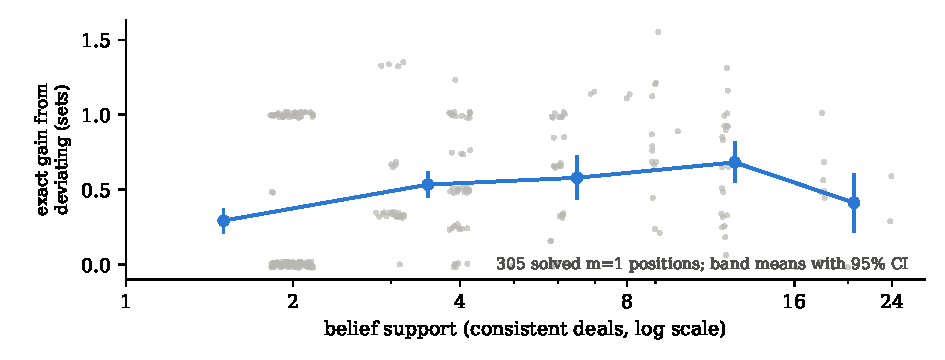
\includegraphics[width=\linewidth]{figs/support.pdf}
\caption{What an exact deviation is worth, against how much the belief leaves
open, over the $305$ solved $m = 1$ positions. Gray points are positions
(jittered for visibility); blue points are means over support bands with 95\%
confidence intervals. The gain rises with support --- and the unsolved
positions lie beyond the right edge of this plot, at a median support of $48$
against a solved median of $3$. That is why the solved-layer means read as
lower bounds, why \S\ref{sec:iibounds} tries to replace that extrapolation
with bounds, and why the honest answer is that the plot cannot be read past
its own right edge.}
\label{fig:support}
\end{figure}

The positions the solver cannot reach are precisely the wide ones --- $16$
unsolved at $m = 1$ with median support $48$, against a solved median of
$3$; $204$ unsolved at $m = 2$ with median support $60$ against a
solved median of $4$. The obvious reading is that both reported means are
therefore \emph{lower} bounds on the gain over the whole layer.

That reading is an extrapolation, and \S\ref{sec:iibounds} tries to replace it
with bounds that hold on every position rather than a slope read past its data.
The attempt does not settle it: the bounds are real, they were validated on
$716$ positions, and they are too loose to decide. It does establish something
smaller and firmer --- that the cheap proxy which \emph{looked} like it settled
the question cannot, because the proxy loosens as the belief widens. No
corrected figure is offered. The honest position is that the direction of this
bias is unknown, not that it is known and favourable.

\subsection{Bounding the layer instead of solving it}
\label{sec:iibounds}

Two thirds of $m = 2$ is unsolved, and the previous section leant on a slope
fitted below the cap to say which way that biases the headline. A slope
fitted over supports $2$--$24$ and read across a gap running to $60{,}480$
deals is an argument, not a measurement. Two quantities replace it, and both
hold by construction on \emph{every} position, reachable or not.

\paragraph{The two bounds.} For a position with belief support $\{d\}$,
weights $\{w_d\}$ and champion value $C$:

\begin{itemize}
\item \textbf{Upper.} $U = \sum_d w_d\,V_{\mathrm{PI}}(d)$, where
  $V_{\mathrm{PI}}(d)$ is the solver run on the single deal $d$. Solving one
  deal is the perfect-information relaxation --- the deviator is told the deal
  and may answer differently in each --- and any genuine
  imperfect-information policy is one the relaxation may also play. Hence
  $V_{\mathrm{II}} \le U$. No new solver is involved: \texttt{ExactII} on a
  single state \emph{is} $V_{\mathrm{PI}}(d)$.
\item \textbf{Lower.} $L = \max_a \sum_d w_d\,\mathrm{champion}(d \mid a)$
  over root actions legal in every deal: play $a$, then revert to champion
  play. One policy is attainable, so $V_{\mathrm{II}} \ge L$. The champion's
  own root action is a candidate, so $L \ge C$ and the bounded gain can never
  come out negative.
\end{itemize}

\paragraph{The control.} Positions with support at most $12$ are also solved
exactly, in the same run and on the same state object, and the exact gain must
lie inside its own bounds. It does, on \textbf{$100/100$}. The control is
computed in place rather than joined to the results of \S\ref{sec:iim2}: that
file keys its rows by game alone, several to a game and only for the positions
it attempted, so any alignment would have been a guess --- and a control built
on a guessed join checks nothing.

\paragraph{The pre-registered answer is: not settled.} Over $248$ positions in
$59$ games, the ones not solved exactly are bounded into
$[\mathbf{+0.2976}, \mathbf{+1.7455}]$. The study's solved mean over the same
games is $+0.3214$, which the interval straddles. The bounds are real and they
are too loose to decide; \path{prereg/ii_bounds.md} fixed that reading
before the run.

\paragraph{Perfect information is a bad bound for this game.} That is the
first thing the run establishes, and it is worth stating because the PI
relaxation is the standard tool reached for here. Where the truth is known it
overshoots by $+0.3278$, against the one-ply policy's $+0.0585$ undershoot ---
five times looser, on the same positions. On $36$ of $248$ positions
\emph{every} deal exceeded its budget and fell back to the trivial figure, so
those are bounded by arithmetic rather than by any search. Above support
$150$, $82\%$ of all deals fall back.

\paragraph{Exploiting the champion at $m = 2$ is almost always one move.}
On \textbf{$88$ of the $100$} positions solved exactly, playing the single best
deviation and then reverting to champion play attains the exact optimum. Over
all hundred the gap averages $+0.0585$ ($95\%$ CI $[+0.0197, +0.0974]$). The
exploitation is a local error and not a sustained plan --- which is what makes
the cheap bound as tight as it is, and is a fact about the champion worth
having on its own.

\paragraph{The same bounds at $m = 1$.} Correcting one layer and leaving the
other resting on the slope would leave a reader unable to tell whether $m = 1$
was checked and held or simply not checked, so it was checked. Over $200$
games the layer has $644$ positions, of which $340$ are pinned --- the belief
admits one deal, the gain is zero by construction, and they are counted
separately rather than averaged in. Of the $304$ with a real belief, $276$ are
solved exactly here, at a mean gain of $+0.4116$ against the $+0.4405$ of
\S\ref{sec:ii} over its $305$; the difference is which positions each run
reached, not a disagreement. The control holds on \textbf{$616/616$}, which
with the $m = 2$ layer's $100/100$ is $716$ positions whose exact value lies
inside its own bounds. One deviation attains the optimum on $543$ of the $616$
--- $88\%$, the same fraction as at $m = 2$, on six times the sample.

Only $13$ of the $304$ sit above the support cap, so at $m = 1$ there is very
little to extrapolate across in the first place: $95\%$ coverage means the
question the previous section worries about is nearly moot here. It is the
long solvable range, not the unsolved tail, that makes this layer useful --- it
is what allows the next paragraph to be measured at all.

\paragraph{The cheap instrument loosens as the belief widens, which is why it
cannot settle this.} Because the one-ply gain is computable everywhere and the
exact gain is not, it looked like the only \emph{matched} instrument spanning
the support cap. Whether it is depends entirely on whether its looseness is
constant in support, and at $m = 2$ that could not be checked: exact values
exist only up to support $12$ there, over which the gap shows no trend
($t = -0.04$). Running the same bounds on the $m = 1$ layer --- cheaper, and
solvable exactly out to support $24$ --- gives the range to check it, and the
answer is that the gap \textbf{grows}:

\begin{center}
\begin{tabular}{lrr}
\toprule
$m = 1$ support & exact minus one-ply & $n$ \\
\midrule
$2$--$4$   & $+0.0785$ & $209$ \\
$5$--$8$   & $+0.2496$ & $31$ \\
$9$--$16$  & $+0.3920$ & $29$ \\
$17$--$24$ & $+0.1667$ & $7$ \\
\bottomrule
\end{tabular}
\end{center}

Slope $+0.0236$ per deal, $t = \mathbf{+6.27}$ over $276$ positions. So a
one-ply figure that flattens or falls above the cap is exactly what a
loosening instrument produces, whether the true gain is flat or rising. The
$m = 2$ null is not evidence that the trend stops; it is evidence that this
instrument stops tracking. Reported here as a measurement of the instrument.

For completeness, what the comparison showed before that was known --- and
which nothing above licenses reading as a fact about Fish. Splitting at the
study's $24$:

\begin{table}[t]
\centering
\begin{tabular}{lrr}
\toprule
support & one-ply gain & $n$ \\
\midrule
$1$--$2$      & $+0.1111$ & $54$ \\
$3$--$8$      & $+0.2618$ & $63$ \\
$9$--$24$     & $+0.3933$ & $52$ \\
$25$--$60$    & $+0.3408$ & $33$ \\
$61$--$150$   & $+0.1155$ & $19$ \\
$151$ and up  & $+0.1899$ & $27$ \\
\bottomrule
\end{tabular}
\caption{One-ply gain against belief support at $m = 1$, split at the study's $24$. Reported for completeness and \emph{not} as a fact about Fish: \S\ref{sec:noneq} shows the cheap instrument's looseness grows with support ($t = +6.27$), so the fall-off in the last two rows is the instrument losing its grip rather than the game getting easier.}
\label{tab:support}
\end{table}

At or below the cap it averages $+0.2541$ ($n = 169$); above it, $+0.2350$
($n = 79$); Welch $t = -0.42$. Taken at face value that says the rise stops.
Taken with the calibration above, it says the instrument stops --- and the two
readings cannot be told apart from this data.

The comparison was \textbf{exploratory} from the start, and the
pre-registration records it as such: it was added after the upper bound turned
out not to bind, and its bands were chosen after seeing the support
distribution. It is left in because the negative result about the instrument is
worth having, and because a comparison that was run and then quietly dropped
once it stopped supporting a conclusion is the thing this project is trying not
to do. The pre-registered verdict is unchanged and stands alone: not settled.

\subsection{Where the disagreements are, and one that is provable}
\label{sec:iidiff}

Comparing the champion's move to the exact optimum's at each hidden decision,
$78$ of $263$ agree ($10$ more exceeded the $300{,}000$-node budget and are
unsolved, not counted either way). Of the $185$ disagreements, $78$ cost
\emph{exactly} zero --- ties broken differently, not errors --- and the rest cost
$+0.5609$ on average, or $+0.2005$ spread over every hidden decision. Their shape does not implicate one component: of $93$ costly
ask-versus-ask disagreements, $47$ share the target only, $11$ the card only,
and $35$ neither. No repair is proposed from that.

Thirteen could not be priced at all, because the declared split was in no
candidate the solver enumerates --- and that set contains every assignment true
in at least one consistent deal. Those claims were true in \emph{no} deal the
record allows. Checked directly, and the weak version of the check refuted the
reading it was built to confirm: testing each card's own holder mask gives
$0/1080$. A declaration can satisfy every card's mask separately and match no
complete deal, because the hand \emph{counts} do not add up --- the failure
\texttt{claim4} names as ``per-card modes can be jointly impossible''.

\begin{center}
\begin{tabular}{lrr}
\toprule
& claims & jointly impossible \\
\midrule
$m = 1$ & $60$ & $\mathbf{7\ (11.7\%)}$ \\
$m = 2 \dots 9$ & $480$ & $0$ \\
\bottomrule
\end{tabular}
\end{center}

Only at $m = 1$, and structurally: there the hand counts are tight enough that
a mis-split is detectably infeasible, while above it there is slack enough that
almost any team-only declaration fits some deal. Every such declaration was
wrong by construction: $+0.000$ sets each against $+0.968$ for the rest,
under the void-era rule these games were played with --- under the award
baseline each would have scored $-1$, a fact the adoption verdict below now
carries.

\subsection{The repair, and why it is not adopted}

A max-flow feasibility test over the live cards decides the question exactly at
any layer, and agrees $40/40$ with brute-force enumeration where enumeration is
available. Supplying the most likely \emph{feasible} declaration instead ---
filtering alone changes nothing, because \texttt{forced\_claim} rebuilds a
declaration from the masks when no candidate survives --- gives, over $6000$
pre-registered pairs:
\[
+0.028,\quad 95\%\ \text{CI}\ [+0.024,\, +0.033].
\]
Every block positive, every block excluding zero, and $27$ wins against $973$
ties and $0$ losses in a representative block: the arm alters play about $0.09$
times a game, so most deals are bit-identical and repairing a claim that could
not have won cannot cost anything.

The bar fixed before the arm existed was $+0.05$. \textbf{It is not adopted},
and the champion is unchanged. A provable error, a free repair, and an effect
smaller than the smallest one this project agreed in advance to care about ---
all three are the finding. One caveat now attaches: the $+0.028$ was earned
under the void rule, where a repaired impossible declaration saved one point
of differential; under the award baseline it saves two, so the arm's value
plausibly doubles and clears the bar. Re-running this 6000-pair design under
the award rule is the one adoption decision the rule correction can
plausibly reverse, and it is queued rather than presumed.

% =====================================================================
% =====================================================================
\section{The all-champion profile is not an equilibrium}
\label{sec:noneq}

Computed with the corrected solver, and therefore not covered by the
withdrawal in Section~\ref{sec:ii}.

Section~\ref{sec:ii}'s figures average over \emph{positions}, and a game can
contain several $m = 1$ decisions. That is the right unit for asking how well
the champion plays the endgame and the wrong one for asking how exploitable it
is: summing gains across positions in one game double-counts a continuation the
deviator only gets to play once. So this takes exactly one position per game ---
the first $m = 1$ decision with genuinely hidden cards --- and lets the deviator
play champion-identically before it and optimally from it.

The value is already a team differential: $+1$ for a half-suit the deviator's
team takes and $-1$ for one the opponents take, so a half-suit changing hands
moves it by $2$, exactly as it moves the set differential
\path{scripts4/exploitability.py} reports. Over 60 games:

\begin{center}
\begin{tabular}{lrr}
\toprule
 & per game & 95\% CI \\
\midrule
sampled rollout best response, whole game & $-0.4875$ & $[-1.2442, +0.2692]$ \\
exact, \textbf{one} endgame decision only & $\mathbf{+0.1111}$ & $[+0.0460, +0.1761]$ \\
\bottomrule
\end{tabular}
\end{center}

The interval excludes zero, so a single seat deviating at a single endgame
decision takes a positive amount --- and if the all-champion profile were an
equilibrium, no single seat could gain by deviating at all. The rollout
responder, deviating for a \emph{whole} game, measured $-0.4875$: it does not
merely fail to find an exploit, it loses ground, which is what
\path{fish4/bestresponse.py} warns strategy fusion can do to a PIMC
responder.

\paragraph{Why the per-game figure is the smaller one, and why it is the right
one.} Of the 60 games, only 22 contain a first $m = 1$ decision with
anything hidden. In the other 36 the belief has \emph{pinned every card} by
the time the endgame arrives --- not a wide support, not a missing position:
all 36 are pinned --- so the closed form already answers them and the
restricted deviator gains exactly zero. Conditional on a hidden decision
existing the gain is $+0.2928$; per game it is $+0.1111$. Quoting the conditional
figure beside a whole-game bound would compare a mean over a favourable subset
against a mean over everything. The 2 games whose first hidden decision
exceeded the node budget are excluded from the denominator rather than scored
zero: unsolved is not worth nothing.

That split is the better description of the champion. Its inference finishes
the endgame outright in 60\% of games; where it does not, it leaves about a
third of a set on the table.

\paragraph{What this does not bound.} The opponents are a \emph{deterministic
realisation} of the champion, seeded from a hash of the observation, and
best-responding to a realisation one can predict is easier than beating the
mixture it came from. The champion mixes at most of these decisions --- over
$41$ hidden $m = 1$ information sets at $12$ seeds each it repeats its move
every time in only $32\%$ of them. So this bounds the realisation, not the
champion as it plays, and the claim is correspondingly narrow: \emph{that}
profile is not an equilibrium.

% =====================================================================
\section{Playing the endgame from the solution}
\label{sec:exactplay}

Section~\ref{sec:iidiff} measures that the champion picks the exact optimum at
under a third of hidden $m = 1$ decisions. \path{fish4/endgame_ii.py} puts
the solver in the agent at exactly those decisions. Duplicate-deal paired
against the identical configuration with the flag off, so everything but the
policy cancels:

\begin{center}
\begin{tabular}{lrr}
\toprule
seed block & set differential & 95\% CI \\
\midrule
$0$ (screen) & $+0.0875$ & $[+0.0307, +0.1443]$ \\
$1$ & $+0.0650$ & $[+0.0033, +0.1267]$ \\
$2$ & $+0.0750$ & $[+0.0150, +0.1350]$ \\
\midrule
pooled, $1200$ pairs & $\mathbf{+0.0765}$ & $\mathbf{[+0.0422, +0.1108]}$ \\
\bottomrule
\end{tabular}
\end{center}

Cochran's $Q = 0.280$ on $2$ degrees of freedom: the three blocks are as
consistent as independent estimates of one quantity get. That matters here more
than the interval does. This project has already had a cell clear the same bar
at $+0.490$, return $+0.068$ on one fresh block and $-0.066$ on a second, and
turn out to be noise; the replications are what separate this from that.

\paragraph{The firing rate is part of the result.} The first version of this
measurement returned $+0.000 \pm 0.000$ over $40$ paired deals in a
single-seat arm, which reads exactly like a clean null and was nothing of the
kind --- the policy had fired \emph{twice}. Raising the caps from $12$ deals
and $50{,}000$ nodes to the study's $24$ and $300{,}000$ changed that count from
$2$ to $2$. A seat faces about $0.075$ solvable hidden $m = 1$ decisions per
game, not because the search is too small but because the champion's belief has
usually pinned the endgame before it arrives --- the same fact
Section~\ref{sec:noneq} reports from the other side, where $36$ of $60$ games
have no hidden first endgame decision at all. Every arm now reports how many
decisions the flagged seats faced and how many the solver answered, and a run
where it never fires refuses to print a differential.

\paragraph{One mechanism, visible in the raw counts.} Over the $1200$
void-era games the policy produced $446$ misdeclarations against the
control's $473$ --- a misdeclaration being a declaration with the right team
and the wrong split, voided in these games, awarded to the opponents under
the current baseline. The solver enumerates only declarations true in some
consistent deal, and each avoided misdeclaration is worth twice as much
under the award rule as it was here (design R4 of the rule-correction
pre-registration re-prices this stack).

\paragraph{Cross-play: the gain is not exploitation of one opponent.} The
obvious objection is that \path{fish4/exact_ii} best-responds to the v0.4
champion, so a gain against that champion might be exploitation of it rather
than better endgame play. Against \texttt{V03\_CHAMPION} --- a different agent,
which the solver's opponent model is simply \emph{wrong} about --- over
1200 paired deals in three disjoint seed
blocks, pooled the same way:
\[
  +0.0637 \quad 95\%\text{ CI } [+0.0306, +0.0968], \quad Q = 0.729 \text{ on } 2 \text{ df}
\]
against $+0.0765$ for the champion it was built to answer. The first
cross-play block alone cleared zero only barely, at
$+0.0750$, $[+0.0100, +0.1400]$, and was used here to weaken a caveat before it
had met the bar the champion arm was held to; it has met it now. The same gain
against an opponent it was not modelling is what one would expect of a policy
that plays the endgame better, and not what one would expect of an exploit. The
null count moves the same way here too: 407 against 443.

The \emph{all} arm cannot settle this and is reported for completeness only:
with every seat flagged both teams are identical, so its differential is about
zero by construction, and $-0.050 \pm 0.198$ over $40$ pairs is what that looks
like.

\paragraph{Not promoted, and why.} The flag is off, and after the cross-play
result only one of the two original reasons still stands.

The first was that a best response is not an equilibrium strategy, so this
might measure only that the policy beats \emph{this} champion.
Section~\ref{sec:noneq} remains a standing reminder that strength against a
named opponent and unexploitability come apart --- but the cross-play row is
direct evidence against that reading here, and the objection is much weaker
than when it was written.

The second stands unchanged: turning the flag on would change the champion, and
the champion is what \path{fish4/exact_ii} models. Every exact figure in
Sections~\ref{sec:ii} and~\ref{sec:noneq} is a statement about the current
champion, and promoting this would invalidate all of them at once. That is a
decision with a cascade behind it, to be taken deliberately and re-measured
afterwards, not a consequence of a good table.

\section{The solver as a critic: a defect found, fixed and shipped}
\label{sec:critic}

\begin{quote}
\emph{Every improvement in this project until now came from a duel. This one
came from a proof, and the duel only confirmed it.}
\end{quote}

The exact solver was built to measure exploitability. It also does something a
duel cannot: it says \emph{which move} was wrong, in a position, with a number
attached. \S\ref{sec:iibounds} established that beating the champion in the
endgame is almost always \emph{one} move --- on $88$ of $100$ exactly solved
$m = 2$ positions and $543$ of $616$ at $m = 1$, a single deviation followed by
ordinary champion play attains the exact optimum. A defect that is one move
wide is a defect that can be looked at.

\paragraph{The move is an ask, and it is riskier than the champion's.} The
improving move is an ask rather than a claim on $131$ of $154$ improvable
$m = 1$ positions and $128$ of $138$ at $m = 2$, so the defect is in ask
selection. Paired within each position --- same belief, same hand, so nothing
about the position can explain the difference:

\begin{center}
\begin{tabular}{lrrrr}
\toprule
& champion's ask & better ask & paired $t$ & $n$ \\
\midrule
$m = 1$ & $p = 0.799$ & $p = 0.218$ & $-18.88$ & $122$ \\
$m = 2$ & $p = 0.611$ & $p = 0.219$ & $-10.02$ & $91$ \\
\bottomrule
\end{tabular}
\end{center}

The better ask is riskier on $113$ of $122$ at $m = 1$ and safer on
\emph{none}. On $73$ of those $122$ the champion asked a card it was
\textbf{certain} to get, and that was still a mistake.

\paragraph{But it is certainty, not probability.} The obvious fix --- weigh
the success probability less --- does not work, and the data says so before any
duel. The objective is $\mathrm{score}(a) = p(a) + F(a)\cdot w$, and since the
argmax is scale-invariant, $p + F\cdot(kw)$ ranks asks exactly as
$(1/k)p + F\cdot w$: the existing objective already spans every positive weight
on $p$. Searching that one-parameter family over $388$ endgame positions
carrying the exact one-ply value of every candidate ask returns $k = 1$. No
change.

What helps is the information term, which rewards asks the belief cannot call.
Held out by \emph{game}, so positions from one deal cannot sit on both sides:

\begin{center}
\begin{tabular}{lrr}
\toprule
model & train & held out \\
\midrule
champion (0 parameters)      & $+0.0805$ & $+0.1498$ \\
scale $k$ (1 parameter)      & $+0.0805$ & $+0.1498$ \\
$\mathtt{info} = +2.00$      & $+0.1236$ & $+0.1591$ \\
$\mathtt{certain} = -0.50$   & $+0.1212$ & $+0.1784$ \\
full search (11 parameters)  & $+0.1786$ & $[+0.1281, +0.1884]$ \\
\bottomrule
\end{tabular}
\end{center}

The eleven-parameter fit gains most on train and its held-out score is an
\emph{interval}, not a number: run at four search seeds with the budget fixed,
it lands anywhere from below the champion to above every one-parameter model.
That is a property of which random restarts came up, not of the model, and one
run of it would have reported whichever number that happened to be. The
one-parameter models have no such freedom --- their grid is exhaustive --- which
is a reason to prefer them beyond their score. $\mathtt{info} = +2.0$ was
chosen on train and confirmed by leave-one-game-out cross-validation inside the
training games; $\mathtt{certain}$ scored better on the held-out set and was
\emph{not} chosen, because picking it would be picking by the check.

\paragraph{Three duels, because an effect measured against a weak base does not
transfer by assumption.} The correction applies only when at most two
half-suits are live. Every run was pre-registered with its arm, size, seeds and
readings fixed first, and on deals the fit never saw:

\begin{center}
\begin{tabular}{lrrr}
\toprule
& diff (sets) & $95\%$ CI & pairs \\
\midrule
vs champion, registered   & $+0.0835$ & $[+0.0338, +0.1332]$ & $2000$ \\
vs champion, replication  & $+0.0980$ & $[+0.0480, +0.1480]$ & $2000$ \\
vs champion, pooled       & $+0.0907$ & $[+0.0555, +0.1260]$ & $4000$ \\
\textbf{on top of what ships} & $\mathbf{+0.1220}$ &
  $\mathbf{[+0.0711, +0.1729]}$ & $2000$ \\
\bottomrule
\end{tabular}
\end{center}

The last row is the one that moved a default and the one to quote: the site
plays a depth-3 belief-space lookahead, which searches exactly the positions
this correction is about, and it might already have been finding these asks.
It was not --- the effect is if anything \emph{larger} on the stronger base,
$15$ of $16$ blocks positive.

\paragraph{What was predicted and was wrong.} The pre-registration said the
effect would be small and the test might be underpowered to see it: the
correction moves a handful of decisions a game, and offline it was worth
$+0.0093$ in half-suit units. It is worth $+0.1220$ sets in play, about what
running the entire exact solver in the endgame gains ($+0.0765$). The
prediction that the endgame is too thin a slice of the game to matter was
wrong, and it is recorded here because it was written down first.

\paragraph{It wins more; it is not harder to exploit.} Winning duels and being
less exploitable are different claims, and the solver can be asked the second
one directly: it takes the opponents' policy as an argument, so the same
positions can be solved twice. Over $285$ $m = 1$ positions from champion
self-play, each solved against the champion and against the champion plus the
correction --- same position, same belief, same hand, so nothing about the
position can explain a difference:

\begin{center}
\begin{tabular}{lrr}
\toprule
paired change & estimate & $95\%$ CI \\
\midrule
the policy's own value & $+0.0189$ & $[-0.0132, +0.0509]$ \\
what a best response takes & $-0.0002$ & $[-0.0264, +0.0260]$ \\
the gap between them & $-0.0190$ & $[-0.0587, +0.0206]$ \\
\bottomrule
\end{tabular}
\end{center}

Neither clears zero, and the two nulls are not the same null. The own-value
change is simply underpowered --- a half-width of $0.032$ around $+0.019$, with
the sign the in-play result predicts. The best-response change is
\emph{pinned}: $-0.0002$ with a half-width of $0.026$, an interval that
excludes any reduction the size of the $+0.1220$ the correction gains in play.
A best response still takes the same amount.

So the correction does not buy its winnings by closing the hole. That is a
limit on the method rather than on this particular fix, and it is worth stating
because the method is the interesting part of this section: an exact best
responder used as a \emph{critic} improves average-case play, and nothing about
fixing the moves it flags makes the worst case harder to reach. Exploitability
and strength are being measured, and they moved independently.

\paragraph{Pushing the correction up the game measured deception, not strength.}
What happened when the correction was extended past the endgame is reported in
full because it is the sharpest methodological result in this paper, and
because half of it is a finding about the game.

The correction applies below a threshold $m$ of live half-suits. A
pre-registered ladder raised the threshold one rung at a time, each rung
duelling the incumbent, each shipping only on a CI clear of zero. Every rung
cleared, and the rungs \emph{grew}: $+0.1220$ to $m \le 2$, $+0.3025$ to
$m \le 3$, $+0.6995$ to $m \le 4$, $+1.0125$ to $m \le 5$, and $+4.2790$ for
the amended coarse step to always-on --- a bigger single gain than the whole
v0.3-to-v0.4 release. Eight of eight blocks positive at every rung, no
timeouts, engine digests matched.

All of it was an artefact of \emph{who was on the other side of the table}.
Each rung duelled the sibling configuration, and the sibling's opponent model
conditions on which half-suit a player chooses to ask. Information-seeking
asks violate that model systematically, so they poison the sibling's
inference; the rungs grew with $m$ because a higher threshold spends more of
the game poisoning. Against the v0.3 champion --- a foreign opponent whose
inference is built differently --- with every configuration playing the same
$500$ deals and per-deal differencing against no correction:

\begin{center}
\begin{tabular}{lrr}
\toprule
threshold & margin over v0.3 & paired $\Delta$ vs.\ no correction \\
\midrule
none      & $+3.006$ & --- \\
$m \le 2$ & $+2.914$ & $-0.092\ [-0.448, +0.264]$ \\
$m \le 3$ & $+2.568$ & $-0.438\ [-0.829, -0.047]$ \\
$m \le 5$ & $+1.526$ & $-1.480\ [-1.888, -1.072]$ \\
always on & $-2.160$ & $-5.166\ [-5.643, -4.689]$ \\
\bottomrule
\end{tabular}
\end{center}

\begin{figure}[t]
\centering
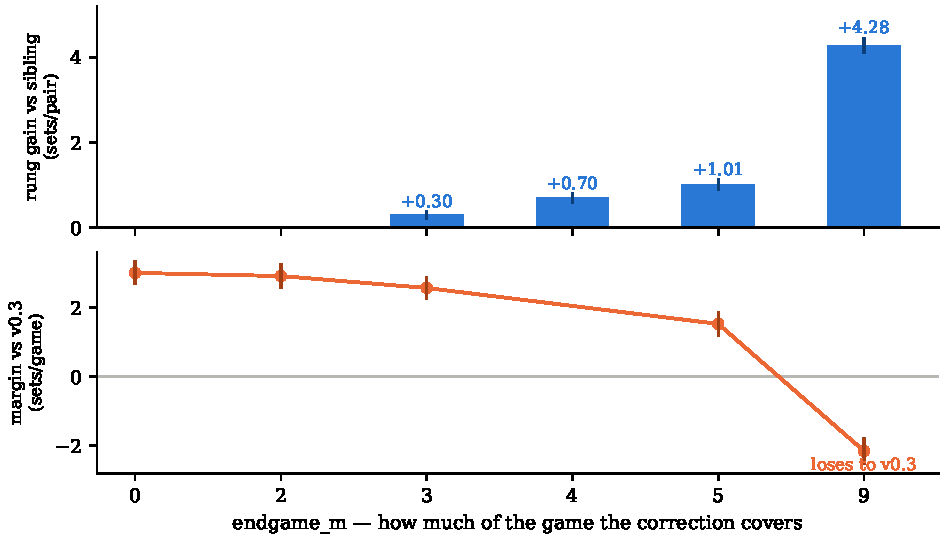
\includegraphics[width=\linewidth]{figs/ladder.pdf}
\caption{The deception ladder, both measurements of the same knob. Top: each
pre-registered rung's gain over its sibling incumbent, growing with the
threshold $m$ --- eight of eight blocks positive at every rung. Bottom: the
same configurations against the foreign v0.3 champion on $500$ shared deals;
every rung above the shipped $m \le 2$ is a significant loss, and always-on
loses to v0.3 outright. The panels share an x-axis, so each column is one
configuration read against two opponents: the rungs were not measuring
strength, they were measuring how much of the game was spent poisoning the
sibling's opponent model.}
\label{fig:ladder}
\end{figure}

Monotone, and the mirror image of the sibling ladder
(Figure~\ref{fig:ladder}): every rung above $2$ is
a significant \emph{loss} against a foreign opponent, ending at a
configuration that loses to v0.3 outright. The always-on rung was shipped for
minutes on the strength of $+4.28$ and reverted when the first cross-play
block came back; every rung above $2$ is withdrawn, and the shipped threshold
is back at $m \le 2$ --- whose foreign-relative effect is a paired tie, and
which alone rests on evidence that is not a sibling duel.

Three readings, stated separately. \emph{About the game}: exploiting an
opponent model that conditions on action choices is worth several sets per
game in six-player Literature, which makes deception a first-class strategic
resource here, found by accident and measured to $\pm 0.24$. \emph{About the
method}: a pre-registered ladder with a fixed stopping rule, eight-of-eight
block agreement, matched engine digests and growing effects passed every
check this paper uses --- and measured the wrong quantity at every rung,
because no rule asked \emph{against whom} the gain was defined. Robustness
of the opponent pool now belongs beside pre-registration in the discipline,
not downstream of it. \emph{About the correction}: the $+0.1220$ of the
preceding paragraphs is a gain against the engine's own family, bounded
against v0.3 inside $[-0.448, +0.264]$; the exact solver's diagnosis stands,
and what its repair bought is play that is better against the family and no
worse outside it.

\paragraph{The same question against an engine nobody here wrote.} Everything
above still measures the correction against relatives: the sibling ladder, and
a v0.3 that shares this project's rules engine and most of its ancestry. What
the withdrawal actually demands is an opponent with \emph{no} shared code, and
one exists: \textbf{FishBot v0.7} by dylann4500, an independently written
C++ engine for the same six-player, 54-card game --- different author,
different belief representation, different search, its 55-parameter policy
frozen upstream after self-play tuning. It plays under this engine's arbiter
through a process bridge that replays the public history to the frozen policy and
legality-checks every move it proposes, substitutions counted rather than
hidden; zero were needed across the $2{,}000$ games this section reports.
Two caveats travel with the comparison: v0.7 was tuned for a rule variant
with out-of-turn declarations and plays here under this paper's rules, which
its policy is told; and it is one foreign opponent, not a population. A
third caveat --- that the first run scored misdeclarations under this
engine's void-era rule while v0.7's native game awards them --- was removed
by re-running the whole design under the award baseline, below.

The check was pre-registered before the first scored game
(\path{prereg/foreign_opponent_m2.md}), outcomes fixed in advance: the
deployed configuration with the correction on, and the same configuration
with it off, each played three copies of v0.7 on $250$ deals in both
rotations --- $500$ games per arm --- the statistic being the on-minus-off
difference of set margins on the same deal and rotation. The registered
question was reversal, and the answer is no: $-0.0300$
$[-0.1081, +0.0481]$ against Dylan's v0.7, at a power sized for
deception-scale flips. The sharper reading is what the interval
\emph{excludes}: $+0.1220$, the correction's own sibling-measured size. On a
third, unrelated opponent the effect is a tie, so the sibling number does not
transfer at anything like face value --- the section's finding again,
demonstrated this time on an engine from outside the project entirely, and
converging with the upstream author's own documentation, which reports of its
final tuning stage that ``the advantage is a self-play advantage \dots\ it
does not transfer.''

The context the check ran in: with the correction on, the deployed
configuration beats v0.7 by $+2.448$ sets per game ($+2.478$ with it off),
taking 64.3\% of decided sets across the $1{,}000$ games. That margin is a
statement about this game under this paper's rules against an engine tuned
under slightly different ones, and it is quoted as context, not as a ranking
of the two projects; the measurement the design paid for is the paired
difference, which needs no ranking to be valid.

\paragraph{The same check, rule-matched.} When the misdeclaration baseline
flipped (\S\ref{sec:game}), the design was re-registered and re-run from
scratch under the award rule (design R2 of
\path{prereg/rules_award_baseline.md}: fresh seeds, its own journal, the
rule pinned in the runner rather than inherited), which makes the two
engines agree on what every wrong declaration costs --- v0.7's native risk
model is now exactly the rule in force. Over another $500$ paired games the
answer does not move: $-0.0440$ $[-0.1344, +0.0464]$ against Dylan's v0.7
under the award rule --- no reversal, and the sibling-measured size is again
excluded. The margin context: $+2.544$ sets per game with the correction on,
$+2.588$ with it off, 64.3\% of decided sets over the $1{,}000$ games ---
the share to the decimal of the void-era run, on disjoint deals, under a
different scoring rule.

What the rule-matched run adds is the accounting of the rule itself: $466$
sets in those $1{,}000$ games were misdeclarations --- wholly-held
half-suits declared with the wrong split, each now a set for the other side
--- and they divide $160$ against this engine to $\mathbf{306}$ against
v0.7. The correction the void rule had been silently granting was worth
nearly twice as much to the opponent, so scoring misdeclarations properly
\emph{widened} nothing --- it is the reason the margin held rather than
shrank when the game switched to the rule v0.7 was built for. This paper
first attributed that gap to v0.7's forced declarations, which come from a
sampled best guess where this engine declares the exact posterior MAP
(\S\ref{sec:claiming}). The next paragraph withdraws that attribution: the
split is unchanged by a repair that fixes the forced declarations outright,
so it belongs to their voluntary declaration gate instead.

\paragraph{A defect in the bridge, found from the other side, that had been
flattering this engine.} Every figure above was taken through this project's
bridge into v0.7, and an adversarial read of their C++ --- their source, not
their paper --- found a defect in that bridge rather than in either engine.
Forced to declare, their own driver picks the first live half-suit the mover
\emph{holds a card in} (\texttt{engine/src/game.hpp:535}); this bridge passed
the first live half-suit, full stop. Their \texttt{bestGuess} was therefore
periodically asked to name all six owners of a half-suit it held nothing of
--- a question with no anchor in its own hand, which their own driver never
puts them in a position to be asked, and which under the award rule hands
the set here.

The defect ran in this engine's favour, which is the direction a project does
not catch by reading its own results and nodding. Priced paired --- all
$10{,}000$ deals replayed under both bridge revisions, identical deals and
identical seating, the same duplicate-deal design every screen in this paper
uses (\path{scripts4/bridge_bug_price.py}) --- it is worth $\mathbf{-0.0784}$
$[-0.0881, -0.0687]$ sets per game: real, and about $3\%$ of the margin. It
is also an order of magnitude smaller than the $0.30$ sets per game the same
read estimated from $40$ games, which is what the paired instrument is for.
Under the repair their declaration accuracy rises from $76.18\%$ to
$78.87\%$, while this engine's moves from $96.65\%$ to $96.49\%$ --- the
control that confirms the repair touches only their side of the bridge.

What the repair does \emph{not} move is the misdeclaration split, and the
reason corrects the mechanism the previous paragraph had assumed. The
anchorless forced declarations were \emph{ownership}-class errors ---
half-suits the opposing team still held a card of --- whereas the
$160$-to-$306$ split counts \emph{allocation}-class errors, wholly-held
half-suits declared with the wrong split. Across the same $10{,}000$ paired
deals the allocation split is flat: $2{,}784$ against v0.7 before the
repair, $2{,}775$ after. The finding that this engine misdeclares roughly
half as often survives intact; the explanation for it does not, and the gap
is a property of their voluntary declaration gate rather than of a question
this bridge was mis-posing. The pre-registered R2 contrast is likewise
undisturbed,
because the defect is common-mode across its two arms --- both the
correction-on and correction-off games ran through the same bridge, and a
paired difference cannot see an error that appears identically in both
halves of the pair. What is restated is the \emph{context} the R2 file
reports beside its verdict: the margin and set share, which are absolute
rather than paired, and which the corrected head-to-head below supersedes.

\paragraph{The head-to-head, re-measured through the repaired bridge.}
\label{sec:headtohead}
This
is the figure the paper stands behind, and the only one taken through bridge
revision~2: $10{,}000$ games on the same deals the retracted run used, seats
rotated so neither engine opens more often, both engines on their native
misdeclaration rule, zero substituted moves and zero unfinished games
(\path{scripts4/mega_match.py} $\rightarrow$ \path{results/mega_match.json}).
Matching the withdrawn run deal for deal is deliberate: it makes the
replacement a like-for-like correction rather than a differently-powered
second opinion.

\begin{center}
\begin{tabular}{lr}
\toprule
margin & $\mathbf{+2.3466}$ $[+2.2928, +2.4004]$ sets/game \\
sets & $56{,}733$ to $33{,}267$ ($63.04\%$ of decided) \\
games won & $80.41\% \pm 0.78$ ($8{,}041$W / $0$T / $1{,}959$L) \\
ask hit rate & $51.75\%$ against $48.14\%$ \\
declaration accuracy & $\mathbf{96.49\%}$ against $\mathbf{78.87\%}$ \\
\bottomrule
\end{tabular}
\end{center}

\noindent The mechanism of the margin is in the last row and not the one
above it. A $3.6$-point edge in ask accuracy is worth something, but the two
engines find cards at broadly comparable rates; where they diverge is in
knowing when a half-suit is \emph{finished}, and an $18$-point gap there is
the difference between cashing a set and handing it over. That is the same
claim \S\ref{sec:claiming} makes from the inference side, arrived at here
from the scoreboard.

\paragraph{How much of the margin is that, exactly.}
\label{sec:res-headline} The paragraph above is a
qualitative reading of two rows, and it had never been priced. It can be:
every declaration in a game is either right or one of two kinds of wrong, and
under the award rule each wrong one moves the margin by two sets, so the
scoreboard decomposes exactly. Over $600$ cross-engine games
(\path{scripts4/margin_decomposition.py}):

\begin{center}
\small
\begin{tabular}{lrr}
\toprule
component & rate & contribution to margin \\
\midrule
measured margin & --- & $+2.3466$ $[+2.2928, +2.4004]$ \\
their ownership-class errors & $0.5667$/game & $+1.1334$ \\
their allocation-class errors & $0.2775$/game & $+0.5550$ \\
our own wrong declarations & $0.1759$/game & $-0.3518$ \\
\midrule
everything else & --- & $+1.0100$ $[+0.9573, +1.0627]$ \\
\bottomrule
\end{tabular}
\end{center}

\noindent \textbf{Fifty-seven per cent of the margin is declaration
accounting.} The edge is real and it is nearly fivefold --- we declare wrongly
$0.176$ times a game against their $0.844$ --- but it is a \emph{declaration}
edge, and
this project has spent the large majority of its compute on the ask objective.
The residual, everything the asking and the inference and the lookahead
between them produce once the declarations are netted out, is $+1.010$ sets
per game: a real margin, and a little over two fifths of the headline one.

These figures are computed on the same $10{,}000$ games the headline margin
is, which took a correction. They were first taken from a $600$-game probe
and quoted beside a margin from the large block, which invites a reader to
apply a ratio measured on one population to a number measured on another.
The two agree --- the probe put their error rate at $0.918$ a game against
$0.844$ here, and the share at $61\%$ against $57\%$ --- but the version on
the headline's own games is the one to quote.

This is a decomposition of where the sets landed, not a counterfactual. A
declaration that did not happen changes every ply after it, and no arithmetic
on a finished game recovers those plies; the residual row is what remains
after the netting, not the margin a differently-declaring v0.7 would have
conceded. The distinction is worth insisting on because the temptation is to
read the last row as ``our true strength'', and it is not that.

\paragraph{And what the other $39\%$ is made of.} The residual --- everything
asking, inference and search produce once the declarations net out --- has a
shape that follows from the rules. Every set is won by declaring a half-suit
your team holds, so once misdeclarations are accounted for what remains is the
race to \emph{assemble} half-suits, and that race has exactly two factors which
multiply: how many asks a team gets to make, and how many of them land. This
paper has reported the second since v0.4 and has never reported the first.
Over $800$ cross-engine games (\path{scripts4/acquisition.py}):

\begin{center}
\small
\begin{tabular}{lrrr}
\toprule
per game & ours & v0.7 & difference \\
\midrule
turns & $57.250$ & $52.562$ & $\mathbf{+4.688}$ $[+3.962, +5.413]$ \\
asks & $51.894$ & $48.265$ & $+3.629$ $[+3.102, +4.155]$ \\
asks that landed & $26.731$ & $23.066$ & $+3.665$ $[+3.129, +4.201]$ \\
half-suits assembled & $5.008$ & $3.416$ & $+1.591$ $[+1.418, +1.765]$ \\
plies holding a set unspoken & $78.166$ & $32.440$ & $+45.726$ $[+41.5, +49.9]$ \\
\bottomrule
\end{tabular}
\end{center}

\noindent Splitting the $3.665$-card gap at the mean gives $+1.802$ to volume
and $+1.863$ to conversion: \textbf{almost exactly half and half}. We take
$4.7$ more turns a game than v0.7, and that is worth as much as the
$3.7$-point edge in ask accuracy this paper has been quoting as the mechanism.
Tempo is not a term in our objective, is not a knob anywhere in the engine,
and has never appeared in a results table --- it is a by-product of asking
well, and it accounts for half of what asking well is worth.

\paragraph{The last row is the one that costs us.} We hold assembled
half-suits for $78$ plies a game against their $32$, and our own declaration
accuracy falls monotonically with how long we have held the set:

\begin{center}
\small
\begin{tabular}{lrrr}
\toprule
plies held assembled & declarations & wrong & error rate \\
\midrule
$0$ (never owned it) & $6$ & $6$ & $1.000$ \\
$1$--$9$ & $2797$ & $46$ & $0.016$ \\
$10$--$29$ & $517$ & $27$ & $0.052$ \\
$30$--$79$ & $454$ & $23$ & $0.051$ \\
$80+$ & $238$ & $28$ & $\mathbf{0.118}$ \\
\bottomrule
\end{tabular}
\end{center}

\noindent Holding is not the cause and the direction of the arrow matters: a
set you can place, you declare, so ``held long'' and ``could not place'' are
nearly the same event. What the table establishes is that being unable to
place a set is \emph{visible early}. And by \S\ref{sec:claiming}'s channel
argument, early is when it can still be acted on --- once the half-suit is
ours no opponent can ask in it, so nothing they do will place it, and the only
remaining channel costs one of our turns.

There is time. Over the $130$ half-suits we declared wrongly, the median
number of \emph{our own} turns between assembling the set and the deadline is
$25.5$, and only $16$ of $130$ were assembled with no turn left to spend. The
lever is reachable in $88\%$ of the cases that go wrong.

Whether spending those turns pays is a different question and this paper has
already answered a version of it in the negative: \S\ref{sec:perpetual}'s
signalling protocol cut nulls by $20\%$ and returned $+0.002$ $[-0.086,
+0.090]$ sets per pair, and it is switched \emph{off} in the deployed
configuration. What the measurements above add is not a new mechanism but a
different \emph{trigger}: that protocol fires when the current turn is cheap,
and the errors are concentrated in half-suits identifiable a median of $25$
turns before the turn gets cheap. Whether a deadline-priced trigger changes
the answer needs its own pre-registration, and the error-value result of
\S\ref{sec:res-pathledger} says what it will be measured against: one avoided
misdeclaration is worth about $1.8$ sets, and a spent turn has to cost less
than that times the chance the signal actually places the split.

\paragraph{What their errors are made of, which is not what we guessed.} The
obvious hypothesis about the ownership-class leak --- the $0.650$ sets a game
they hand over by declaring a half-suit we still hold a card of --- was that
our \emph{silence} causes it: under the no-bluff rule an ask certifies a
holding, so a half-suit we have never asked in is one their posterior has
little reason to place us in. That is backwards. Over the same games, the $398$
cards of ours sitting inside their $390$ ownership errors split as

\begin{center}
\small
\begin{tabular}{lr}
\toprule
publicly pinned to us by an ask we had won & $0$ \\
never publicly moved since the deal & $398$ \\
\bottomrule
\end{tabular}
\end{center}

\noindent Their engine does not misplace a card it has seen move; it only ever
loses one with no public trace. And the leak concentrates where we have
spoken, not where we have been quiet. Weighting by exposure --- plies during
which our team held exactly one card of a live half-suit --- gives $45.4$
ownership errors per $1{,}000$ plies in half-suits we had asked in against
$0.675$ where we had not, a rate ratio of $67$ $[42, 107]$. Sorted by what had
happened in the half-suit before they declared it, $1{,}927$ declarations
followed both an ask of ours and a later successful ask that took one of that
half-suit off us, and $19.25\%$ of those were ownership-wrong; $411$ followed
only the taking, and $3.16\%$ were.

The mechanism this points at is specific, and it is a hypothesis about their
engine formed from outside it rather than a reading of their source. Our ask
certifies that we hold at least one \emph{other} card of the half-suit. When an
opponent later takes one card of it off us, their inference appears to treat
that certification as discharged --- as though ``at least one'' had been
``exactly one'' --- and every card it then loses is one that never moved in
public. We are not building a feature on this. An exploit of one engine's
inference is exactly the shape of the withdrawn deception ladder of
\S\ref{sec:critic}, and a term that farmed it would grow with its dose against
v0.7 and mean nothing anywhere else. It is reported because a margin whose
majority component has an identified cause is a different object from one whose
does not, and readers of the head-to-head are entitled to know which they have.

\paragraph{What this measurement is, stated with the other project's own
scope in view.} Their paper is unusually careful about what it does not
claim, and the sentence that matters here is theirs: ``Whether FishBot v0.7
is the strongest Canadian Fish agent anyone has built \dots\ the paper does
not establish and does not claim. The comparison class contains only agents
this project wrote.'' Their limitations section names the missing
ingredient exactly --- ``there are no independently authored six-player Fish
agents to compare against, which is why \S1.2 confines the paper's
comparative claim to this project's own lineage'' --- and lists an
independently authored opponent first among the things a comparative claim
beyond that lineage would require \citep{dylan2026fishbot}.

That ingredient now exists in both directions, and it is worth being
precise about what each side may therefore say. We can report a margin
against an engine nobody here wrote, which is a stronger kind of evidence
than either project's internal ladders: $+2.347$ $[+2.293, +2.400]$ sets per
game, $63.0\%$ of decided sets, over $10{,}000$ games under rules both engines
implement natively, with zero substituted moves and a bridge whose one known
defect has been found, priced and repaired. What that does \emph{not} establish
is a global ranking of the two projects, and this paper declines that claim
for the same reasons theirs does: one opponent is not a population, their
engine was frozen before ours had the exhibition bridge to test against,
and neither project has run the other's configuration search against its
own. What the number does establish is narrower and, for both papers,
new: the first six-player Literature result measured across an engine
boundary rather than inside one lineage --- which is precisely the
instrument their limitations section asks for, and the one this paper
spent \S\ref{sec:critic} demonstrating that a project cannot build for
itself.

\paragraph{Under the award rule the correction itself no longer earns its
place, and is withdrawn.} Designs R3 and R4 of the same pre-registration
close the loop. R3, the declaration-threshold sanity: against $0.999$ the
shipped $0.97$ bar produces \emph{bit-identical} games --- $0$ of $200$
pairs diverge, $+0.0000$ exactly --- and against $0.90$ the difference is
$+0.0400$ $[-0.0278, +0.1078]$; the void-era finding that any high bar
plays the same survives the rule change, as its rule-invariant mechanism
said it should. R4, the correction stack re-priced: the registered
expectation was that the sign would hold and the size could move. The
expectation was wrong, and it is reported because it was written first:
under the award rule the deployed configuration WITH the $m \le 2$
correction scores $-0.1040$ $[-0.2184, +0.0104]$ against the same
configuration without it, over $500$ fresh pairs --- and the correction arm
misdeclares \emph{more} ($123$ against $106$, again wholly-held splits; both
arms are counted the same way, so the comparison is what it looks like). The mechanism is not
mysterious: the correction's $d_{\text{info}} = 2.0$ was fitted against
solver targets whose continuations priced a wrong declaration at zero, and
the game no longer plays that price. Taken with the foreign tie above
($-0.0440$ under the matched rule), the correction fails, under the
baseline rule, the CI-excludes-zero bar every shipped knob in this project
is held to. It is withdrawn from the deployed configuration ---
\texttt{V06\_DEPLOYED} in the registry is \texttt{V04\_COMBINED} without it
--- and the exact-solver diagnosis behind it, which is rule-invariant,
awaits a refit against award-rule targets: the solver journals now carry
the rule in their resume fingerprints so that refit cannot silently mix
eras. The void-era $+0.1220$ stands as what it always was, a measurement
of the void-era game.

\paragraph{Their one load-bearing mechanism, ported and measured here: it
does not transfer.} The other project's attribution study credits a single
coordinate with essentially the whole gain of its v0.7 cycle --- a
\emph{contestation} term that scores a candidate ask by
$(1 - p_{\text{hit}}) \times (\text{opponent-held mass of the half-suit}/6)
\times (\text{cards of it nobody can place}/6)$ and carries a strongly
positive weight, deliberately spending likely-miss asks in
opponent-dominated, still-ambiguous half-suits
\citep{dylan2026fishbot}. Because their engine and ours now play the same
game under the same rules, that claim is directly testable outside the
lineage it was measured in, which is the kind of question neither project
could ask alone.

Design R6 of the pre-registration ports it and sweeps the dose in both
directions, with two arms of a second idea alongside --- a
\emph{silence prior} that down-weights sampled worlds in which a live
half-suit already sits wholly within one team, on the ground that a team
holding all six and able to place them would usually have declared. Seven
arms plus an unmodified baseline each played $500$ games against three
copies of v0.7 on identical deals and rotations, paired against the
baseline: $4{,}000$ games, zero substituted moves.

\begin{table}[t]
\centering
\begin{tabular}{lrr}
\toprule
arm & paired $\Delta$ vs.\ baseline & margin over v0.7 \\
\midrule
baseline (neither knob)          & ---                       & $+2.732$ \\
contestation $-1.0$              & $-0.4200\ [-0.7137, -0.1263]$ & $+2.312$ \\
contestation $-0.3$              & $-0.2400\ [-0.5085, +0.0285]$ & $+2.492$ \\
contestation $+0.3$              & $-0.3200\ [-0.5790, -0.0610]$ & $+2.412$ \\
contestation $+1.0$              & $-0.2920\ [-0.6261, +0.0421]$ & $+2.440$ \\
contestation $+3.0$              & $-1.1240\ [-1.4735, -0.7745]$ & $+1.608$ \\
silence $\delta = 0.7$           & $-0.1960\ [-0.4775, +0.0855]$ & $+2.536$ \\
silence $\delta = 0.9$           & $-0.2880\ [-0.4883, -0.0877]$ & $+2.444$ \\
\bottomrule
\end{tabular}
\caption{Seven arms against three copies of v0.7 on identical deals and rotations, each paired against an unmodified baseline: $4{,}000$ games, zero substituted moves. Every arm loses, and the two largest weights lose most --- a dose-response, which refutes the mechanism rather than merely failing to find it.}
\label{tab:contestation}
\end{table}

Every arm is negative; four are significantly so, and the largest positive
dose is the worst cell in the table. No arm clears the registered bar, so
by the outcome fixed in advance neither knob ships, stages 2 and 3 do not
run, and the negative is reported rather than swept into a footnote. The
strongest reading the data supports is monotone in the wrong direction:
the more of their mechanism we add, the more of our margin over them we
lose.

This is the third time this paper has watched a gain fail to survive a
change of opponent family, and the first time in the direction that costs
\emph{us} something to admit. The deception ladder's rungs were real
against siblings and vanished against v0.3; the endgame correction was
real under one scoring rule and reversed under another; and their
contestation term is, by their own careful measurement, worth several
points inside their engine and is worth nothing but damage inside ours.
The mechanism is not thereby refuted --- it plainly works where it was
fitted --- and the honest conclusion is narrower and more useful than
either ``it works'' or ``it does not'': an ask-scoring coordinate tuned
against one belief representation is not a portable strategic insight,
even between two engines playing an identical game. Their belief is a
Sinkhorn approximation seeded by a behavioural prior; ours is exact
counting reweighted by a choice model. A term that pays in the first is
apparently already priced in the second.

\paragraph{What did not change.} FishBot4's own defaults. The champion is the
reference point for every measurement in this paper, and moving it would
silently reprice all of them at once; the correction remains in the archival
\texttt{V04\_COMBINED} spec exactly as measured (its withdrawal from the
\emph{deployed} configuration under the award rule is the previous
paragraph's, and the registry's, record). A test requires whole games to
be \emph{bit-identical} when the knob is off, and requires the first divergence
to fall at two live half-suits or fewer when it is on --- checked by replaying
the shared prefix, not by asking the agent where it was.

\section{What this says about playing Fish}
\label{sec:strategy}

The results have readings that do not require an engine, and we state them
because a study of a game people play ought to say something to the people
playing it.

\paragraph{Watch where opponents ask, not just what they ask for.} This is the
finding of the paper, and it is actionable at the table. A player who asks in a
half-suit is probably deep in it, in rough proportion to how many of its cards
they hold, and that single inference is worth more than every other improvement
we made combined. Concretely: when an opponent asks in hearts, do not only note
the hard fact that they hold at least one heart --- shift weight toward their
holding several. The engine's version of this is one parameter, and it is worth
about $1.9$ sets per duplicate deal-pair against a strong opponent that ignores
it.

\paragraph{An exact rule for the perfect-information endgame.} Once every
remaining card is public, the game is solved in closed form: the team on move
scores every live half-suit in which it holds at least one card, and the
opponents score the rest. Footholds only shrink and a well-informed asker never
misses. The practical corollary is that in a fully-known endgame the only thing
that matters is \emph{how many live half-suits your team has a foothold in when
it is your turn} --- not how many cards, not which cards.

\paragraph{Do not agonise over when to declare --- but never guess.}
Reproducing v0.3's finding on a much better posterior: raising the
declaration bar from $0.97$ to $0.99$ changes essentially no decisions. The
reason is structural rather than statistical. If your team genuinely holds
all six cards of a half-suit, no opponent holds any card of it, so no
opponent can legally ask in it --- and a declaration by a team that does not
hold all six gives the set to you. Waiting is close to free, and that
mechanism is rule-invariant. What the award rule changes is the price of
impatience: a guessed split that used to void the set now hands it to the
other team, a two-set swing in the differential. Wait until you know the
split; the rule correction doubled the fine for not waiting.

\paragraph{Two tie-breakers really do hold up.} When two asks look about equally
likely to land, prefer the one that, if it misses, hands the turn to the
opponent with fewer cards, and prefer to fight in half-suits your team is
already winning. v0.3 measured that pair at $+1.41$ sets per deal-pair; with an
inference layer good enough to make the primary criterion much sharper, they are
still worth $+1.08$. Better card-reading does not make positional judgement
redundant.

\paragraph{The endgame is bookkeeping, so do the bookkeeping.} Every one of 200
measured games reached a position where no ask anywhere could succeed: the sets
were decided and only the declarations were left. Two consequences for a human.
First, the last few turns are not a contest, so spend your attention earlier.
Second --- and this is the one people get wrong --- if your team holds a half-suit
outright, \emph{no opponent can legally ask in it}, so it cannot be taken from
you by any ask or by any opposing declaration. There is never a reason to
rush that declaration. In our void-era games, half-suits that reached ``ours
but we cannot place the split'' were misdeclared $23.4\%$ of the time
against $0.92\%$ otherwise --- a factor of $25$ --- and under the award rule
each of those is no longer a voided set but a set \emph{donated}. Almost
every one is a self-inflicted wound, and the wound now costs twice as much.

\paragraph{You can talk, and most players do not realise it.} You may not ask
for a card you hold. So asking for a card \emph{proves to the table} that you do
not have it --- and when your team already owns the half-suit, the ask cannot
lose you anything, because no opponent holds a card of it to give. In that
situation an ask is a free, legal message to your partners telling them exactly
where a card is not. Use it when you are stuck on a split. (Our engine cut
its misdeclarations about 20\% doing this in void-era measurement and it did
not gain games there; re-measured under the award rule, where each save is
worth two points of differential instead of one, the cut persists --- $109$
misdeclarations against $138$ --- and the measured value comes back
$+0.0680$ $[-0.0326, +0.1686]$ over $500$ pairs: the right sign, about the
predicted size, still unproven at that power, so the protocol stays off in
the engine. For a human, who is far more likely to misplace a split than an
engine is, the trade is almost certainly worth it.)

\paragraph{Spend your effort on card-tracking, not on cleverness about which ask
to make.} Three measurements in this study point the same way and none of them
is visible alone. The full eleven-term objective ranks candidate asks barely
better than $\Prob(\text{success})$ by itself. Nearly every term we added
\emph{beside} $\Prob(\text{success})$ is a null. And the largest single effect in
the whole study apart from the opponent model itself --- $+0.340$ sets per
deal-pair --- comes from tripling the sampling budget, which does not touch the objective at all: it only makes the
$\Prob(\text{success})$ the objective is already dominated by more accurate.

For a human that is a claim about where to put attention. Knowing more precisely
where the cards are beats reasoning more carefully about what to do with what
you know. The engine's version of ``know more precisely'' is more Monte Carlo
draws; yours is tracking the failed asks, which are the constraints that do the
work. It is not that positional judgement is worthless --- the two tie-breakers
above are real --- but that between an hour spent on card-reading and an hour
spent on ask selection, the measurements say the first hour is worth several of
the second.

\paragraph{Do not hold back the re-take.} A card an opponent has just taken from
you is a card you know they hold, so asking for it back is a certain ask, and a
certain ask keeps your turn. The case against is that the exchange is public and
repeating it tells the table this half-suit is contested while neither side nets
a card. Strong players describe doing it. We measured it, and it loses: a penalty
on re-taking cost $-0.340$ sets per deal-pair at a small weight and $-1.015$ at a
large one, the loss growing monotonically with how firmly the policy withholds.
Two variants of playing to the score --- more variance when behind, more caution
when ahead --- also failed to beat playing the same way regardless.

The situation is not rare, which is what makes the result usable: a re-take is
available at $11\%$ of positions, and at $18\%$ of decision points the acting
seat is already two or more exchanges deep with some opponent. So this is advice
about a common decision, not a corner case. Take the certain ask.

We are careful about one thing here. What was measured is a penalty applied to
\emph{every} re-take, including the first, and the argument for withholding is
really about a \emph{repeated} exchange. The engine can now gate the penalty on
the exchange recurring, and we can say in advance what that version could be
worth at most --- $+0.159$ sets per deal-pair --- because the gate touches only
the $5\%$ of positions where a re-take is available and no card has yet come
back the other way, which is $47\%$ of what the ungated penalty flags.
That is small enough that the $200$-pair cells this study used for screening
could not have resolved it either way, which is why no such cell was run.

It has now been run at $2000$ pairs, pre-registered in
\path{jobs/PREREGISTRATION_retake_gate.md} with the design, the five prior
failures and the analysis all fixed before a pair was played. The gated penalty
scores $\mathbf{-0.004}$ sets per deal-pair $[-0.067, +0.059]$ against the
champion --- indistinguishable from not having it. Against the ungated
$-0.340$ the difference is $+0.336 \pm 0.169$.

Two readings, and the paper takes the cautious one. The gate does remove the
harm: the ungated form's loss does not survive restricting the penalty to a
repeated exchange, which is what its own argument always said it should. But
the recovery is $+0.336$ where the gate's model caps it at $+0.159$, and a gate
cannot recover more harm than it removes flags for. One of those numbers is
wrong, and the likelier one is the ungated $-0.340$: it comes from a $200$-pair
screen whose interval $[-0.665, -0.015]$ barely clears zero, which is precisely
the configuration that inflates an estimate --- the sixth appearance in this
paper of the same selection effect. So the honest statement is that withholding
the re-take, in the only form its argument ever justified, neither helps nor
hurts; and that the harm the ungated version appeared to do was partly an
artefact of the screen that measured it.

The advice does not change, and it is now better supported. Withholding does
not pay. Take the certain ask.

\paragraph{And trading hard does not pay either.} Every cell above
\emph{withholds}. The opposite policy --- take the card straight back, trade
hard inside the duel, which is what strong players more often describe doing
--- had never been measured. It has now been, at $2000$ pre-registered pairs
(\path{jobs/PREREGISTRATION_retake_bonus.md}), and it returns
$\mathbf{+0.013}$ $[-0.052, +0.079]$: the seventh null in this family. Against
the gated penalty's $-0.004$ the difference is $+0.017 \pm 0.046$. The two
policies act on \emph{disjoint} slices of the same decision in opposite
directions, and both are null, which says something neither says alone --- the
re-take decision does not repay any policy at all, in either direction.

What that null is about was fixed before the run, because the reachable base
rate was measured first. A re-take is a \emph{certain} ask, so the objective
already scores it at $P(\text{success}) = 1$ --- the term this whole paper says
dominates --- and it is \emph{already the chosen ask at $69\%$} of the positions
where it is legal. A bonus can therefore act at only $3.5\%$ of positions, and
where it can, the median score gap to the leader is $\mathbf{0.000}$: at the
median reachable position the weight is breaking an exact tie between two asks
the objective values equally. Breaking a tie has expected value zero unless the
objective is systematically wrong in a way correlated with re-taking. So this is
a null about tie-breaking, and it is emphatically \emph{not} a measurement of
``trade hard in a duel'' as a human would mean it. The pre-registration says all
of this before the first pair, which is the only reason the sentence can be
written now.

The practical advice is therefore unchanged in content and much better
supported in kind: the re-take is a certain ask, so take it, and do not spend
any thought on whether to make a policy of taking it or of holding back.
Neither policy is worth anything. Spend the attention on the asks that are not
certain.

Both of those figures moved, and the reason is worth recording rather than
quietly restating. The depth statistic originally counted successful asks
between this seat and one opponent in \emph{either direction separately}, so an
opponent taking two cards off this seat and giving nothing back scored the same
depth as a card going out and coming home --- opposite situations, since in the
first that opponent has plainly netted two cards. Over $1023$ harvested
positions, $37.8\%$ of the positions where the gate opened had no two-way
exchange at all with the opponent it opened on. Requiring cards to have moved
both ways takes the ``two or more exchanges deep'' rate from $57\%$ to $18\%$ and
\emph{raises} what the gate could recover from $+0.098$ to $+0.159$, because
sparing a first re-take now correctly includes every position where nothing has
come back yet. This is the same defect the gate was built to fix, one level down:
an implementation that did not match its own stated hypothesis. The unit test
that should have caught it was named for exactly this property and its example
happened to run both ways, so it passed against code that did not have it.

\paragraph{And a warning about the obvious idea.} Scoring asks by ``how much
does this improve my team's chance of winning this half-suit'' --- which sounds
like the right objective, is measured in the right units, and rests on a
well-calibrated model --- is a disaster: $-7.4$ sets per deal-pair against simply
asking for the card most likely to be there. In this game, the probability that
the ask lands is not one consideration among several. It is the objective, and
everything else is a tie-break.

% =====================================================================
\section{Failed and abandoned experiments}
\label{sec:failures}

Recorded deliberately, because in this project the negative results have
repeatedly been the informative ones.

\paragraph{An exact posterior, by enumerating the disjunctions.} Since the
largest measured effect in this study comes from making the posterior more
accurate, an \emph{exact} posterior is the obvious thing to want, and there is a
standard route to one. The counting DP is exact over candidate masks and quotas;
what forces sampling is the OR constraints the no-bluff rule leaves behind. The
complement of an OR is a conjunction of exclusions, which the DP absorbs
natively, so inclusion--exclusion over the $k$ OR constraints gives both the
exact partition function and exact marginals in $2^k$ DP passes and no sampling
at all.

We measured the two quantities that decide it before writing any of it. On 100
real decisions the median is $k = 6$ OR constraints (max $14$; \emph{none} has
zero), and one DP pass returning marginals costs $0.86$\,ms. So the median
decision would cost $55$\,ms against the sampler's $3.8$, and only $15\%$ of
decisions would cost no more than sampling does.

The reason it fails is structural rather than a constant factor, which is why no
amount of optimisation rescues it: the cost of exactness grows as $2^k$ in the
same $k$ that makes sampling hard. Where the sampler struggles --- many OR
constraints, a tightly coupled support --- enumeration is exponentially out of
reach, and where enumeration is cheap there is barely a constraint to handle and
the sampler is already close to exact. The two methods are easy in the same
places and hard in the same places, so neither can rescue the other. Recorded
because this is an idea that will occur to the next person too, and it took ten
minutes to kill with two measurements rather than a week to kill with an
implementation.

\paragraph{Exact inference, on its own.} The headline effort of this version ---
replacing a documented-biased sampler with provably correct inference --- bought
nothing in play (Section~\ref{sec:res-exact}) and was measurably worse at
predicting reality (Section~\ref{sec:res-posterior}). We report it as a failure
of the \emph{hypothesis}, not of the implementation: the implementation is
validated against exhaustive enumeration in four separate ways. What failed was
the assumption that the uniform posterior is the right target.

\paragraph{Rejection sampling for the disjunctive clauses.} Exactly correct, and
unaffordable: measured acceptance mean $0.28$, median $0.17$, below $0.05$ on
16\% of positions. Abandoned in favour of importance sampling with closed-form
densities.

\paragraph{Folding the clauses into the exact dynamic program.} Sound, and
tractable in the median case (refined state space $5{,}760$), but with a tail
that makes it unusable as a default: p90 $230{,}000$ and p99
$2.7 \times 10^{7}$. Retained as an option, not as the path.

\paragraph{A na\"ive batch rewrite of the sampler.} Vectorising the draw across
the batch gave only $1.4\times$ until the dictionary materialisation of the
draws was removed as well; the correct fix was to carry the whole batch as an
integer matrix end to end, after which the same change gave $5.1\times$. Worth
recording because the first measurement would have justified abandoning a
change that was in fact the right one.

\paragraph{An under-converged fit that looked plausible.} The first half-suit
value model was fitted by plain gradient descent on unstandardised features and
reported a held-out log-loss \emph{worse than the class prior} while producing
entirely reasonable-looking coefficients. Feature scales spanning two orders of
magnitude were the cause. This is the reason the fitting routine now reports
against two baselines (the class prior and a single-feature model) rather than
against nothing.

\paragraph{A false positive, caught.} Of more than twenty-five screening cells,
exactly one produced an interval excluding zero in the improvement direction
($+0.490$, $[+0.184, +0.796]$, 500 pairs). It failed to replicate twice on fresh
seeds ($+0.068$ and $-0.066$). We record it as a failed experiment rather than
burying it in a methodology note, because it is the shape of the mistake this
project is most likely to make next.

\paragraph{Style that responds to the match.} Every objective term in v0.4 is a
function of one candidate ask and the posterior. None knows the score, and none
knows that the last four moves were the same two players passing one card back
and forth. Two ideas were built to close that gap, each ablatable to zero, and
both are refuted --- not as nulls, but with a dose-response, which is the more
informative outcome because the gradient confirms the mechanism rather than
merely the sign. All cells are 200 duplicate deal-pairs against the champion.

\begin{table}[t]
\centering
\small
\begin{tabular}{lrl}
\toprule
change & set diff & 95\% CI \\
\midrule
break the duel, $w_{\mathrm{retake}} = 0.30$ & $-0.340$ & $[-0.665, -0.015]$ \\
break the duel, $w_{\mathrm{retake}} = 1.00$ & $\mathbf{-1.015}$ & $[-1.562, -0.468]$ \\
\quad gated on a real duel, $2000$ pairs & $-0.004$ & $[-0.067, +0.059]$ \\
\emph{reward} the re-take, $w_{\mathrm{retake}} = -0.30$, $2000$ pairs & $+0.013$ & $[-0.052, +0.079]$ \\
\midrule
tie-breakers up when behind, $w_{\mathrm{behind}} = 0.50$ & $-0.185$ & $[-0.628, +0.258]$ \\
tie-breakers up when behind, $w_{\mathrm{behind}} = 1.00$ & $\mathbf{-0.890}$ & $[-1.384, -0.396]$ \\
tie-breakers down when behind, $w_{\mathrm{behind}} = -0.50$ & $-0.075$ & $[-0.552, +0.402]$ \\
\bottomrule
\end{tabular}
\caption{Two ideas for the information the engine does not carry between turns, each ablatable to zero and each refuted with a dose-response. All cells are duplicate deal-pairs against the champion. The gated and sign-reversed rows are the controls: both are flat, so the loss is the term firing where no duel exists rather than the duel being mispriced.}
\label{tab:memory}
\end{table}

\emph{Breaking the duel} penalises taking back a card this seat just lost to that
same opponent. Section~\ref{sec:game} notes that the state graph is cyclic
precisely because two opponents can trade a card back and forth; the question
here was whether a player should decline to. They should not, and three times the
penalty costs three times the sets. This is the scheduling argument of
Proposition~\ref{prop:greedy} arriving from a third direction: a card you watched
an opponent take is a card you \emph{know} they hold, so taking it back is a
certain ask and a certain ask keeps the turn. Deferring it risks the turn to
preserve an option that was not going anywhere, and the information concealed by
not asking is worth less than the possession thrown away. It is worth recording
that this is a manoeuvre strong players describe using, which the engine could
not previously express at all --- the measurement is the point, not the outcome.

\emph{Score-adaptive tie-breakers} scale the weights by how far behind the team
is, on the reasoning that a losing side should buy information and a winning side
should buy certainty. Scaling them \emph{up} when behind loses monotonically.
Scaling them \emph{down} is indistinguishable from the champion. The asymmetry is
the finding: the loss surface is steep on the side of trusting the tie-breakers
more and flat on the side of trusting them less, which is what one would expect
if v0.3's hand-tuned constants already sit at the point where the tie-breakers
have given everything they have --- and is a third piece of evidence, after the
inverted-U sweeps and the substitution result of Section~\ref{sec:res-ladder},
that they are tie-breakers rather than an objective.

Neither idea is retried in another form. What both share is that they spend
$P(\text{success})$ to buy something else, and this paper's most reproducible
finding is that nothing else is worth buying with it.

\paragraph{Belief-space possession-chain search.} Not abandoned --- this one
resolved, and it is listed here because it spent more pairs than anything else
in the study and because three of its four rounds belong in a section about
what does not work. Three runs of the identical configuration returned $+0.570$
(200 pairs), $-0.044$ and $+0.386$ (500 pairs each); the first and third exclude
zero and the second excludes the third's estimate. Two 700-pair cells
pre-registered as decisive pooled to $[-0.019, +0.324]$ and settled nothing,
because their size had been chosen against an estimate the selected cell
inflated. A fourth round, pre-registered and sized against the unbiased figure,
finally answered it: $+0.104$, 95\% CI $[+0.020, +0.189]$ over 6000 fresh pairs,
with the six blocks agreeing at $\tau = 0$. Section~\ref{sec:res-lookahead} has
the arithmetic. The lesson kept here is the shape of the estimate over rounds
--- $+0.570$, then $+0.153$, then $+0.104$ --- and that no amount of cleverness
in the analysis substituted for pairs.

\paragraph{Inherited from v0.3, and not revisited.} Determinized search (PIMC
and Information-Set MCTS) lost to its own prior; a value network trained on
belief features and applied inside determinized worlds lost 34--6 to a
train/inference distribution mismatch; quiescence extension made search worse;
and an expected-value claim model predicted an optimal threshold near $0.70$
that direct measurement falsified. None of these were re-attempted here, because
v0.3's diagnosis --- that the binding constraint is the objective, not the depth
of search --- was the premise of this version and is not contradicted by
anything we measured.

% =====================================================================
\section{Limitations}
\label{sec:limitations}

\paragraph{The opponent model is a model.} Everything else in the inference
stack is deduction, validated against enumeration. Equation~\eqref{eq:oppmodel}
is a hypothesis about how people choose, fitted with one parameter. Against
opponents whose ask policy is unrelated to their depth in a half-suit it could
in principle hurt, and against an opponent who deliberately inverts the
heuristic it is exploitable in the ordinary sense that any model is. We measure
both cases rather than assert robustness, and $\gamma$ is a single number that
can be set to zero.

\paragraph{Depth is evaluated on the initial deal.} The choice model is really
about what a player held \emph{when they asked}. Cards move, so the two diverge
late in a game. The exact quantity would need a replay of the public history per
candidate world, turning an $O(1)$ update into $O(|h|)$.

\paragraph{The uniform-posterior result is about \emph{this} game and
\emph{these} opponents.} We show that exact inference under an uninformative-
choice assumption is worse than a biased sampler that accidentally encodes a
choice model. That is a statement about which approximation is closer to the
truth, not a general licence to prefer biased inference.

\paragraph{Exact solving is still bounded, and bounded in a way this section
previously misstated.} The tables solve the \emph{perfect-information} game.
Calling them absolute ground truth without that qualifier is an overclaim, and
two measurements say how large a one.

First, the coverage. ``Reaches positions with one, and now two, unresolved
half-suits'' describes the solver's reach over positions handed to it, not the
game's. A tablebase value is legitimate only where the acting seat's belief pins
every live card, which \texttt{tablebase4.pinned\_state} enforces. Over $2582$
decisions from $25$ games that gate opens on $2.59\%$ of decisions: never at
three or more live half-suits ($0$ of $188$), $12.1\%$ at two, $52.7\%$ at one.
It first opens at step $100.2$ of $103.5$, with $8.1$ of $54$ cards left, and in
$5$ of $25$ games it never opens at all.

Second, the gap. Applied by determinizing over a belief, the tables overstate
the mover's team by $5.294 \pm 0.159$ sets on the positions play actually
reaches, and by $8.18$ with all nine half-suits still live, where the closed form
$V = \mathrm{sign} \times (2f - m)$ of \S\ref{sec:exact} predicts the team on
move takes $8.36$ of the nine sets where play delivers $+0.27$. (That $8.36$ is
an average over the $m = 9$ positions play reaches, which is not the same as a
fresh deal: footholds only shrink, so $f$ has already fallen a little by then.
At the deal itself \eqref{eq:opening} gives $+8.794$ exactly.) The closed form
is not evidence that the Fish endgame is shallow; its own proof turns on ``every
ask can be made to hit, and a hit retains the turn'', which is what perfect
information buys and nothing else does. Measured independently, a team given
the true deal beats the champion by $17.483$ sets per duplicate deal-pair
against a maximum of $18$.

So the honest statement is not that midgame positions remain out of reach
pending a larger solver. It is that exact ground truth covers $2.6\%$ of the
decisions a player faces, all in the last $3\%$ of the game, and that extending
the perfect-information solver to three half-suits in full --- the natural next
computational step --- would move that coverage by approximately zero, because
the positions it would newly cover essentially never arise with every live card
pinned. More ground truth requires solving the imperfect-information game, and
the smallest Fish position carrying any hidden information already needs three
players holding live cards, hence two on one side: a team-coordination problem
with no two-player zero-sum reduction beneath it.

\paragraph{No equilibrium claim, and the one exception.} We compute no
equilibrium. We do now compute an exploitability \emph{lower} bound, in
Section~\ref{sec:noneq}: a single seat deviating optimally at one endgame
decision gains $+0.1111$ per game with an
interval clear of zero, so the all-champion profile is not an equilibrium. That
is a bound against a deterministic realisation of the champion rather than
against the champion as it plays, and it is a lower bound only --- it says the
profile is exploitable, not by how much. The appropriate solution concept for a game with pre-play
agreement and no in-play communication is TMECor
\citep{celli2018computational}, and nothing here approximates it. Every strength
statement is relative to a named opponent or absolute against an exactly solved
subgame.

\paragraph{A rules discrepancy, stated.} The printed rules allow a set to be
declared at any point, including during an opponent's turn. v0.3's game loop
only ever asked the player on move, so the rule was accepted by the engine but
unreachable by any policy --- which matters most for a seat that has run out of
cards and therefore never gets a turn of its own while a teammate still has
some. v0.4 adds off-turn declaration, offered identically to both generations
so that the comparison stays a comparison of one thing. The primary evaluation
is nevertheless run under v0.3's own configuration, so that the numbers are
comparable with the previous version, with the variant reported separately.

% =====================================================================
\section{Conclusions}
\label{sec:conclusions}

We set out to remove a defect the previous version had documented in its own
code: a belief sampler that was not uniform over the deals consistent with the
public record. We removed it, exactly. Hidden-state inference in Literature
reduces to counting assignments in a degree-constrained bipartite system, and
although that is $\#P$-complete in general, the instances the game produces are
tiny in the dimension that matters --- roughly four distinct candidate sets even
when twenty-six cards are unlocated --- so a dynamic program returns the exact
partition function, exact marginals, exact uniform sampling and exact joint
probabilities. The disjunctive constraints that the program cannot absorb are
handled by importance sampling with closed-form proposal densities, verified
against exhaustive enumeration for support, density and marginals, with a
control demonstrating that dropping the weights visibly breaks the estimate.

And it changed nothing. Against the previous champion, at matched seeds over 250
duplicate deal-pairs, provably correct inference moved the set differential by
$-0.008$ per pair.

The instructive part is why, and that we could find out. Because the hidden
hands exist in simulation, a posterior can be scored on the question it is
actually trying to answer, and that measurement says the exactly-uniform
posterior is \emph{worse} at predicting reality than the biased sampler it
replaced. Proposition~\ref{prop:uniform} is a correct theorem about a false
hypothesis: it assumes players' choices carry no information beyond legality.
The old sampler's bias, an artefact of how it seeded the disjunctive
constraints, happened to encode a crude model of how players choose. Removing
the bias removed the model with it.

Replacing the accident with one line of modelling --- a player asks in a
half-suit in proportion to how many cards of it they hold --- recovers the loss
and goes past it, on all three instruments we have: posterior likelihood against
the true hands, agreement with an exact solver, and duplicate-deal play. The
last of these puts it at $+1.9$ sets per deal-pair against the previous
champion, which is larger than the entire objective improvement that separated
that champion from its own baseline.

Seven lessons generalise beyond this game.

\textbf{Correct is not the same as good.} An inference procedure is correct
relative to a model. When a cheaper, wronger procedure beats an exact one, the
exact procedure's \emph{assumptions} are the thing that is failing, and the
productive response is to find which assumption and relax it --- not to add
compute to the correct-but-misspecified thing.

\textbf{Measure the intermediate quantity, not only the outcome.} Every belief
metric in the previous version was indirect, and a change that was provably
correct and empirically useless would have been very hard to diagnose from win
rates alone. Scoring the posterior directly against ground truth turned a
puzzling null result into an identified cause in one experiment. Where a
simulator gives access to the hidden state, refusing to use it for
\emph{evaluation} is a false economy; the discipline that matters is not letting
it reach the acting policy.

\textbf{Know what your experiment could not have found.} The measured per-pair
standard deviation of the set differential is around $3.8$ sets, which means the
previous version's 600-pair cells could not resolve effects below about $0.44$
sets per pair. Several of its reported nulls were therefore uninformative rather
than negative. We report the minimum detectable effect alongside every interval
for that reason.

The sharper form of this lesson took most of the study to find, and it is that
the noise figure is not a constant of the problem. Under common random numbers a
paired trial on which the two arms behave identically contributes exactly zero,
so the standard deviation scales with $\sqrt{s}$, where $s$ is the share of
trials on which the two arms diverge at all --- and across our $46$ cells the
remaining factor is nearly constant at $3.86 \pm 0.29$, though
Section~\ref{sec:eval-sd} shows it drifts enough at low $s$ to matter where the
rule is used. The consequence is that
sizing every experiment against a single number taken from two maximally
different policies systematically over-sizes the comparisons that matter most,
the near-identical ones. A candidate perturbing a tenth of trials needs
$9.5\times$ fewer of them than the constant implies. The error is conservative,
so no interval we published is too narrow; what it cost is experiments never run
and nulls recorded from cells that could not have found anything --- and unlike
a bad interval, those leave no trace to audit later.

\textbf{Replicate the winner, not the losers.} A screening study over
twenty-five cells will hand you an apparent winner under a complete null, and it
will arrive with a plausible mechanism attached --- ours came with a story about
two independently-motivated changes stacking, which is exactly what the previous
version had genuinely found for a different pair of terms. The cheap defence is
not a multiplicity correction, it is one more run on fresh seeds. Ours cost forty
minutes and saved a wrong champion.

And it is not a lesson one learns once. The same error appears five times in this
study, each occurrence a level above where the last was caught: a selected
screening cell, then a section built on three points, then the power calculation
for the experiment correcting the first, then the estimator built to measure the
ask objective, and finally --- in a shape we did not anticipate --- an
impossibility claim that closed a research direction. None was caught by being
more careful. Each was caught by measuring the quantity that had been reasoned
about --- which is the next lesson, and the reason it is stated separately.

\textbf{A diagnostic you can optimise is not the thing you want.} The sampler
reports an effective sample size, and it is a real quantity honestly computed.
Tuning the proposal to raise it worked --- 83.7 effective draws became 105.8 ---
and made the posterior $3.4\times$ worse, because effective sample size measures
how \emph{flat} the importance weights are and a proposal covering one corner of
the target very well has beautifully flat weights over the corner it covers.
Every intermediate metric in a pipeline is a proxy for something further
downstream, and the moment it becomes an optimisation target it stops being a
measurement of what it proxied. Section~\ref{sec:res-ess} keeps both halves of
that result, and the parameter ships at zero.

\textbf{An impossibility claim is a claim.} We wrote, in this paper and in the
code, that the belief tracker \emph{cannot} attach to a determinized mid-game
position, and closed the objective-learning line on it. The claim was specific,
mechanistic, well-argued and supported by a number, and every one of those
properties made it less likely to be checked. It was false: the tracker is
anchored on the initial deal but does not have to be handed one, and given the
current hand and the public history it back-computes a consistent deal in a few
lines. The measurement that had been used to support the diagnosis, repeated
with the strong policy actually running, moves from $+0.101$ to
$+0.681 \pm 0.142$.

What made it survive is that a negative claim generates no experiment. A positive
result invites replication; ``this cannot be done'' invites moving on, and the
sentence that closes a direction is exactly the sentence nobody tests.

Having been caught once, we swept the engine for the rest of them.
\path{fish4/NEGATIVE_CLAIMS.md} registers every load-bearing impossibility
claim in the source with a verdict: one refuted (the above), one true in the
limit and false where the engine operates (a proposal twist ``cannot change what
the policy computes'' --- correct asymptotically, and at the shipped 160 draws it
made the marginals $3.4\times$ worse), and six that are either rules theorems or
were measured rather than assumed. The rider that sweep produced is worth more
than the register: an asymptotic ``cannot'' and a finite-sample ``cannot'' are
different claims, and only one of them is about the engine that ships, so a
measured negative should always carry the range it was measured over. The
asymmetry is worth naming because the cost is asymmetric too: an inflated
positive wastes the run that eventually corrects it, while an unexamined negative
costs everything downstream of the direction it closed, and leaves no anomaly to
notice. Our stated defence --- measure the quantity you reasoned about --- applies
verbatim, but we had been applying it only to numbers we wanted to be true.

\textbf{A coefficient that decays may be a covariate that decays.} The choice
model's fitted exponent falls from $2.00$ at the opening to $-0.02$ by the
endgame, which reads as players changing how they choose. Most of it is
regression dilution: the model conditions on depth at the \emph{initial deal},
cards move, and the covariate's disagreement with the hand it describes grows
monotonically through a game. Noise in a covariate attenuates its own
coefficient, so noise that grows with time manufactures a trend out of drift.
Refitting on the quantity the model is actually about leaves a decay that is real
and half the size. The general form: before explaining a trend in a fitted
parameter, check whether the thing it is fitted \emph{to} is degrading at the
same rate.

\subsection{What we would do next}

\begin{itemize}
\item \textbf{A proper likelihood, not a proxy --- two of three steps taken.}
This item previously read: the choice model uses depth on the initial deal, and
the right object is the acting policy's own probability of the observed action
given the hand, evaluated at the time of the ask. Two thirds of that turned out
to be cheap.

\emph{At the time of the ask} costs a lookup table, not a fixpoint. Cards move
only on successful asks and successful asks are public, so at-ask-time depth is
initial-deal depth plus a delta the log fixes identically in every world
(Section~\ref{sec:res-choicecurve}). It is worth $4{,}654$ nats on
$17{,}005$ real decisions.

\emph{The policy's own probability} was measured rather than assumed, by fitting
the champion's actual half-suit choice as a conditional logit --- which is what
Table~\ref{tab:choicecurve} is. The exponent is $2.195 \pm 0.033$ at the ask,
not the $1$ the shipped model assumes.

What remains is the part that is genuinely not free: using that exponent
requires the denominator the engine drops. Measured across worlds, the
coefficient of variation of that denominator is a V centred on $\alpha = 1$ ---
$0.0000$ there, $0.0352$ at $1.207$, $0.2255$ at $2.195$, and $0.0997$ at the
shipped $\gamma = 0.35$. So the engine currently pays more for the omission than
the fitted exponent would, and reaching the exponent the data want means
computing the denominator per world: tracking depth in \emph{every} live
half-suit per player during the draw rather than only the asked ones. That is a
constant-factor cost in the sampler.

\emph{And the free version of it has now been played, which changes what this
item is worth.} At $\alpha = 1$ the denominator is exactly constant, so the
better covariate can be used there at no cost at all. Six pre-registered blocks
put that configuration at $+0.1015$, 95\% $[+0.0063, +0.1967]$ --- real, below
the $+0.15$ this study fixed in advance as the smallest effect worth adopting,
and heterogeneous enough ($\hat\tau = 0.150$, the size of the effect itself) that
a random-effects reading includes zero. The engine keeps $\gamma = 0.35$.

That is the useful bound on the expensive version. The cheap form of this idea,
at the one exponent where the model is correctly specified, buys about a tenth
of a set. Paying a constant factor in the sampler to reach $\alpha = 2.195$ has
to beat that by enough to be worth the sampler time it takes away from draws ---
and draws are the largest measured effect in this study. We would now want a
sizing argument for that trade before writing the code, not after.

A fixpoint is still not required, and that is the substantive update: the
opponent being modelled is a policy whose choice rule can be fitted directly
from its own play.
\item \textbf{A coordinated best-responder.} The robustness tests here show the
model is not harmed by an opponent built to violate its assumption, which is
weaker than showing it cannot be exploited. Training a genuine best response,
and reporting the value it extracts, is the only route to an absolute claim
about how good the champion is.
\item \textbf{Cross-play.} Once anything in this engine is \emph{learned} from
self-play rather than configured, cross-play between independently seeded runs
becomes necessary rather than optional, for the reason Hanabi established: an
agent that only wins alongside copies of itself has not solved the game.
\item \textbf{Belief-space search, past the one point we tested.}
Section~\ref{sec:lookahead} built the design this section previously proposed
--- a lookahead over the posterior rather than over sampled determinizations ---
and Section~\ref{sec:res-lookahead} now settles it at $+0.104$ per deal-pair.
Settling it took pairs rather than a cleverer analysis, which is the part worth
carrying forward: the harness's intervals are measured to be honest, so the
1200 pairs that started this were never going to separate a tenth of a set from
zero, and no amount of pooling was going to fix that. The question answered is
narrow: possession-chain value, a single sweep of quota coupling, beam $4$,
depth $3$, entering additively. Proposition~\ref{prop:greedy} says the version
without the coupling could never have worked, which removes a whole branch of
the space rather than one point in it. What is still open is a leaf evaluator
other than banked cards, a converged rather than single-sweep coupling, and a
horizon that does not stop at the end of one possession --- and, now that the
one tested point is known to be worth something, whether any of those is worth
more.
\end{itemize}

% =====================================================================
\appendix

% =====================================================================
\section{Interoperating with a foreign engine}
\label{sec:bridges}

Every cross-engine number in this paper --- the $+2.3466$ headline, the
declaration decomposition, the transfer failures --- exists only because two
independently written engines can be made to play one game. That is an
artifact in its own right, and it has a failure mode severe enough to have
already destroyed one set of results (\S\ref{sec:critic}), so it is documented
here rather than left in the code.

\paragraph{Two directions, deliberately.} A bridge is asymmetric: whoever owns
the game loop owns the rules, the RNG, and every tie-break. If only one side
can host, every published number is measured through that side's arbiter and
the two claims ``our engine is stronger'' and ``our arbiter favours us'' are not
separable. This project therefore ships both directions.

\begin{center}
\small
\begin{tabular}{lll}
\toprule
& \emph{their engine inside ours} & \emph{our engine inside theirs} \\
\midrule
entry point & \path{external_v07/shim_decide.cpp} & \path{fish4/decide.py} \\
host owns & our arbiter & their arbiter \\
transport & one decision per process & one decision per line \\
cards identified by & integer id & \textbf{card name} \\
state supplied by caller & hand counts, scores & \textbf{nothing derived} \\
\bottomrule
\end{tabular}
\end{center}

\paragraph{The two asymmetries are the lesson.} They are not stylistic. Their
shim takes card \emph{integers}, and the two engines number the deck over
different permutations of the half-suits; a host passing its own integers gets
a bot playing a scrambled hand --- legally, badly, and with no error raised
anywhere. It does not look like a broken integration. It looks like a weak
bot. Names are unambiguous between any two implementations of a $54$-card deck,
so the reverse bridge takes names and refuses anything else.

The second asymmetry is the same argument applied to derived state. Their shim
accepts hand counts and scores on every event line, so a caller that miscounts
silently poisons the policy's view of the table. Ours \emph{derives} both by
replaying the event log, which means the only thing a caller can send is the
public record: there is no field through which a mistake --- or a hostile host
--- can reach the policy. An event stream that no deal could have produced is
rejected by name, with the three ways it usually happens listed, rather than
raising the contradiction from inside the belief propagator.

\paragraph{A bridge is a measurement instrument and is calibrated as one.}
Bridge revision~1 substituted a legal move whenever the foreign engine returned
one our arbiter rejected. That is not a neutral repair --- it plays for them,
badly --- and it was worth $-0.08$ sets a game \emph{to them}. Revision~2
removes substitution entirely and every reported match records zero fallbacks;
the $10{,}000$-deal headline was replayed under both revisions to price the
difference rather than assert it. The principle this project now works to:
\emph{an absolute measured through a bridge is a statement about the bridge as
well as about the engines, whereas a paired contrast whose arms share the
bridge is not.} Every absolute here is reported with its bridge revision, and
that is why.

\paragraph{Verification.} The reverse bridge is checked by playing complete
games in the normal way and, at every decision, serialising the position onto
the wire and requiring the bridge to answer what a freshly seeded agent
answers --- freshly seeded rather than the in-game agent, because a stateless
bridge cannot share an RNG stream with a long-lived one. Over two games this
compares $150+$ decisions and exercises both the ask and the declaration path.
The JSON-transport handout runs the same comparison at a larger scale as its
self-test: $329$ decisions, $0$ mismatches, plus $520$ off-turn polls.

\section{Reproducing this work}
\label{app:repro}

The engine, agents, experiments and this paper are in one repository. v0.3's
code is untouched, so its results remain reproducible alongside these; v0.4
lives in \path{fish4/}.

\begin{verbatim}
py -m pytest tests  -q     # v0.3: rules, fuzz, leakage proofs, belief
                           # soundness, statistics, exact solver
py -m pytest tests4 -q     # v0.4: exact counting vs brute force, sampler
                           # support/density/marginals, batch equivalence,
                           # information-boundary invariance, exact solver v2

py scripts4/duel.py jobs/j6_ladder.json 4      # the strength ladder
py scripts4/duel.py jobs/j11_final.json 6      # headline + ablations
py scripts4/summarise_duels.py                 # every duel, with its MDE

py scripts4/posterior_accuracy.py 14 3   # posteriors scored on the true hands
py scripts4/exact_bench4.py              # agreement with provably optimal play
py scripts4/fit_hsvalue.py 200 3         # fit the half-suit value model
py scripts4/analytics4.py 120 3          # strategy statistics
py scripts4/check_tex.py                 # structural check on this document
py scripts4/check_paper_numbers.py       # every watched figure vs results/

py -m kraken.decide --self-test          # the drop-in handout, end to end
py -m pytest tests4/test_decide_bridge.py -q     # the reverse bridge
\end{verbatim}

Two entry points exist for running this engine outside this repository, both
documented in \S\ref{sec:bridges}: \path{kraken/decide.py} speaks one JSON
object per line and is the one to use from another language, and
\path{fish4/decide.py} speaks the line protocol that mirrors the C++ shim.
\path{kraken/README.md} is a complete integration guide with no research code
in it.

Every duel appends to \path{results/v04_duels.jsonl} recording both random
seed streams, the full agent specifications, the rule configuration and the
result. \path{summarise_duels.py} prints, alongside every interval, the
smallest effect that run could have detected --- which is the column that stops
a null being read as a negative.

\section{The champion}
\label{app:champion}

\begin{verbatim}
from fish4.registry4 import make_agent
agent = make_agent(("fishbot4", {"opponent_gamma": 0.35}))
\end{verbatim}

Everything else is at its default, and the defaults are deliberately v0.3's own
ask objective ($w_{\mathrm{suit}} = 0.06$, $w_{\mathrm{turn}} = 0.60$,
$w_{\mathrm{scarce}} = 0.20$). The improvement reported here comes from
inference, not from re-tuning the objective on top of it --- and
Section~\ref{sec:res-null} is the record of trying to re-tune it and failing.

\section{Information-boundary tests}
\label{app:leak}

The property asserted is that every quantity v0.4 computes is bit-identical when
the hidden cards of the other five seats are permuted into a different layout
equally consistent with the public record. Candidate permutations are drawn from
the acting seat's own belief sampler --- uniform permutation almost never lands
on a consistent world, because the public record is very constraining --- and
each candidate is then validated by an \emph{independent} replay of the whole
public history, so the test does not assume the sampler is correct. Checked
quantities: posterior marginals under four combinations of the opponent-model
parameters, all eleven ask-objective terms, and the end-to-end policy action.

There is a second boundary, and it is worth recording that the first set of
tests did not protect it. The permutation tests establish that the
\emph{policy} never reads a card it should not; they say nothing about what the
\emph{server} puts on the wire. An earlier revision of the multiplayer table
included the deal seed in the per-seat view, as a debugging convenience. Every
hand is a deterministic function of that integer, so one number defeated the
entire property the permutation tests were built to guarantee --- and it was
readable without joining the table, since a table code alone fetches a view.
The lesson generalises past this bug: a leak test that only exercises the
component you were thinking about will keep passing while the leak moves to the
component you were not. The transport now has its own test, which walks the
serialised view recursively and fails on any key or value that could reconstruct
the deal, for a seated player and for an anonymous visitor alike.

% =====================================================================
\begin{thebibliography}{99}

\bibitem[Nguyen(2026)]{dylan2026fishbot}
Dylan Nguyen.
\newblock FishBot: an engine for six-player Literature, versions 0.2--0.7.
\newblock Software repository and technical reports,
  \url{https://github.com/dylann4500/fishbot}, 2026. Version 0.7 pinned at
  commit \texttt{d017fbc} for every game reported here.

\bibitem[Celli and Gatti(2018)]{celli2018computational}
Andrea Celli and Nicola Gatti.
\newblock Computational results for extensive-form adversarial team games.
\newblock In \emph{AAAI Conference on Artificial Intelligence}, 2018.

\bibitem[Long et al.(2010)]{long2010understanding}
Jeffrey Richard Long, Nathan R. Sturtevant, Michael Buro, and Timothy Furtak.
\newblock Understanding the success of perfect information Monte Carlo sampling
in game playing.
\newblock In \emph{AAAI Conference on Artificial Intelligence}, pages 134--140,
2010.

\bibitem[Bard et al.(2020)]{bard2020hanabi}
Nolan Bard, Jakob N. Foerster, Sarath Chandar, Neil Burch, Marc Lanctot,
H.~Francis Song, et al.
\newblock The Hanabi challenge: a new frontier for AI research.
\newblock \emph{Artificial Intelligence}, 280:103216, 2020.

\bibitem[Bez\'akov\'a et al.(2012)]{bezakova2012negative}
Ivona Bez\'akov\'a, Alistair Sinclair, Daniel \v{S}tefankovi\v{c}, and Eric
Vigoda.
\newblock Negative examples for sequential importance sampling of binary
contingency tables.
\newblock \emph{Algorithmica}, 64(4):606--620, 2012.

\bibitem[Chen et al.(2005)]{chen2005sequential}
Yuguo Chen, Persi Diaconis, Susan P. Holmes, and Jun S. Liu.
\newblock Sequential Monte Carlo methods for statistical analysis of tables.
\newblock \emph{Journal of the American Statistical Association},
100(469):109--120, 2005.

\bibitem[Cowling et al.(2012)]{cowling2012ismcts}
Peter I. Cowling, Edward J. Powley, and Daniel Whitehouse.
\newblock Information set Monte Carlo tree search.
\newblock \emph{IEEE Transactions on Computational Intelligence and AI in
Games}, 4(2):120--143, 2012.

\bibitem[Frank and Basin(1998)]{frank1998search}
Ian Frank and David Basin.
\newblock Search in games with incomplete information: a case study using Bridge
card play.
\newblock \emph{Artificial Intelligence}, 100(1--2):87--123, 1998.

\bibitem[Goadrich et al.(2026)]{goadrich2026valet}
Mark Goadrich, Aiden Morenville, and \'Eric Piette.
\newblock Valet: a standardized testbed of traditional imperfect-information
card games.
\newblock arXiv:2603.03252, 2026.

\bibitem[Hu et al.(2020)]{hu2020otherplay}
Hengyuan Hu, Adam Lerer, Alex Peysakhovich, and Jakob N. Foerster.
\newblock ``Other-play'' for zero-shot coordination.
\newblock In \emph{International Conference on Machine Learning}, 2020.

\bibitem[Jerrum et al.(2004)]{jerrum2004polynomial}
Mark Jerrum, Alistair Sinclair, and Eric Vigoda.
\newblock A polynomial-time approximation algorithm for the permanent of a
matrix with nonnegative entries.
\newblock \emph{Journal of the ACM}, 51(4):671--697, 2004.

\bibitem[R\'egin(1996)]{regin1996generalized}
Jean-Charles R\'egin.
\newblock Generalized arc consistency for global cardinality constraint.
\newblock In \emph{AAAI Conference on Artificial Intelligence}, pages
209--215, 1996.

\bibitem[Rebstock et al.(2019)]{rebstock2019policy}
Douglas Rebstock, Christopher Solinas, Michael Buro, and Nathan R. Sturtevant.
\newblock Policy based inference in trick-taking card games.
\newblock In \emph{IEEE Conference on Games}, 2019.

\bibitem[Solinas et al.(2019)]{solinas2019improving}
Christopher Solinas, Douglas Rebstock, and Michael Buro.
\newblock Improving search with supervised learning in trick-based card games.
\newblock In \emph{AAAI Conference on Artificial Intelligence}, volume 33,
pages 1158--1165, 2019.

\bibitem[Solinas et al.(2023)]{solinas2023history}
Christopher Solinas, Douglas Rebstock, Nathan R. Sturtevant, and Michael Buro.
\newblock History filtering in imperfect information games: algorithms and
complexity.
\newblock arXiv:2311.14651, 2023.

\bibitem[von Stengel and Koller(1997)]{vonstengel1997team}
Bernhard von Stengel and Daphne Koller.
\newblock Team-maxmin equilibria.
\newblock \emph{Games and Economic Behavior}, 21(1--2):309--321, 1997.

\bibitem[Waudby-Smith and Ramdas(2024)]{waudbysmith2024estimating}
Ian Waudby-Smith and Aaditya Ramdas.
\newblock Estimating means of bounded random variables by betting.
\newblock \emph{Journal of the Royal Statistical Society Series B},
86(1):1--27, 2024.

\bibitem[Valiant(1979)]{valiant1979complexity}
Leslie G. Valiant.
\newblock The complexity of computing the permanent.
\newblock \emph{Theoretical Computer Science}, 8(2):189--201, 1979.

\end{thebibliography}

\end{document}
